\documentclass[12pt,twoside=false,a4paper,parskip]{scrbook}
% \documentclass[12pt,twoside,a4paper,parskip,openright]{scrbook}

\usepackage[utf8]{inputenc}
\usepackage{csquotes}
\usepackage[ngerman, main=english]{babel}
\usepackage{floatflt}
\usepackage[pdftex]{graphicx}
\usepackage[hidelinks]{hyperref}
\usepackage{color}
\usepackage{amssymb}
\usepackage{textcomp}
\usepackage{nicefrac}
\usepackage{scrhack}
\usepackage{pdfpages}
\usepackage{float}
\usepackage{pdflscape}
\usepackage[verbose]{placeins}
\usepackage[markcase=ignoreuppercase,headsepline,plainfootsepline]{scrlayer-scrpage}
\usepackage{listings}
\usepackage{xcolor}
\usepackage{caption}
\usepackage{epstopdf}
\usepackage{longtable}
\usepackage{setspace}
\usepackage{booktabs}
\usepackage{multirow}
\usepackage{amsmath}
\usepackage{svg} %to include svgs as figures
\usepackage{subcaption}
\usepackage{array}
\usepackage{makecell} % better table splits
\usepackage{ragged2e} % for better column splitting
\usepackage{pgfplotstable}
\usepackage{csvsimple-l3}
\usepackage[style=numeric,backend=biber,sorting=none]{biblatex}
\addbibresource{references.bib}
\usepackage[htt]{hyphenat}
\usepackage[acronym, toc]{glossaries} % toc also add to contentslist
\usepackage{url} % for url correct eol splitting

\pgfplotsset{compat=1.18}

%%%%%%%%%%%%%%%%%%%
%% definitions
%%%%%%%%%%%%%%%%%%%
\def\BaAuthor{Florian Ullmann}
\def\BaAuthorStudyProgram{Informatik}
\def\BaType{Bachelorarbeit}
\def\BaTitle{Comparative Analysis of Model and
Feature Complexity in Financial Time
Series Forecasting}
\def\BaSupervisorOne{Prof. Andreas Lehrmann}
\def\BaSupervisorTwo{Prof. Pascal Meißner}
\def\BaDeadline{\today}

%\def\iswithfullname{1}
\ifdefined\iswithfullname
  \def\ShowBaAuthor{\BaAuthor}
\else
  \def\ShowBaAuthor{N.~N.}
\fi

\hypersetup{
pdfauthor={\ShowBaAuthor},
pdftitle={\BaTitle},
pdfsubject={Subject},
pdfkeywords={Keywords}
}

%%%%%%%%%%%%%%%%%%%
%% configs to include
%%%%%%%%%%%%%%%%%%%
\colorlet{punct}{red!60!black}
\definecolor{background}{HTML}{EEEEEE}
\definecolor{delim}{RGB}{20,105,176}
\colorlet{numb}{magenta!60!black}

\definecolor{gray}{rgb}{0.4,0.4,0.4}
\definecolor{darkblue}{rgb}{0.0,0.0,0.6}
\definecolor{cyan}{rgb}{0.0,0.6,0.6}

\definecolor{pblue}{rgb}{0.13,0.13,1}
\definecolor{pgreen}{rgb}{0,0.5,0}
\definecolor{pred}{rgb}{0.9,0,0}
\definecolor{pgrey}{rgb}{0.46,0.45,0.48}

\lstset{
  basicstyle=\ttfamily,
  columns=fullflexible,
  showstringspaces=false,
  commentstyle=\color{gray}\upshape,
  linewidth=\textwidth
}

\lstdefinelanguage{json}{
    basicstyle=\normalfont\ttfamily,
    numbers=left,
    numberstyle=\scriptsize,
    stepnumber=1,
    numbersep=8pt,
    showstringspaces=false,
    breaklines=true,
    backgroundcolor=\color{background},
    literate=
     *{0}{{{\color{numb}0}}}{1}
      {1}{{{\color{numb}1}}}{1}
      {2}{{{\color{numb}2}}}{1}
      {3}{{{\color{numb}3}}}{1}
      {4}{{{\color{numb}4}}}{1}
      {5}{{{\color{numb}5}}}{1}
      {6}{{{\color{numb}6}}}{1}
      {7}{{{\color{numb}7}}}{1}
      {8}{{{\color{numb}8}}}{1}
      {9}{{{\color{numb}9}}}{1}
      {:}{{{\color{punct}{:}}}}{1}
      {,}{{{\color{punct}{,}}}}{1}
      {\{}{{{\color{delim}{\{}}}}{1}
      {\}}{{{\color{delim}{\}}}}}{1}
      {[}{{{\color{delim}{[}}}}{1}
      {]}{{{\color{delim}{]}}}}{1},
}

\lstset{language=xml,
  morestring=[b]",
  morestring=[s]{>}{<},
  morecomment=[s]{<?}{?>},
  stringstyle=\color{black},
  numbers=left,
  numberstyle=\scriptsize,
  stepnumber=1,
  numbersep=8pt,
  identifierstyle=\color{darkblue},
  keywordstyle=\color{cyan},
  backgroundcolor=\color{background},
  morekeywords={xmlns,version,type}
}

\lstset{language=Java,
  showspaces=false,
  showtabs=false,
  tabsize=4,
  breaklines=true,
  keepspaces=true,
  numbers=left,
  numberstyle=\scriptsize,
  stepnumber=1,
  numbersep=8pt,
  showstringspaces=false,
  breakatwhitespace=true,
  commentstyle=\color{pgreen},
  keywordstyle=\color{pblue},
  stringstyle=\color{pred},
  basicstyle=\ttfamily,
  backgroundcolor=\color{background},
}

\newcommand*{\forcetwosidetitle}[1][1]{%
 \begingroup
   \cleardoubleoddpage
   \KOMAoptions{titlepage=true}
   \csname @twosidetrue\endcsname
   \maketitle[{#1}]
 \endgroup
}

%acronyms listet here 
\makenoidxglossaries

% Definitionen der Akronyme
\newacronym{mlp}{MLP}{Multi-Layer Perceptron}
\newacronym{mae}{MAE}{Mean Absolute Error}
\newacronym{hft}{HFT}{High-Frequency Trading}
\newacronym{lstm}{LSTM}{Long Short-Term Memory}
\newacronym{emh}{EMH}{Efficient Market Hypothesis}
\newacronym{tsf}{TSF}{Time Series Forecasting}
\newacronym{llm}{LLM}{Large Language Model}
\newacronym{cnn}{CNN}{Convolutional Neural Network}
\newacronym{rnn}{RNN}{Recurrent Neural Network}
\newacronym{gnn}{GNN}{Graph Neural Network}
\newacronym{ohlcv}{OHLCV}{Open, High, Low, Close, Volume}
% \newacronym{adf}{ADF}{Augmented Dickey-Fuller}
\newacronym{mse}{MSE}{Mean Squared Error}
\newacronym{rmse}{RMSE}{Root Mean Squared Error}
\newacronym{r2}{R2}{Coefficient of Determination}
\newacronym{relu}{ReLU}{Rectified Linear Unit}
\newacronym{arima}{ARIMA}{AutoRegressive Integrated Moving Average}
\newacronym{arch}{ARCH}{AutoRegressive Conditional Heteroscedasticity}
\newacronym{rf}{RF}{Random Forest}
\newacronym{patchtst}{PatchTST}{Patch Time Series Transformer}
\newacronym{iqr}{IQR}{Interquartile Range}
\newacronym{ols}{OLS}{Ordinary Least Squares}
\newacronym{ipo}{IPO}{Initial Public Offering}
\newacronym{mvo}{MVO}{Mean-Variance Optimization}




\begin{document}

%%%%%%%%%%%%%%%%%%%
%% Titelseite
%%%%%%%%%%%%%%%%%%%
\frontmatter
\titlehead{%
  {Technische Hochschule W\"urzburg-Schweinfurt\\
   Fakult\"at Informatik und Wirtschaftsinformatik}}
\subject{\BaType}
\title{\BaTitle\\[15mm]}
\subtitle{\normalsize{vorgelegt an der Technischen Hochschule W\"{u}rzburg-Schweinfurt in der Fakult\"{a}t Informatik und Wirtschaftsinformatik zum Abschluss eines Studiums im Studiengang \BaAuthorStudyProgram}}
\author{\ShowBaAuthor}
\date{\normalsize{Eingereicht am: \BaDeadline}}
\publishers{
  \normalsize{Erstpr\"ufer: \BaSupervisorOne}\\
  \normalsize{Zweitpr\"ufer: \BaSupervisorTwo}\\
}

\lowertitleback{
\centering
\includegraphics[width=4cm]{qrcode-thesis.png}

}
\forcetwosidetitle


%%%%%%%%%%%%%%%%%%%
%% abstract
%%%%%%%%%%%%%%%%%%%

\chapter*{Zusammenfassung}

Ziel dieser Arbeit ist es, den Zusammenhang zwischen aufbereiteten Features und Modell\-architekturen zu evaluieren. Die Forschungsfrage „Comparative Analysis of Model and Feature Complexity in Financial Time Series Forecasting“ untersucht, ob mehr Aufwand in die Feature-Generierung aufgewendet werden sollte oder ob komplexere Modelle trotz des damit verbundenen Rechenaufwands bessere Ergebnisse erzielen.

Um diese Frage zu beantworten, wurde die Zusammensetzung des Nasdaq-100-Index herangezogen. Der genutzte Datensatz umfasst 101 Börsenticker über den Zeitraum von 2015 bis 2023 in einem 5-Minuten-Intervall. Die daraus abgeleiteten Features wurden in drei Komplexitätsstufen unterteilt, woraus sieben verschiedene Permutationen entstehen. Jede ausgewählte Modellarchitektur wurde mit jeder dieser Permutationen trainiert. Zu diesem Zweck wurde eine Pipeline für maschinelles Lernen in Python implementiert, welche eine detaillierte Auswertung statistischer Metriken und ökonomischer Resultate ermöglicht.

Der analytische Vergleich zeigt, dass über alle Modellarchitekturen und \-Feature\--Kom\-ple\-xi\-täts\-stu\-fen hinweg keine signifikante Verbesserung erzielt wurde. Die Modelle konvergierten konsistent zu einem Mean-Predictor, welcher lediglich den Erwartungswert der Zielvariable vorhersagt. Selbst Modelle auf dem aktuellen Stand der Technik konnten in Verbindung mit komplexen Features keine Verbesserung erzielen.

Diese Ergebnisse unterstreichen die Schwierigkeit von Intraday-Finanzprognosen. Finanzdaten weisen Eigenschaften wie Nichtstationarität und ein geringes Signal-Rausch-Verhältnis auf, was es extrem schwer macht, prägnante Signale zu extrahieren. Die Resultate stehen damit im Einklang mit der Markteffizienzhypothese (EMH), welche besagt, dass Marktpreise bereits alle verfügbaren Informationen widerspiegeln und eine Vorhersage von Preisbewegungen auf Basis historischer Daten kaum möglich ist.

Während die Literatur für tägliche Renditen oft profitable Szenarien beschreibt, zeigt diese Arbeit eine Komplexitätsgrenze für technische Indikatoren im Intraday-Bereich auf. Zukünftige Forschung könnte davon profitieren, alternative Datenquellen wie Sentimentanalysen oder Limit-Order-Book-Daten mit einzubeziehen, um einen Informationsvorteil zu erlangen, den rein preisbasierte Features nicht bieten können.

\chapter*{Abstract}

The goal of this thesis is to evaluate the relationship between engineered features and model architectures. Therefore, the research question "Comparative Analysis of Model and Feature Complexity in Financial Time Series Forecasting" investigates whether more effort should be put into feature engineering or whether more complex models should be trained despite the associated computational effort. 

To address this question, the composition of the Nasdaq-100 index was utilized. The used dataset comprises data from 101 tickers over the period from 2015 to 2023 at a 5-minute interval. Derived features were categorized into three hierarchical complexity levels, resulting in seven distinct permutations. Each selected model architecture was trained on each permutation. For this purpose, a robust machine learning pipeline was implemented in Python to enable systematic training and evaluation using machine learning metrics and economic evaluations.

The comparative analysis highlights that across all model architectures and feature complexity levels, no significant increase in performance was achieved. The models consistently converged toward mean-predictions, forecasting the expected value of the target distribution. Even state-of-the-art models with advanced feature sets could not achieve better results.

These results underscore the difficulty of forecasting financial data at an intraday frequency. Financial data exhibit non-stationarity and a low signal-to-noise ratio, making it extremely challenging to extract predictive signals. This aligns with the \gls{emh}, which states that information is rapidly incorporated into prices.

While literature on daily returns often describes profitable scenarios, this thesis identifies a complexity limit for technical indicators in the intraday domain. Future research could benefit from utilizing alternative data, such as sentiment or limit order book data, that provide an informational advantage that purely price-derieved features lack.


\newpage
\chapter*{Acknowledgments}

I would like to thank my supervisor, Professor Lehrmann, for his time and advice. His insights into practical considerations and his experience in applying these methods in a real-world context were truly helpful for this thesis. I also want to thank Professor Meißner, in whose course the initial idea of practically applying machine learning methods first emerged.



%%%%%%%%%%%%%%%%%%%
%% Inhaltsverzeichnis
%%%%%%%%%%%%%%%%%%%
\tableofcontents


\printnoidxglossary[type=\acronymtype, title={List of Abbreviations}]
\newpage

%%%%%%%%%%%%%%%%%%%
%% create figure list
%%%%%%%%%%%%%%%%%%%
\listoffigures
\addcontentsline{toc}{chapter}{List of Figures}

%%%%%%%%%%%%%%%%%%%
%% create table list
%%%%%%%%%%%%%%%%%%%
\listoftables
\addcontentsline{toc}{chapter}{List of Tables}



\mainmatter

\chapter{Introduction}


\section{Motivation}

Forecasting of financial markets has always been a very complex and nearly impossible task. In a time where algorithms determine most of the trading volume, the debate about the predictability of stock prices has taken on new dynamics. Driven by recent successes in artificial intelligence and large language models, this has also affected models in time series forecasting and introduced the use of increasingly complex forecasting models – from \gls{lstm} models to Transformer architectures \cite{NIPS2017_Attention_is_All_you_Need} and modern state-space models like Mamba \cite{gu2024mambalineartimesequencemodeling}. The literature around top-tier AI and ML conference papers has been increasing very fast in recent years \cite[p. 4]{Kim2025Survey}. With newer, more complex models, there have always been new records in benchmark datasets to prove their superior state compared to previous models.

However, this focus may raise one question: Do these results justify the massive increase in computing power and the reduced interpretability of deep learning models? With the focus on new models, the importance of input data is maybe neglected. It is questionable whether a highly complex Transformer could achieve the same as a linear model with economically based feature engineering. Does the power of modern artificial intelligence models lie in actually understanding relationships in data better, or do they learn indicators that could already be obtained more efficiently through classical technical analysis? The answer to this question would also determine if domain knowledge is needed to train a well-performing model or if a profound knowledge of machine learning is required. There is already an ongoing discussion \cite{zeng2022transformerseffectivetimeseries} as to whether simpler linear models can achieve the same as more complex models, at least in long-term time series forecasting in different domains.

\section{Efficiency vs. Predictability}
This conflict stands in direct contrast to established financial market theory. According to the \gls{emh}, all available information is already considered in current prices. This suggests that consistently outperforming the market is not possible \cite{EfficientCapitalMarketsFama}.
The resulting theory of a symmetric random walk postulates that price changes are random and therefore, in principle, unpredictable \cite{randomwalkburton}.
Nevertheless, empirical studies exist that show financial time series are not purely random signals. Technical analysis assumes that historical patterns will repeat and can be measured using different indicators \cite{murphy1999technical}.

% One of the most prominent theories in stock prices in academics is the \gls{emh} from Fama. It suggests that prices already include all available information instantious. This results that changes in price movements is due to noise. Strictly following this theory would result that past obeservations are unnecesearry because no information lies in them to predict future outcomes. For a financial model this would result that the best a model can do is to predict noise. 

\section{Goal of the Thesis}
The goal of this work is to quantitatively examine the relationship between model complexity and feature complexity. A quantitative analysis should provide answers to the following questions:
\begin{itemize}
\item Can complex models like a Transformer with minimal engineered input data achieve the same or better performance than simpler ones?
\item Can feature engineering, with domain knowledge, resulting in complex technical indicators boost the performance of simpler models?
\end{itemize}
This should result in a decision on where more effort and computational resources should be invested, in feature engineering or in training a complex model.

\section{Structure of the Thesis}

The thesis is structured as follows: First, a review of the relevant literature is presented in Chapter \ref{ch:literature_review}. 
The underlying principles of financial market theory and the technical prerequisites for the utilized models and strategies are explained in Chapter \ref{ch:technical_prerequisites}. 
The methodology is described in Chapter \ref{ch:methodology}. Chapter \ref{ch:implementation} provides an overview of the code repository and details, on how the pipeline was implemented in Python. 
A comprehensive data analysis and the experimental setup, including the results, are described in Chapter \ref{ch:experiments}. 
The thesis concludes in Chapter \ref{ch:conclusion} with a summary of the findings and an outlook on future research possibilities.


\chapter{Literature Review}
\label{ch:literature_review}
This chapter reviews the development of machine learning models and clarifies why skepticism towards more complex models is justified for time series forecasting. 
Furthermore, it also gives a short introduction to asset pricing in traditional finance literature.

\paragraph{Development of Machine Learning Models and Their Use for \gls{tsf}:}
With the refinement of the \gls{mlp} and the backpropagation algorithm \cite{rumelhart1986learning}, modern deep learning was initiated. They could model nonlinear patterns but lacked the ability to capture temporal dependencies in time series data.

Machine learning models like \gls{rf} were published around the early 2000s \cite{breiman_random_2001}. They utilize an ensemble of trees which achieve significant improvements in predictions with the benefit of being robust with respect to noise. With the introduction of \glspl{lstm}, a novel approach was presented to preserve a cell state of previous inputs, allowing information to be maintained over longer periods \cite{hochreiter_lstm}.

The recent decade has been dominated by the rise of deep learning. Most notably the Transformer architecture, the model architecture behind \glspl{llm} like ChatGPT. Due to its success in capturing long-range dependencies, researchers have been applying the architecture to the domain of \gls{tsf}.

During recent years, a massive increase in top-tier artificial intelligence and machine learning conference papers on \gls{tsf} can be examined \cite[p. 4]{Kim2025Survey}. The success of Transformer models for \glspl{llm} is undoubted, however, does this also count for the \gls{tsf} domain? The increasing complexity and the need for more computational power with this architecture raise the question of whether these models are justified for that purpose. Zeng et al. \cite{zeng2022transformerseffectivetimeseries} showed that a simple one-layer linear network (DLinear) outperforms or can achieve the same results as state-of-the-art Transformers for long-term \gls{tsf}. This further underlines that simpler models are justified and should be reexamined.

With the introduction of \gls{patchtst} \cite{nie2023timeseriesworth64}, this issue was addressed. It divides the input data into patches, which reduces the training time by a linear factor (in their experimentation setup by as much as 22 times on large datasets) while still outperforming pointwise Transformer baselines.
Therefore, fundamental deep learning models are being looked at again, like \glspl{mlp}, \glspl{cnn}, \glspl{rnn}, and \glspl{gnn}, as well as Transformers overcoming their current limitations as in \gls{patchtst}.

New innovative models like Mamba try to reduce the quadratic time and space complexity of Transformers to linear scaling with context length \cite{gu2024mambalineartimesequencemodeling} and new Diffusion models \cite{ho2020denoisingdiffusionprobabilisticmodels} are introduced. Although there is a trend towards simpler models, increasing popularity can be observed in foundation models \cite[p. 82]{Kim2025Survey}. These models are already pre-trained on millions of data points and are, if at all, only fine-tuned on the specific dataset used. They already inherently learned structures from time series and have impressive zero-shot capabilities. This does help to remove task-specific training but still preserves a structurally complex model.

\paragraph{Use of Machine Learning in Financial \gls{tsf}:}
For financial \gls{tsf}, many papers exist on different financial instruments and forecasting strategies. Most publications exist on stock price forecasting and for a horizon of one day of daily returns \cite[p. 18]{sezer2020financial}. As Sezer et al. \cite{sezer2020financial} stated, the implementation of deep learning prediction models led to many new publications in the financial community.

Random Forests and deep neural networks were already applied to forecasting daily returns of the S\&P 500, which resulted in Random Forest as the model of choice \cite{KRAUSS2017689_rf}.

Kraus et al. \cite{FISCHER2018654_lstm} later proved in their work the advancements of the \gls{lstm} model beyond other machine learning models such as \gls{rf} and ARIMA models. It resulted in profitable prediction strategies prior to transaction costs for \gls{lstm} models.

As Sezer et al. \cite{sezer2020financial} concluded in their literature review, in most of the studies, deep learning outperformed traditional machine learning methods, but still in many cases their performance was comparable \cite[p. 25]{sezer2020financial}.

\paragraph{Financial Literature:}
The development of asset pricing models represents the increasing recognition of market factors. Starting with the Capital Asset Pricing Model (CAPM) \cite{https://doi.org/10.1111/j.1540-6261.1964.tb02865.x}, 
a single-factor model assuming that the expected return of the asset is only determined by $\beta$, which measures the relationship between the asset and the overall market.

The Fama-French Three-Factor \cite{FAMA19933} model extends the CAPM by two additional factors: the size factor and the value factor. 
The size factor is based on the observation that small-cap stocks tend to exhibit higher returns than large-cap stocks, 
while the value factor assumes that assets with a high book-to-market ratio outperform ones with a lower ratio.

With the introduction of the Carhart Four-Factor Model \cite{carhart_https://doi.org/10.1111/j.1540-6261.1997.tb03808.x}, 
the model was further extended by a momentum factor. This factor also incorporates behavioral finance theories, 
such as the tendency of investors to buy well-performing assets and sell poorly performing assets \cite{jegadeesh_https://doi.org/10.1111/j.1540-6261.1993.tb04702.x}.

\chapter{Technical Prerequisites}
\label{ch:technical_prerequisites}


% As in a random walk done the wall street, xx summarizes 3 different theories.
% The Firm-foundation theory, that each stocks value has an intrinsic value which can be determined of fundamentel data. 
% The castle in the air theory, that the value of an assest is determined by mass psychology and is detemind by the behavoiur of the investors and if they are willing to buy the asset. A model could learn these behavoiur and predict future outcomes. 

\section{Definitions and Forecasting Strategies}
Time series analysis involves the study of data points indexed in temporal order. In the context of financial markets, the objective is to utilize historical price data to predict future values $y_{t+h}$, where $h$ represents the predicted horizon and $t$ is the last timestamp of observed data.
\paragraph{Univariate and Multivariate \gls{tsf}}

Depending on the input dimensionality, it is distinguished between univariate \gls{tsf}, which uses only the target variable's history and multivariate \gls{tsf}, which incorporates exogenous variables (features).


\paragraph{Short-Term \gls{tsf} and Long-Term \gls{tsf}}

Short-Term \gls{tsf}: Typically focuses on the next immediate steps ($h \in \{1,\dots, 10\}$) whereas Long-Term \gls{tsf} focuses on modeling underlying trends over extended horizons. In recent state-of-the-art literature and their utilized benchmarks \cite{nie2023timeseriesworth64}, Long-Term \gls{tsf} is often defined by horizons of $h \in \{96, 192, 336, 720\}$.
% Given the 5-minute resolution of the dataset used in this study, the chosen horizons $H = \{6, 12, 24, 48\}$ are within the short- to medium-term forecasting range.

\paragraph{Direct and Recursive Forecasting}
An important consideration is, how a model handles multi-step predictions ($h > 1$).
\begin{itemize}
    \item Recursive (Iterative) Forecasting: The model only predicts the next timestamp $t+1$, and uses this prediction as the next input to predict $t+2$. This technique is less robust for large horizons, since inaccuracies in the first predictions accumulate through the entire horizon window.
    \item Direct Forecasting: The model is trained to predict the specific horizon $t+h$ directly from $t$. This is more robust for longer horizons, as it avoids the error propagation of recursive models. 
    % This approach is also applied in this study. 
\end{itemize}

\section{Forecasting in the Financial Domain}
The predictability of a specific time-series domain is dependent upon several structural factors. According to Hyndman and Athanasopoulos \cite{hyndman2021forecasting_principles}, the possibility of forecasting depends on how well the contributing factors can be understood, the amount of data available, and whether the forecast itself affects the system.

Financial markets, particularly stock prices, present a unique challenge when compared to more "stable" domains like electricity demand. Table \ref{tab:domain_comparison} illustrates these fundamental differences.
\begin{table}[htbp]
    \centering
    \begin{tabular}{p{3cm} | p{5cm} | p{5cm}}
        \hline
        \textbf{Factor} & \textbf{Electricity Demand} & \textbf{Financial Markets (Stocks)} \\ \hline
        Understanding factors & High (Weather, time of day) & Low (Market sentiment, news, economic factors) \\ \hline
        Data availability & High (smart meters) & High (ticks), but high noise-to-signal ratio \\ \hline
        Future vs. Past & Very similar (seasonal) & Often dissimilar (structural/ regime shifts) \\ \hline
        Reflexivity & Low (demand is passive) & High (self-fulfilling prophecies) \\ \hline
    \end{tabular}
    \caption{Comparison of electricity demand and financial markets}
    \label{tab:domain_comparison}
\end{table}
As demonstrated in the comparison, the financial domain is characterized by a high degree of reflexivity. This suggests that forecasting can alter the variable being measured. If a widely used model predicts an upward trend in a stock's price, the resulting buying pressure from market participants may cause the price to rise, thereby validating the model through a self-fulfilling prophecy, rather than by accurately capturing the underlying fundamentals.

Because raw stock prices are highly non-stationary, literature suggests using returns. Specifically, logarithmic returns come with two primary advantages. 
First, log-returns result in time-additivity, meaning that multi-period return can be expressed as the sum of the sub-period returns. For an asset, the log-return over a horizon $h$ can be written as:

\begin{equation}
y_{t,h} = \sum_{i=1}^{h} r_{t+i} = \ln(P_{t+h}) - \ln(P_t)
\label{eq:log_return_additivity}
\end{equation}


where $y_{t,h}$ represents the cumulative log-return from time $t$ to $t+h$, $r_{t+i}$ represents the log-return at each step. $P_t$ the asses price at time $t$ and $P_{t+h}$ the asset price at time $t+h$.

 
Second, log-returns tend to exhibit statistical properties that are closer to a normal distribution. Unlike simple returns, which are bounded from below by $-100\%$, the theoretical range of log-returns  $y_{t,1}$ is theoretically unbounded:

\begin{equation}
y_{t,1} \in (-\infty, +\infty)
\end{equation}



\section{Prediction Models}

The following model architectures are used for predictions and are further explained.


\subsection{Linear Regression}

A linear regression model can model linear dependencies between input variables. \gls{ols} aims to predict a dependent variable $y$ through a linear combinations of $k$ independent input variables $\mathbf{x} = [x_1, x_2 ... x_k]$ at each timestamp $t$. This is represented in the following equation:

\begin{equation}y_t = \beta_0 + \beta_1 x_{t1} + \beta_2 x_{t2} + \dots + \beta_k x_{tk} + \epsilon_t
\end{equation}

where $\beta_0$ represents the intercept, $\beta_j$ are the coefficients (weights) for each feature and $\epsilon_t$ denotes the error term representing variance that cannot be explained by the independent variables.


The learning process works with minimizing the Residual Sum of Squares (RSS) over the entire training set. This leads to the following loss function.

\begin{equation} RSS(\beta) = \sum_{t=1}^{n} (y_t - \hat{y}t)^2
\end{equation}


The objective is to determine $\beta$ such that the distance between ground truth $y$ and the predicted value $\hat{y}$ is minimized across the whole training set. 


\subsection{Random Forest}
A \gls{rf} is an ensemble learning method that creates multiple estimators (decision trees) during training. It uses bagging (Bootstrap Aggregation) in combination with random feature selection. It divides the feature space into smaller chunks that are sampled randomly. A decision tree splits data recursively. At each node the algorithm splits data based on a feature $j$ and a split-point $s$ that minimizes the impurity. The impurity is typically measured as the \gls{mse} - at least for regression trees. In this context the \gls{mse} is the equivalent to minimizing the within-node variance. Therefore the main objective for a split-node is to minimize the variance of the child nodes. 
\begin{equation}
L(j, s) = \frac{N_L}{N_t} MSE_L + \frac{N_R}{N_t} MSE_R
\end{equation}
where $N_t$ is the number of samples at the current node, and $N_L, N_R$ are the number of samples in the left and right child nodes respectively. $MSE_L$ and $MES_R$ represent the errors of the left and right branch after the split respectively. A single decision tree is prone to overfitting (high variance). A \gls{rf} mitigates this problem with two mechanisms.
\begin{itemize}
    \item Bootstrapping: A random subsample of the dataset is drawn with replacement. That means observations can occur in a single tree multiple times and some can be left out
    \item Feature Subsampling: When spliting on a criterion this is also chosen from a randomly subsampled set of all features. 
\end{itemize}
The final prediction $\hat{y}$ for an input $x$ is obtained by averaging the predictions of all $M$ individual trees in the forest:
\begin{equation}
\hat{y} = \frac{1}{M} \sum_{m=1}^{M} h_m(x)
\end{equation}
where $h_m(x)$ represents the prediction of the $m$-th individual tree.
The ensemble method makes this estimator more robust to outliers and noise, which are especially present in financial time series data. Since predictions are based on the learned splits from the training sets, a \gls{rf} can only interpolate from previously seen values.
    

\subsection{Multilayer Perceptron}
The \gls{mlp} is considered a deep neural network, that consists of one input layer, one or multiple hidden layers and an output layer. Because of non-linear activation functions like \gls{relu}within the hidden layers, it is able to model complex non-linear relationships in the input data. 

\begin{itemize}
\item \textbf{Input Layer}: Receives the preprocessed features $\mathbf{x}$.
\item \textbf{Hidden Layers}: Fully connected layers that transform data into higher-level representations using non-linearities.
\item \textbf{Output Layer}: Produces the final prediction $\hat{y}$. For a regression task, the number of neurons in the output layer corresponds to the number of predicted horizons.
\end{itemize}
The fundamental building block of an \gls{mlp} is the perceptron. A single perceptron represents a function of different input parameters, weights and a bias. This can be represented the following: 
\begin{equation}
    z = \mathbf{w}^T \mathbf{x} + b
\end{equation}
where $z$ is a single value, the output of the perceptron, $\mathbf{x}$ the input vector, $\mathbf{w}$ the weight vector for each input value respectively and $b$ a bias term.

The input layer represents the input features, a hidden layer consists of multiple perceptrons (units). Each unit in that layer calculates a weighted sum of the inputs and applies a nonlinear activation function to it. The activation of a hidden unit $z_h$ can be defined as following:
\begin{equation}
    z_h = \sigma \left( \sum_{j=1}^{d} w_{hj} x_j + w_{h0} \right), \quad h = 1, \dots, H
\end{equation}

  $x_j$ describes the input features ($j=1, ..., d$). $w_{hj}$ the weights of the connection from input $j$ to hidden unit $h$. $w_{h0}$ the bias weight of the hidden unit. $\sigma$ the non-linear function like a sigmoid function or \gls{relu}. The output layer takes those activations $z_h$ of the last hidden layer as input. For a regression problem, the output $y_i$ is typically a linear combination of the hidden units. 
  \begin{equation}
      y_i = \sum_{h=1}^{H} v_{ih} z_h + v_{i0}.
  \end{equation}
  $v_{ih}$ represents the weights of the last hidden layer (from hidden to output) and $v_{i0}$ the bias of the output layer.\cite[pp. 298-299]{Alpaydin2022} This allows the \gls{mlp} to predict continuous values that are not limited by any activation function.

\subsection{Transformer Architecture}

Instead of \glspl{rnn}, which process data sequentially, the attention mechanism in Transformers allows the model to look at all data points in a sequence simultaneously. This lets it capture relationships between any two positions in the input sequence. 

The core of the Transformer is the \textbf{Scaled Dot-Product Attention}. This mechanism consists of three learnable weight matrices:

\begin{itemize}
    \item \textbf{Query ($Q$):} Represents the current item for which the model is seeking information.
    \item \textbf{Key ($K$):} Acts as a reference, to help the model calculate similarity scores.
    \item \textbf{Value ($V$):} Contains the actual information for each item in the sequence.
\end{itemize}

Mathematically, the attention score calculation was proposed by Vaswani et al. \cite{NIPS2017_Attention_is_All_you_Need} as follows:

\begin{equation}
    \text{Attention}(Q, K, V) = \text{softmax}\left(\frac{QK^\top}{\sqrt{d_k}}\right)V
\end{equation}

\begin{itemize}
    \item $QK^T$ calculates the dot-product (similarity) between the query and all keys 
    \item $\sqrt{d_k}$ is a scaling factor preventing extreme values from occuring with large dimensions $d_k$
    \item \textit{softmax} function normalizes these scores into probabilities that sum up to 1, representing the attention weights
    \item Multiplying by $V$ results in a weighted sum of the information
\end{itemize}

\textbf{Multi-Head Attention (MHA)} repeats the attention mechanism multiple times, allowing each head to learn individual representations from the data. The output of each head is concatenated and multiplied by a learnable weight matrix $W^O$ and the number of attention heads $h$:

\begin{equation}
    \text{MultiHead}(Q, K, V) = \text{Concat}(\text{head}_1, \dots, \text{head}_h)W^O
\end{equation}

Since the attention mechansim does not keep the temporal order, a positional encoding vector is added to the input embeddings. 
For Transformers utilized as \gls{llm}s they typically follow an encoder-decoder structure, whereas in regression analysis an encoder-only architecture is sufficient to extract predictive features from time series data. 



\chapter{Methodology}
\label{ch:methodology}
The objective of this study is to compare the performance between different model  and feature complexity levels $C_k$. The target for each model is to forecast the logarithmic return for future time horizons. Each model will then be evaluated based on machine learning metrics and for economic evaluation.

\section{Forecasting Strategy}
For each timestamp $t$, the models are designed to calculate the log-return for a set horizons $H \in \{h_1, h_2, \dots, h_i\}$. 
% With the 5-minute sampling frequency of the dataset, a specific horizon $h_k \in H$ results in forecasting horizons of 30 minutes, 1 hour, 2 hours and 4 hours respectively.

\section{Global Model Approach}
The models are implemented as global models, i.e. each model is trained on on the pooled data of all $N$ tickers, where $n \in \{1, \dots, N\}$ represents the individual asset. This allows for a much larger sample size for the training step. This approach also enables the individual models to learn cross-sectional patterns that can be generalized across different assets.

\section{Target Variable Calculation}
The target variable  is the multi-period log-return. For each ticker $n$, the log-return  $y_{t,n,h}$ for a horizon $h \in H$ is defined as the difference between the logarithm of the future close price $P_{t+h, n}$ and the close price at the current time $P_{t, n}$:

\begin{equation}
y_{t, n, h} = \ln(P_{t+h, n}) - \ln(P_{t, n})
\end{equation}

\section{Feature-Complexity Concept}

Feature complexity plays a major role in this thesis. The features are divided into three distinct complexity levels:

\begin{itemize}
    \item \textbf{Level 10 – Primitive Features:} These represent first-order transformations of raw price and volume data. They provide a direct mapping of the market \gls{ohlcv} data and serve as the raw baseline.

    \item \textbf{Level 20 – Intermediate Features:} These comprise properties of the volume or price distribution or incorporate temporal patterns. They consist of second-order statistics or time-domain encoding.   

    \item \textbf{Level 30 – Advanced Features:} These are "features of features" or complex oscillators. They calculate relationships between different averages or normalize price movements within a range. They represent compact information to express momentum, trend strength, or mean-reversion signals.

\end{itemize}
A higher complexity level signifies that the feature involves more abstract mathematical transformations, which theoretically provides the model with information-dense features, whereas Level 10 represents raw or near-raw baseline data.

With this division into three different levels, resulting in seven unique complexity combinations $C_k$, it can be shown if more complex features result in better model performance and if a simple linear model can already perform well on highly complex features. Whereas complex models might have the ability to create complex features themselves.

\paragraph{Description of Feature Categories:}
In the context of machine learning, features serve as the foundation of a models predictive power. In the financial domain, these features are primarily referred to as technical indicators. Using these indicators for forecasting price movements is known as technical analysis.
Technical indicators can be categorized based on the information they represent \cite{murphy1999technical}.  
An important aspect of these indicators is their temporal information. Unlike static data, financial indicators are calculated over different time horizons and therefore represent the time history into the current input vector. This allows the model to capture different dynamics in the sequence.

\paragraph{Trend and Directional Movement Indicators:}
These indicators are designed to identify the direction of the market by smoothing out noise from short-term price movements. They rely on the assumption that a trend is more likely to continue than to reverse \cite{pring2002technical}
A typical trend indicator is the moving average.


\paragraph{Oscillators and Momentum Indicators:}
Momentum measures the velocity of price changes. Osciallators are a sub-group of momentum indicators and are typically set to a fixed range (e. g. 0-100). They are utilized to signal a overbought or oversold condition \cite{wilder1978new}.
A prominent momentum indicator is the Relative Strength Index (RSI).

\paragraph{Volatility-Based Features:}
Volatility features measure the magnitude of price movements. They indicate how much the price has moved up or down. They measure the volatility and therefore the risk of the underlying asset.

\paragraph{Volume and Liquidity Features:}
Volume represents the amount of traded shares over a time horizon. It indicates whether a price movements is strong and if it is supported by market activity. It shows the market liquidity and can validate price breakouts. 

\paragraph{Statistical and Temporal Features:}
These features describe mathematical properties of the return. They are used to represent the Kurtosis of the distribution of returns over a past horizon.
Additional temporal features are used to learn potential seasonal patterns.


\section{Model-Complexity Concept}
In order to evaluate the relationship between feature complexity and model performance it is necessary to form a taxonomy of the models used in this study. As noted by Hu et al. \cite[p.3]{hu2021modelComplexitySurvey} model complexity cannot always be directly compared across different model frameworks. 
However the properties of individual architectures can be used to classify each estimator into a hierarchical structure:
\begin{itemize}
    \item \textbf{Functional Linearity:} A linear model assumes that the relationship between features $\boldsymbol{x}$ and the target $y$ can be expressed as a weighted sum. Non-linear models utilize activation functions or recursive splitting to approximate non-linear mappings.
    \item \textbf{Architectural Parametrization:} This differentiates between parametric models which have a fixed structure of learnable weights regardless of the training set size and non-parametric models. In a \gls{rf} the complexity of the individual trees and splits is dependant on the available data, which makes it non-parametric. 
    \item \textbf{Temporal Attention} This distinction is crucial in \gls{tsf}. Pointwise (time-agnostic) models treat each input vector as an independant data point. Structural (context-aware) models, can process multiple data points at once and therefore examine temporal dependencies across the sequence. 
    % such as \gls{patchtst} with its inherent attention mechanism allows it to process sequenction order and exmaine temporal dependencies of the data. 
    % \item static/ non static? 
\end{itemize}

\section{Overview}
\label{ch:overview}
To provide a better understanding, the process of the methodology is explained using the defined notation. For each ticker $n$, its input data at time step $t$ is represented by a feature vector $\mathbf{x}_{t,n} \in \mathbb{R}^D$, where $D$ represents the number of dimensions corresponding to the chosen complexity level $C_k$.

Since each estimator is trained on all ticker data, the individual feature vectors are concatenated into a global feature matrix $\mathbf{X}_t = [\mathbf{x}_{t,1}, \mathbf{x}_{t,2}, \dots, \mathbf{x}_{t,N}]^T \in \mathbb{R}^{N \times D}$. A specific estimator $f$ is trained to predict the vector of log\_returns for the predefined horizons $H$. Although the feature matrix has the format $\mathbf{X}_t$, the estimator only processes the data of one ticker $n$ at a time. The mapping can be written as:
\begin{equation}
   \hat{\mathbf{y}}_{t, n} = f(\mathbf{x}_{t,n})
\end{equation}

where $\mathbf{x}_{t,n}$ is the feature vector of dimension $D$. The output $\hat{\mathbf{y}}_{t, n} \in \mathbb{R}^i$ is a vector representing the predicted log-returns for $i$ predicted horizons respectively:

\begin{equation}
    \hat{\mathbf{y}}_{t, n} = \begin{bmatrix} \hat{y}_{t+h_1, n} \\ \hat{y}_{t+h_2, n} \\ \dots \\ \hat{y}_{t+h_i, n} \end{bmatrix}
\end{equation}


For the baseline models, a multi-output wrapper is utilized, allowing the linear regression and \gls{rf} architectures to map the input features to the vector $\hat{\mathbf{y}}_{t, n}$ by optimizing for each horizon simultaneously.



\chapter{Implementation}
\label{ch:implementation}

\section{Pipeline Definition}

The experimental setup is implemented in Python, using a modular pipeline architecture designed for customizable operations. This chapter details the technical implementation to provide a comprehensive understanding of the workflow of experimental framework and ensure the reproducibility of the results. The Code repository is available at: \url{https://git.fiw.fhws.de/k62214/financial-time-series-forecasting}.
The pipeline is built by the principles of separation of concerns, ensuring that each pipeline step remains isolated and modular. The pipeline class (see Appendix \ref{code:class_Pipeline}) acts as a scaffold for the setup, upon instantiation, the pipeline object initializes the required steps and the corresponding model class from the configuration (see Appending \ref{code:class_BaseModel}). Communication between steps is handled via a standardized \texttt{StepResult} object, which carries data and metadata through the sequence. Each individual step implements a unified \texttt{PipelineStep} interface (see Appendix \ref{code:class_PipelineStep}), enforcing a consistent structure throughout the execution process.
 


\section{Configuration-Driven Execution}

For a consistent experimental setup, the entire workflow is managed by a central configuration file, \texttt{config.json} (see Appendix \ref{app:config_json}). This file defines the parameters and configurations for the execution environment, including:


\begin{itemize}
    \item \textbf{Data Configuration}: Defines the relative paths for \gls{ohlcv} data, the specific date range, and the number of tickers to be included.
    \item \textbf{Model Configuration}: Specifies the machine learning architecture to be initialized for the current setup.
    \item \textbf{Feature Configuration:} Points to a \texttt{feature\_config.json} and defines which complexity levels are active.
    \item \textbf{Pipeline Configuration}: Lists the sequential order of the pipeline steps to be executed.
    \item \textbf{Results Configuration}: Sets the relative path for result logging and saving the fitted model.
    \item \textbf{Horizon Settings}: Defines a configurable list of target horizons $H$ for the multi-step prediction task.
\end{itemize}

An overview of the code structure can be seen in Figure \ref{fig:architecture_setup}.

\begin{figure}[htbp]
    \centering
    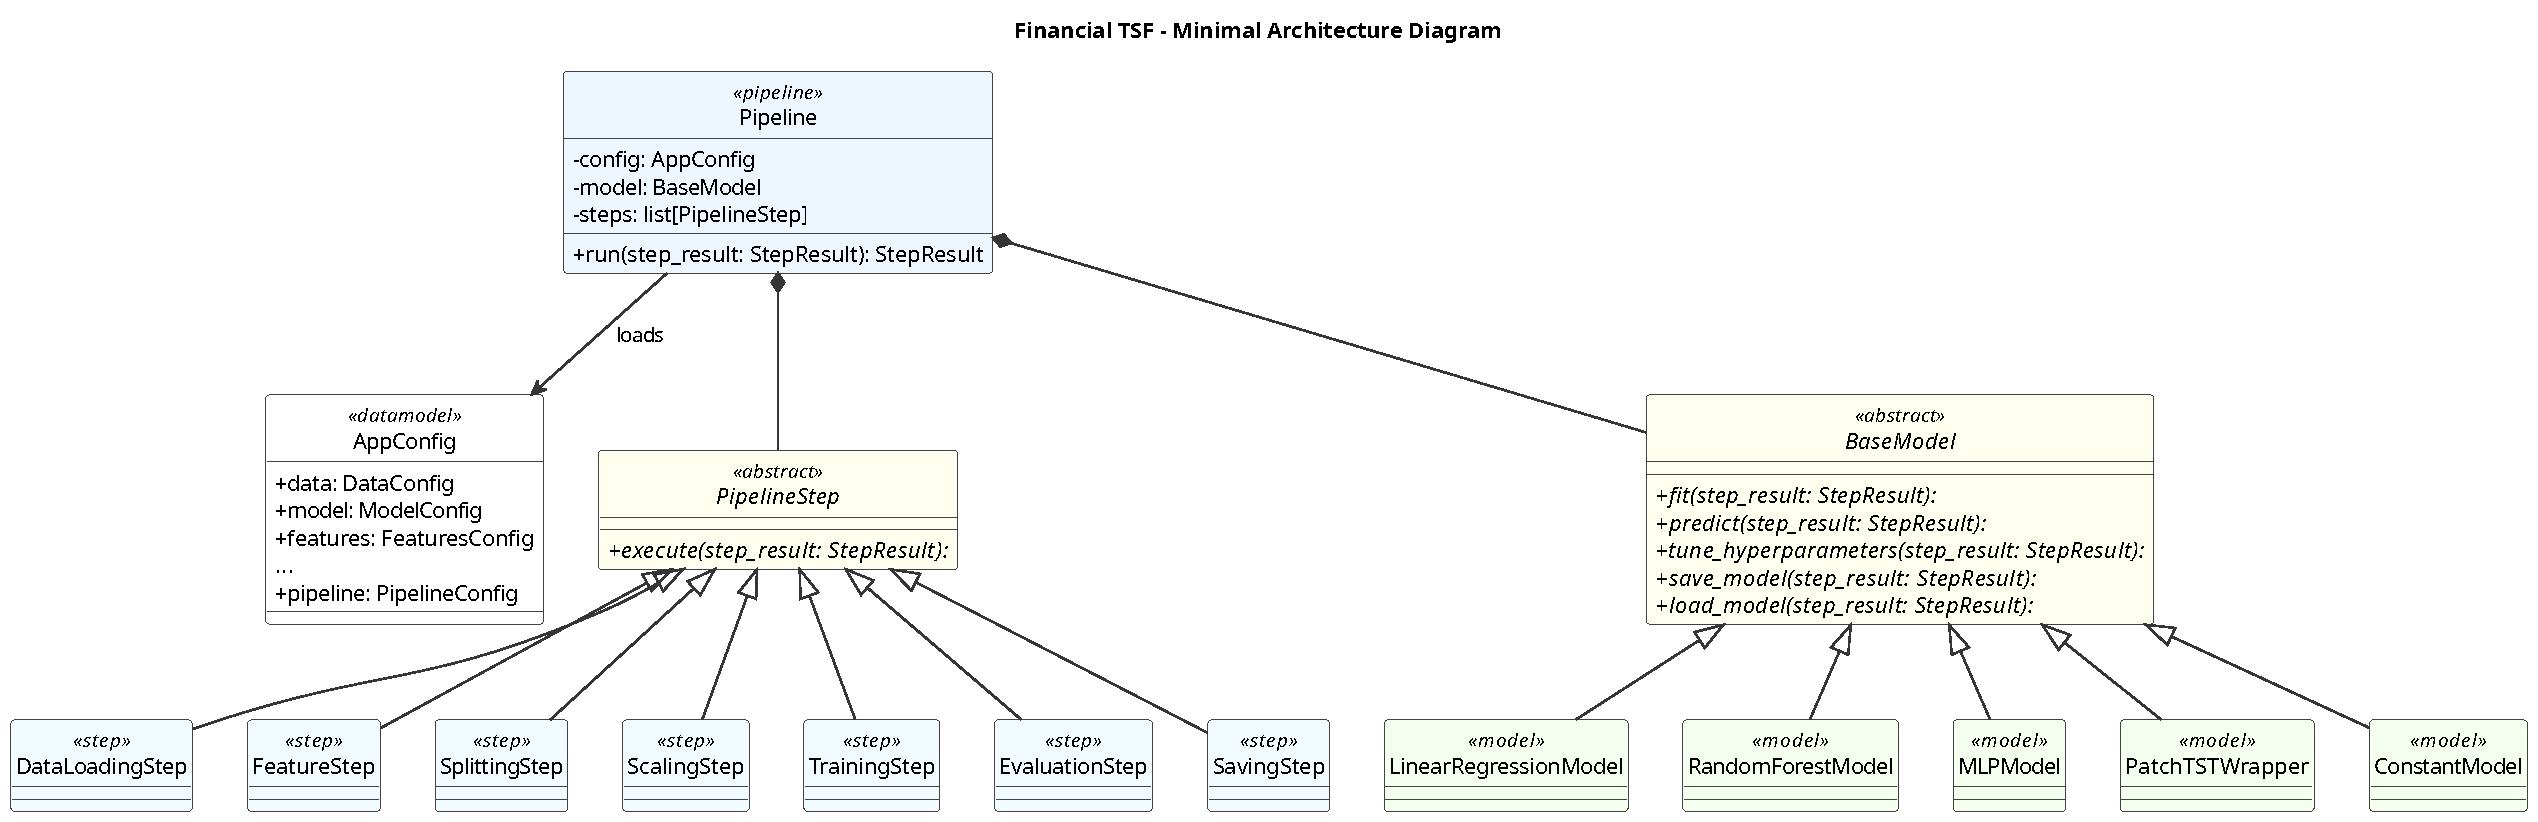
\includegraphics[width=1\linewidth]{plots/architecture/FinancialTSF_Minimal_Architecture.pdf}
    \caption[High-level architecture of the code repository]{High-level architecture of the code repository, highlighting the abstract base classes and their concrete implementations.}
    \label{fig:architecture_setup}
\end{figure}


\section{Pipeline Execution Workflow}

The pipeline iterates through the defined steps sequentially. Each step performs a specific task, storing the results in the \texttt{StepResult} object for the next step:

\paragraph{\texttt{DataLoadingStep}:}
This step loads all CSV files containing the \gls{ohlcv} data based on the configuration. Data validation is performed on each ticker individually to ensure consistency across the selected date range.

\paragraph{\texttt{FeatureStep}:}
This step computes the technical indicators defined in the \texttt{featureconfig.json} (Appendix \ref{app:feature_config_json}). This configuration also acts as the mapping of features to their respective complexity levels. Only features corresponding to the active complexity levels from the file are calculated. 

\paragraph{\texttt{SplittingStep}:}
This step determines the global splitting timestamps based on the ticker with the largest available date range (for training, validation and testing datasets).

\paragraph{\texttt{NormalizingStep}:}
This step implements a two-stage preprocessing setup. First \textbf{Winsorization} (clipping) is applied to the features based on the training set distribution. Second, a \texttt{RobustScaler} is fitted on the training data exclusively and applied to the validation and test sets to prevent data leakage. 

\paragraph{\texttt{TrainingStep}:}
This step manages the models training and fitting process. If enabled, hyperparameter optimization is performed to identify the best configuration using the validation set. 
Next, the model is fitted on the training data either with a default set of hyperparameters or using the best-performing set from the previous optimization run. Using the fitted model, all specified horizons are predicted on the test set. Since all models inherit from a common base interface, the execution logic remains uniform across all architectures (see Appendix \ref{code:class_BaseModel}). 

\paragraph{\texttt{EvaluationStep}:}
This step reverses the scaling of respective data using per-ticker metadata and maps the global prediction dataset back to specific tickers. It computes multi-step performance metrics for both statistical evaluation and economic analysis.

\paragraph{\texttt{SavingStep}:}
This step saves all experimental components including configurations, trained models, metrics and raw predictions into a folder created specifically for the execution. A summary text file concludes the most important aspects of the run stating the corresponding feature list, sample counts, splitting points, training durations and the individual metrics. 





\chapter{Experiments}
\label{ch:experiments}



\section{Data Analysis}
\subsection{Data Selection} 
% Dificult to get free historical data over those interval. from which index companies and sectors. index/ site/ what date is about \gls{ohlcv} - volume(number of tickers) 5min interval...
% how many datapoints... 
The Nasdaq-100 Index was chosen as the data source. The composition of the index was retrieved from the Nasdaq website (\url{https://www.nasdaq.com/market-activity/quotes/nasdaq-ndx-index}, accessed on January 2, 2026).
The observation period ranges from 2015-01-01 to 2023-12-31 with a 5-minute trading interval during regular trading hours (9:30 a.m. to 4:00 p.m.), Monday through Friday.
Historical data was fetched from \texttt{AlphaVantage} for all 101 Tickers. The historical data is only very limited available with a free membership. For reproducibility an own api key is required. The available data for each ticker is \gls{ohlcv} data, consisting of Open, High, Low and Close prices as well as volume (number of traded shares) for each 5-minute interval. Tickers with limited data availability during the specified time interval, due to different \glspl{ipo}, are used starting from their first available trading date. 

% \subsection{Datacleaning} ->why some data is missing of some timestamps? how split point was decided, what to do for companies that didnt where on exchange prior to this date.
% Data is firstly validated with simple sanity checks. 
% if any of the specificied columns is null/ empty
% if high is really the maximum value out of the other columns
% if low is really the minimum value out of the other columns


\subsection{Statistical Analysis}
In financial data, certain domain-specific statistical properties must be adressed before approaching further analysis. A primary issue with raw ticker prices is that they are non-stationary, meaning statistical properties like the mean and variance change over time. This is illustrated in Figure \ref{fig:close_price}. 
% To proof that the data is (non) stataionary statistical tests can be made, in this case the \gls{adf} Test is used. This results in a p-value of 0.9?? for selected AAPL-Ticker. This non stationarity arises with issue as further mentioned. 
Specifically neural networks which were trained on non stationary data will not learn generalizable patterns but specific trends of the training period.
\begin{figure}[htbp]
    \centering
    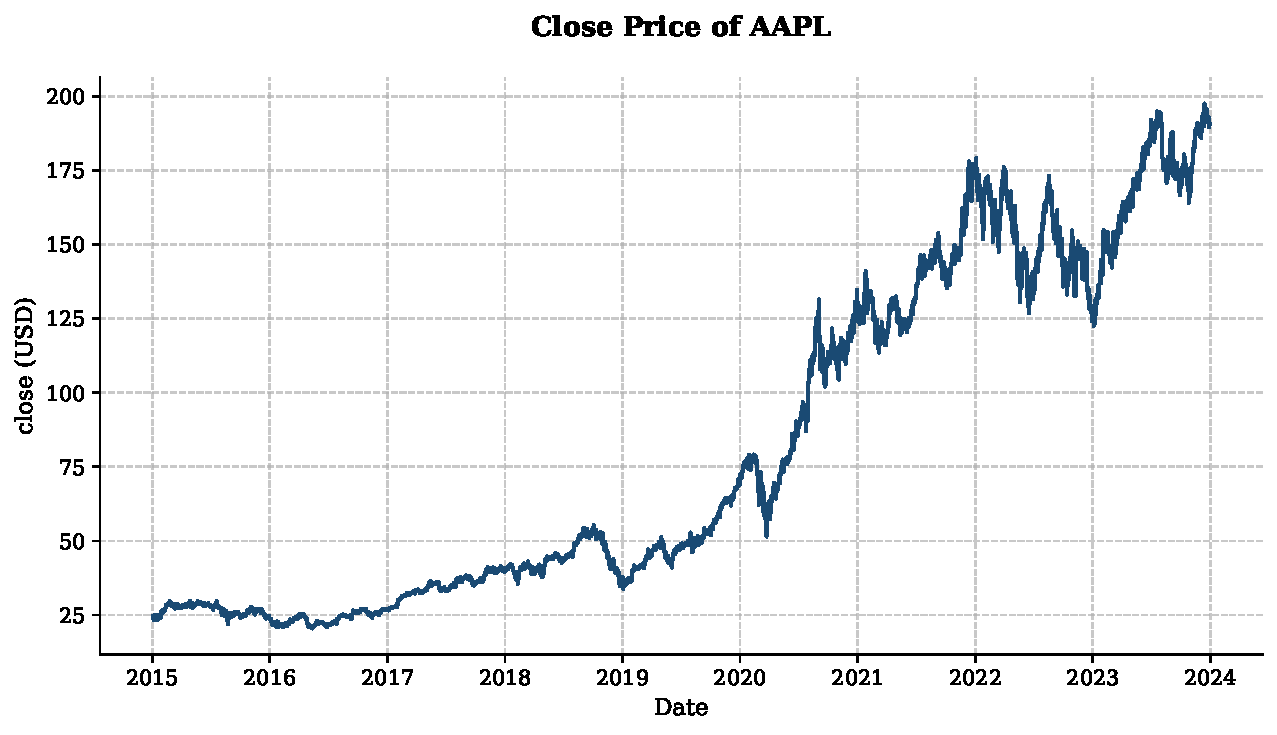
\includegraphics[width=1\linewidth]{plots/eda/close_timeseries.pdf}
    \caption{The Close price in USD of AAPL over 5-minute intervals during the selected observation period}    
    \label{fig:close_price}
\end{figure}

% To remove stationarity differencing and logarithm is used. Using the logarithm in this case also comes with the benefit that 
% \begin{itemize}
%     \item log returns are additive over time - which percentage returns are not. Example calculation
%     \item log returns are symmetric an increase of 0.5 will be the same as an decrease of 0.5 -> define better
%     Result: Extreme outliers happen to be more often in the 5min interval than following a normal distribution. (why use of robust scaler/ Mamba/transformer
%     \end{itemize}

After applying the log-return the following plot can be examined (Figure \ref{fig:logret_timeseries}). The log-returns follow a relative stationary nature.

Another property of financial returns is that  their distribution typically follow a distribution with fat tails and high kurtosis compared to a normal distribution (Figure \ref{fig:logret_dist}). 

\begin{figure}[htbp]
    \centering
    \begin{subfigure}[b]{0.49\textwidth}
        \centering
        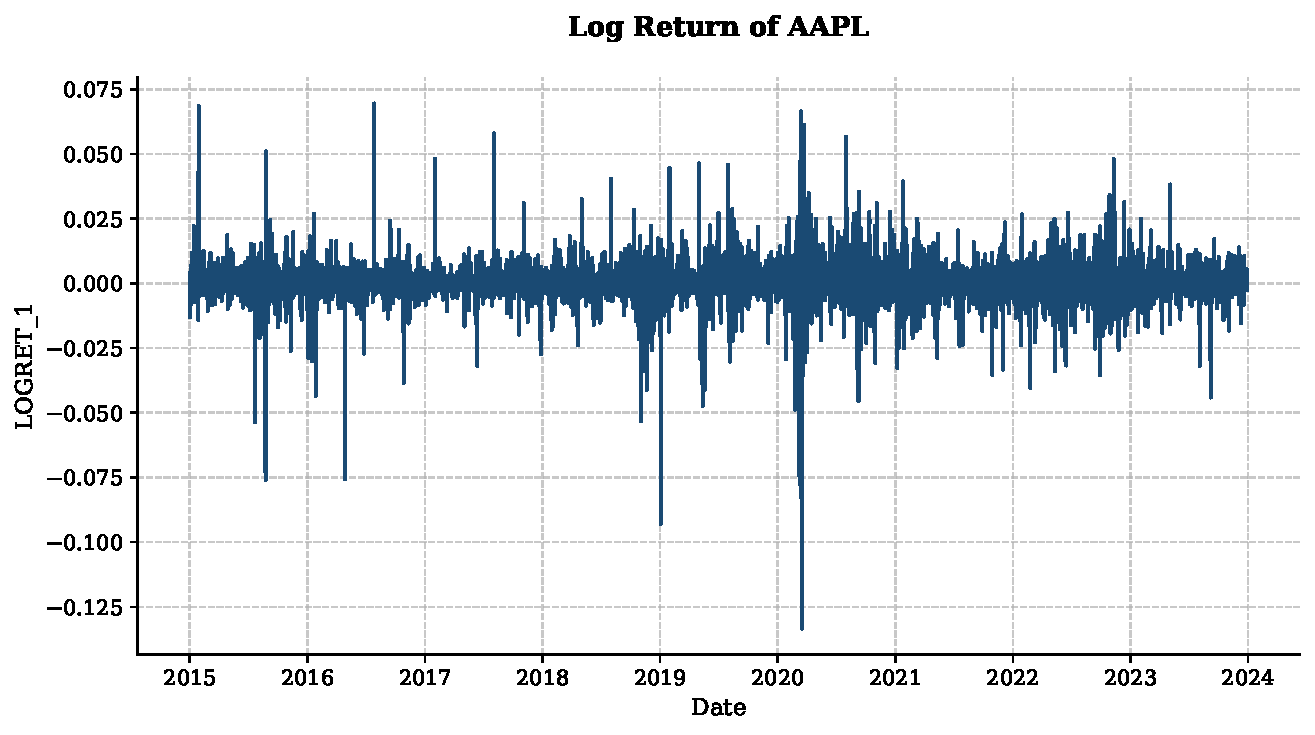
\includegraphics[width=\textwidth]{plots/eda/LOGRET_1_timeseries.pdf}
        \caption{Time series of returns.}
        \label{fig:logret_timeseries}
    \end{subfigure}
    \hfill 
    \begin{subfigure}[b]{0.49\textwidth}
        \centering
        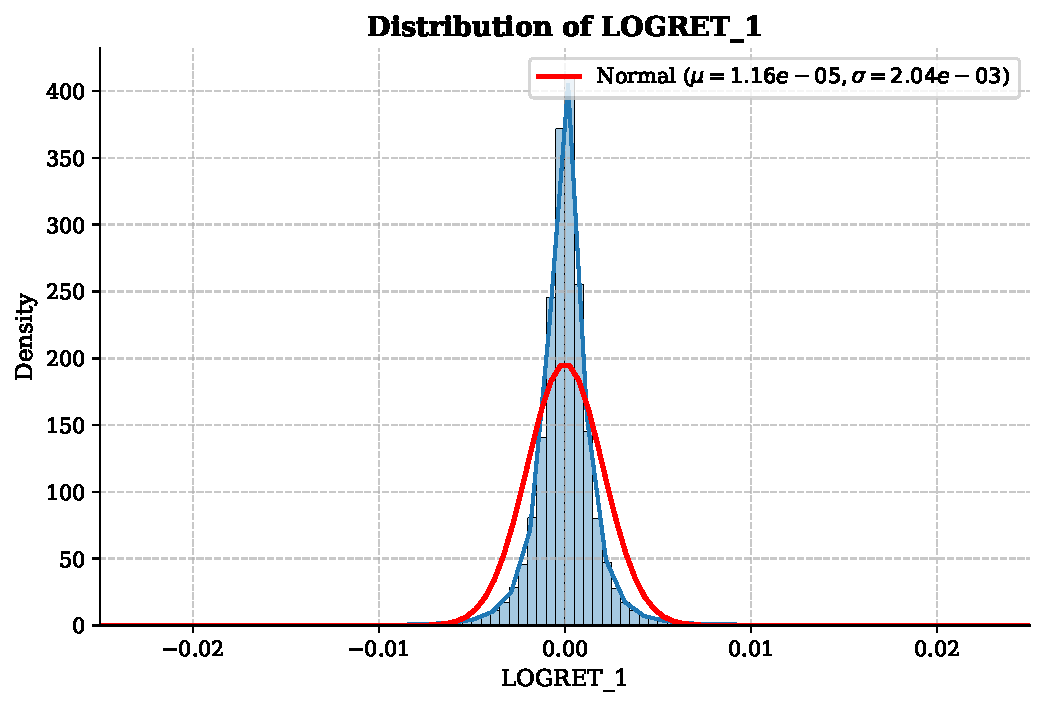
\includegraphics[width=\textwidth]{plots/eda/LOGRET_1_dist.pdf}
        \caption{Distribution analysis.}
        \label{fig:logret_dist}
    \end{subfigure}

    \caption[AAPL Log-return Analysis]{Analysis of 5-minute log-returns for AAPL. \textbf{Left:}  The plot illustrates the stationarity of the returns and the presence of volatility clustering throughout the dataset period. The log-return fluctuates around 0, although some big outliers can be observed. \textbf{Right:} Distribution of 5-minute log-returns for LOGRET\_1 (The log-return of previous 5-min interval). The plot compares the log-return distribution against a theoretical normal distribution with corresponding $\mu$ and $\sigma$ of the distribution.}
    \label{fig:combined_logret}
\end{figure}


Analyzing the volume reveals significant deviations from a normal distribution. As illustrated in the raw volume distribution (see Figure \ref{fig:vol_dist}), the data reveals a strong positive skewness. The high variance relative to the mean highlights the presence of extreme outliers. These outliers are primarily caused by the intraday dynamics of the stock market. As shown in the intraday volume graph (Figure \ref{fig:volume_daily}), the volume represents a U-shaped pattern. Significant spikes during the market opening at 09:30 a.m. and the market close at 4:00 p.m. can be observed. To reduce the impact of outliers, a log-transformation was applied. This transforms the distribution into a more bell-shaped curve (see Figure \ref{fig:log_vol_dist})

The analysis for returns was performed only on the close price of the 5-minute interval. The open, high, low, and close prices are highly correlated, especially in short intervals like 5-minutes and would result in nearly the exact same statistical properties and distributions.

\begin{figure}[htbp]
    \centering
    \begin{subfigure}[b]{0.49\textwidth}
        \centering
        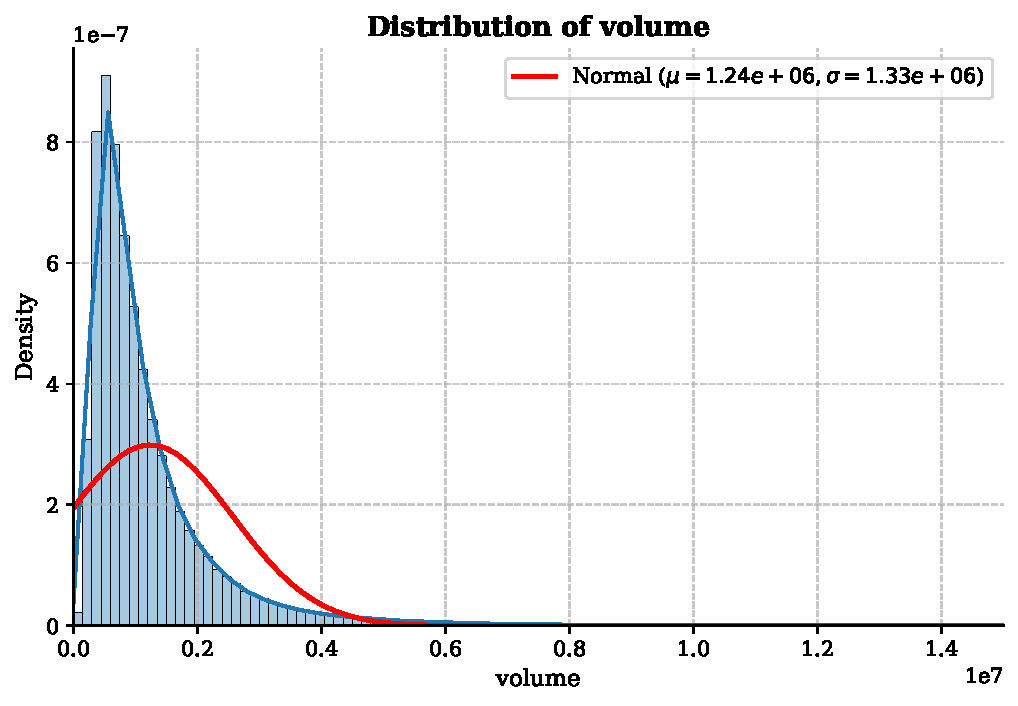
\includegraphics[width=\textwidth]{plots/eda/volume_dist.pdf}
        \caption{Distribution of volume.}
        \label{fig:vol_dist}
    \end{subfigure}
    \hfill
    \begin{subfigure}[b]{0.49\textwidth}
        \centering
        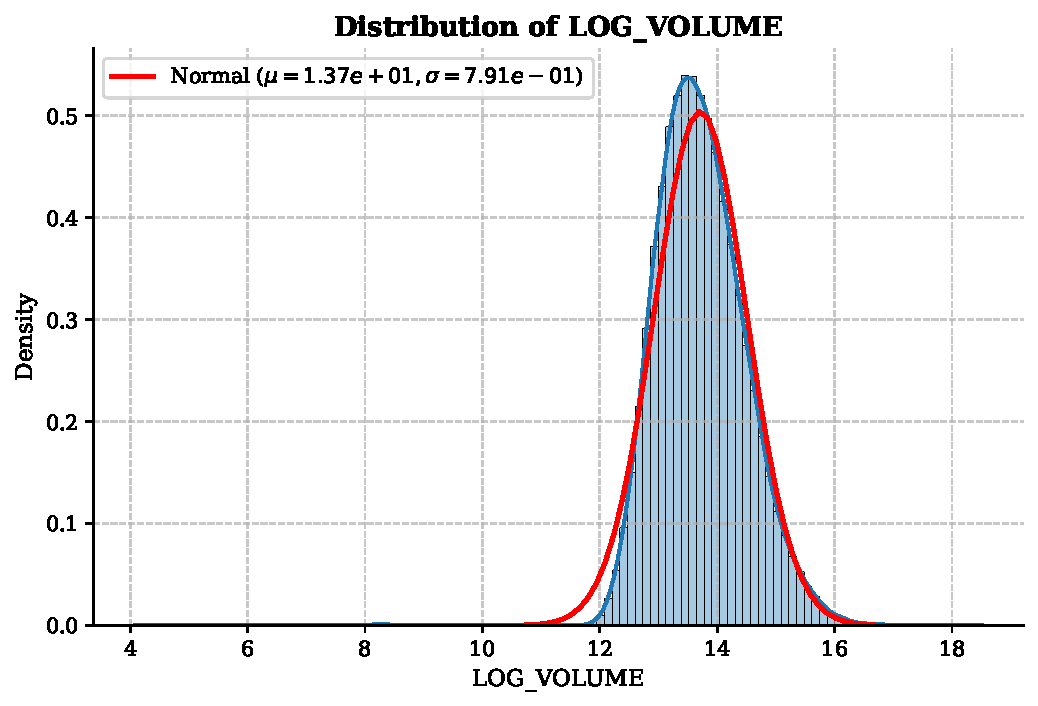
\includegraphics[width=\textwidth]{plots/eda/LOG_VOLUME_dist.pdf}
        \caption{Distribution of log-volume.}
        \label{fig:log_vol_dist}
    \end{subfigure}

    \caption[AAPL Log Volume Analysis]{Analysis of 5-minute log-volume for AAPL. \textbf{Left:} The time series shows log-volume where slight distribution shifts can be observed. \textbf{Right:} The distribution of log-transformed volume compared to a normal distribution with the properties of the underlying dataset ($\mu, \sigma$). }
    \label{fig:combined_log_volume}
\end{figure}

\begin{figure}[htbp]
    \centering
    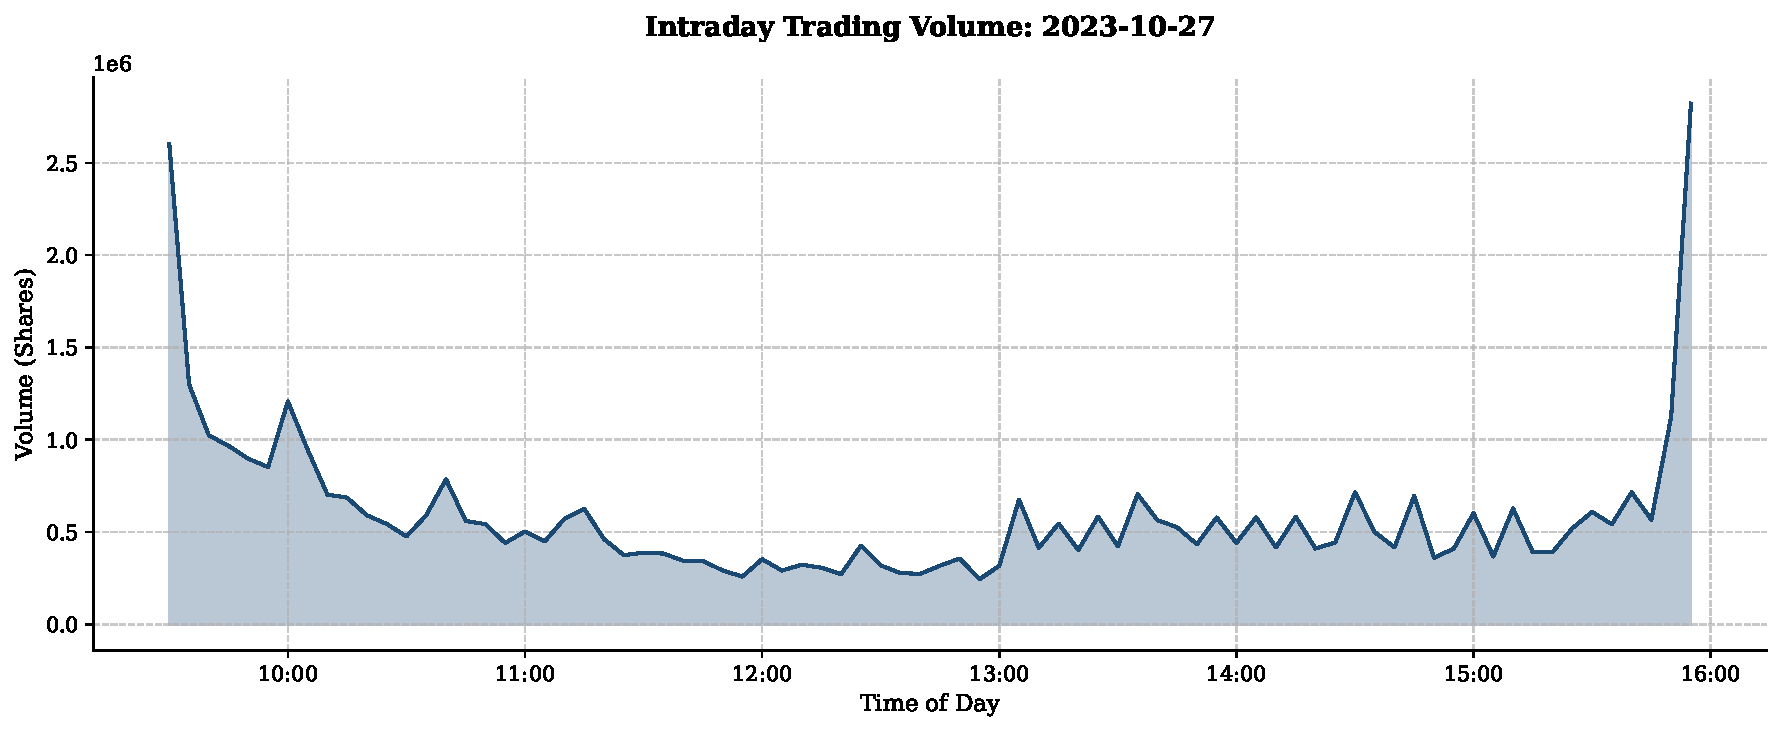
\includegraphics[width=1\linewidth]{plots/eda/volume_2023-10-27.pdf}
    \caption{AAPL volume for a randomly selected day (2023-10-27). Volume spikes at the opening and closing times of the stock exchange can be observed.}
    \label{fig:volume_daily}
\end{figure}

\subsection{Data Partitioning}
Following the feature engineering and target generation process, the dataset consists of complete feature-target pairs for each timestamp across all tickers. To evaluate the model performance and generalization capability, the data is partitioned into three distinct subsets: training, validation, and testing.
This step is done chronologically to respect the temporal order of financial data, avoiding any look-ahead bias. The partition ratios are defined as follows: 
\begin{itemize} 
    \item \textbf{Training Set (75\%)}: Selected to optimize the model parameters (weights) during learning process. 
    \item \textbf{Validation Set (15\%)}: Used for hyperparameter tuning and to prevent overfitting with early stopping during the training of neural networks. 
    \item \textbf{Testing Set (10\%)} Reserved for the final out-of-sample evaluation. This set is used to calculate model performance metrics and economic evaluation. 
\end{itemize}

Since the dataset comprises multiple tickers with different listing dates, a per-ticker split would result in inconsistent time splits (e.g. the training period for Ticker 1 might overlap with the testing period of Ticker 2). To prevent this, a global time-split strategy was implemented across all tickers. The ticker with the longest historical data serves as the reference to determine the absolute calendar timestamps for the split points.
%  ($T_{val\_start}$ and $T_{test\_start}$).
All tickers are then split based on these global split points. This ensures that the model is never trained on future market regimes of other assets.
With this strategy applied, it is possible for individual tickers to have missing data because they were not listed at that time. Tickers that did not comprise at least two years of available data in the training set were excluded from the study. This exclusion is justified because the model cannot learn the specific patterns of the ticker during training and would therefore generalize poorly in testing. 
\begin{figure}[htbp]
    \centering
    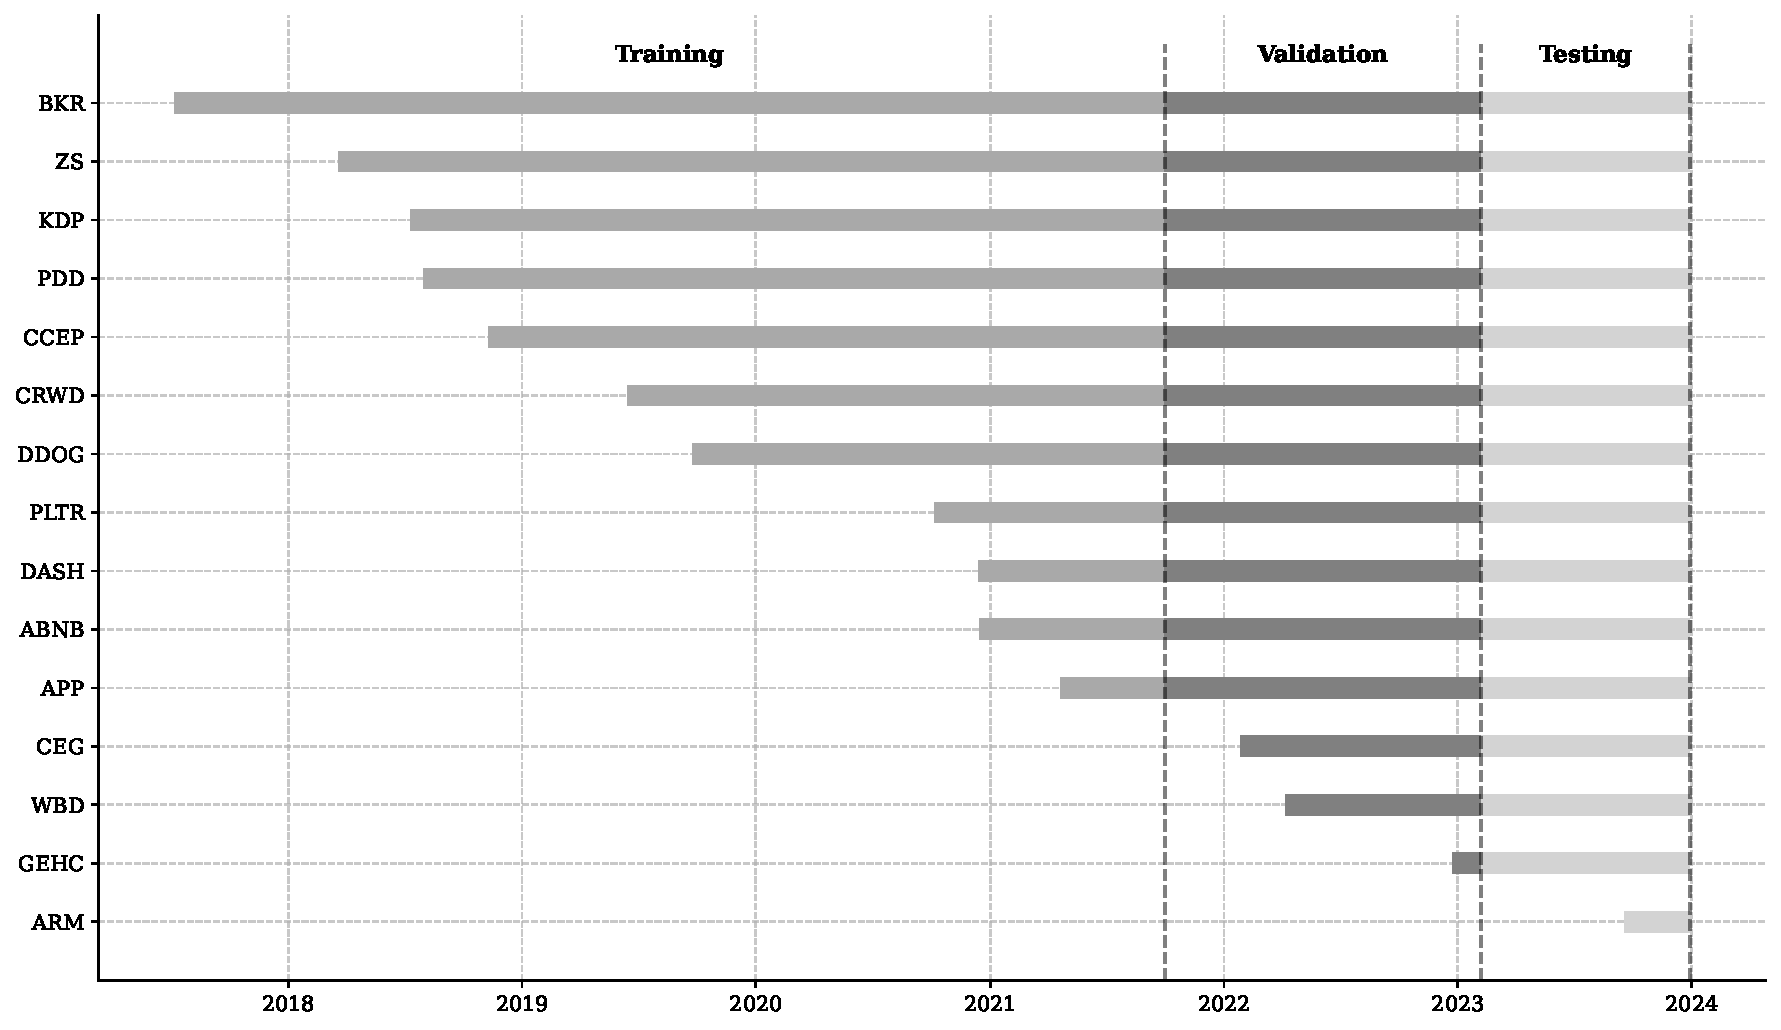
\includegraphics[width=1\linewidth]{plots/eda/splitting_step/splitpoints_alltickers_2015-01-01_2023-12-31.pdf}
    \caption{Data availability of the top 15 tickers sorted by their first available timestamp  in descending order. Start point for the validation set: 2021-09-30. Start point for the  testing set: 2023-02-06.}
    \label{fig:splitpoints}
\end{figure}
Applying this strategy reduced the number of assets from 101 to 92 tickers. Figure \ref{fig:splitpoints} illustrates the data availability and the global split lines.
In this case, out of 101 Tickers, were 9 removed after applying this strategy. 


\subsection{Preprocessing}
\subsubsection{Handling Outliers}
Since log-returns in financial time series follow leptokurtic distributions as previously discussed, a multi-stage preprocessing pipeline is applied. To prevent extreme values from distorting the parameters of the subsequent scaling process, the input features are first winsorized. For each ticker $n$, all feature values below the 1st percentile and above the 99th percentile are capped at these thresholds. This approach aims to reduce the impact of extreme outliers in the dataset while retaining the underlying information. The distribution of three example features is first visualized without any preprocessing (see Figure \ref{fig:boxplot_unscaled}) and then after winsorization has been applied (see Figure \ref{fig:boxplot_winsorized_1.0_percentiles}). This comparison shows the impact of outliers on the data distribution.

\begin{figure}[htbp]
    \centering
    \begin{subfigure}[b]{0.32\textwidth}
        \centering
        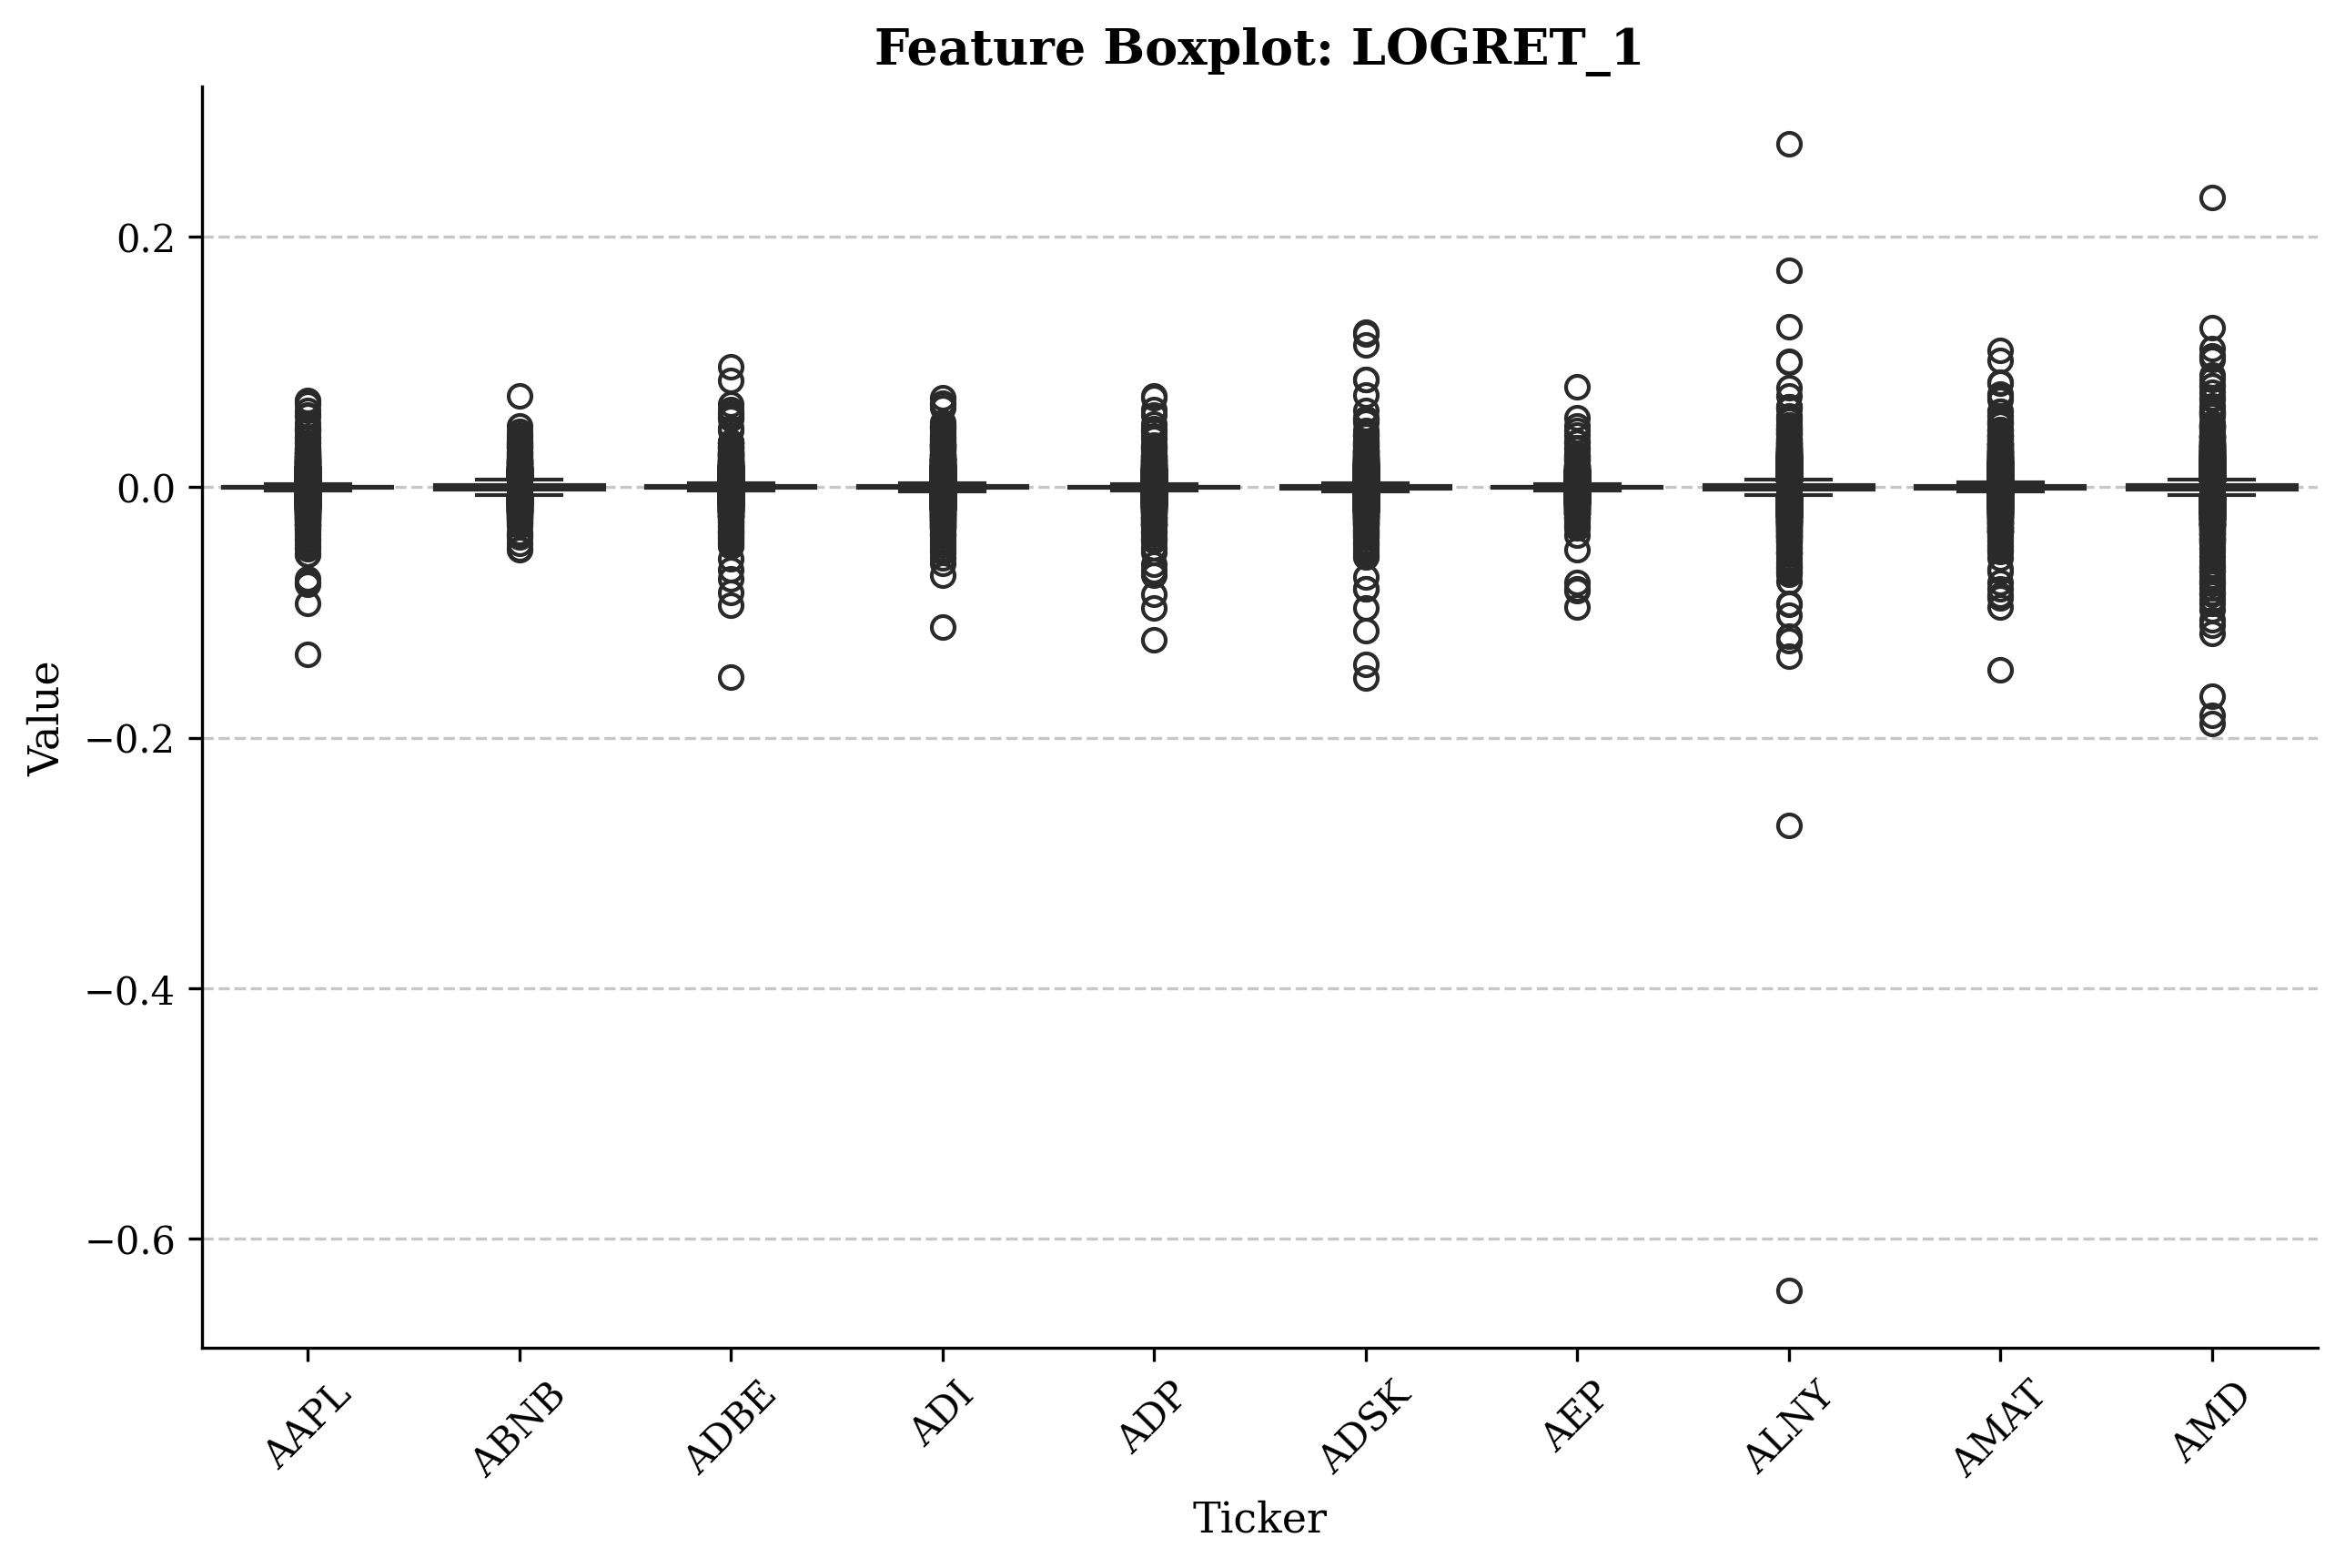
\includegraphics[width=\textwidth]{plots/boxplots/unscaled/LOGRET_1_boxplot.png}
        \caption{Boxplot for log-return.}
        \label{fig:boxplot_unscaled_LOGRET_1}
    \end{subfigure}
    \hfill
    \begin{subfigure}[b]{0.32\textwidth}
        \centering
        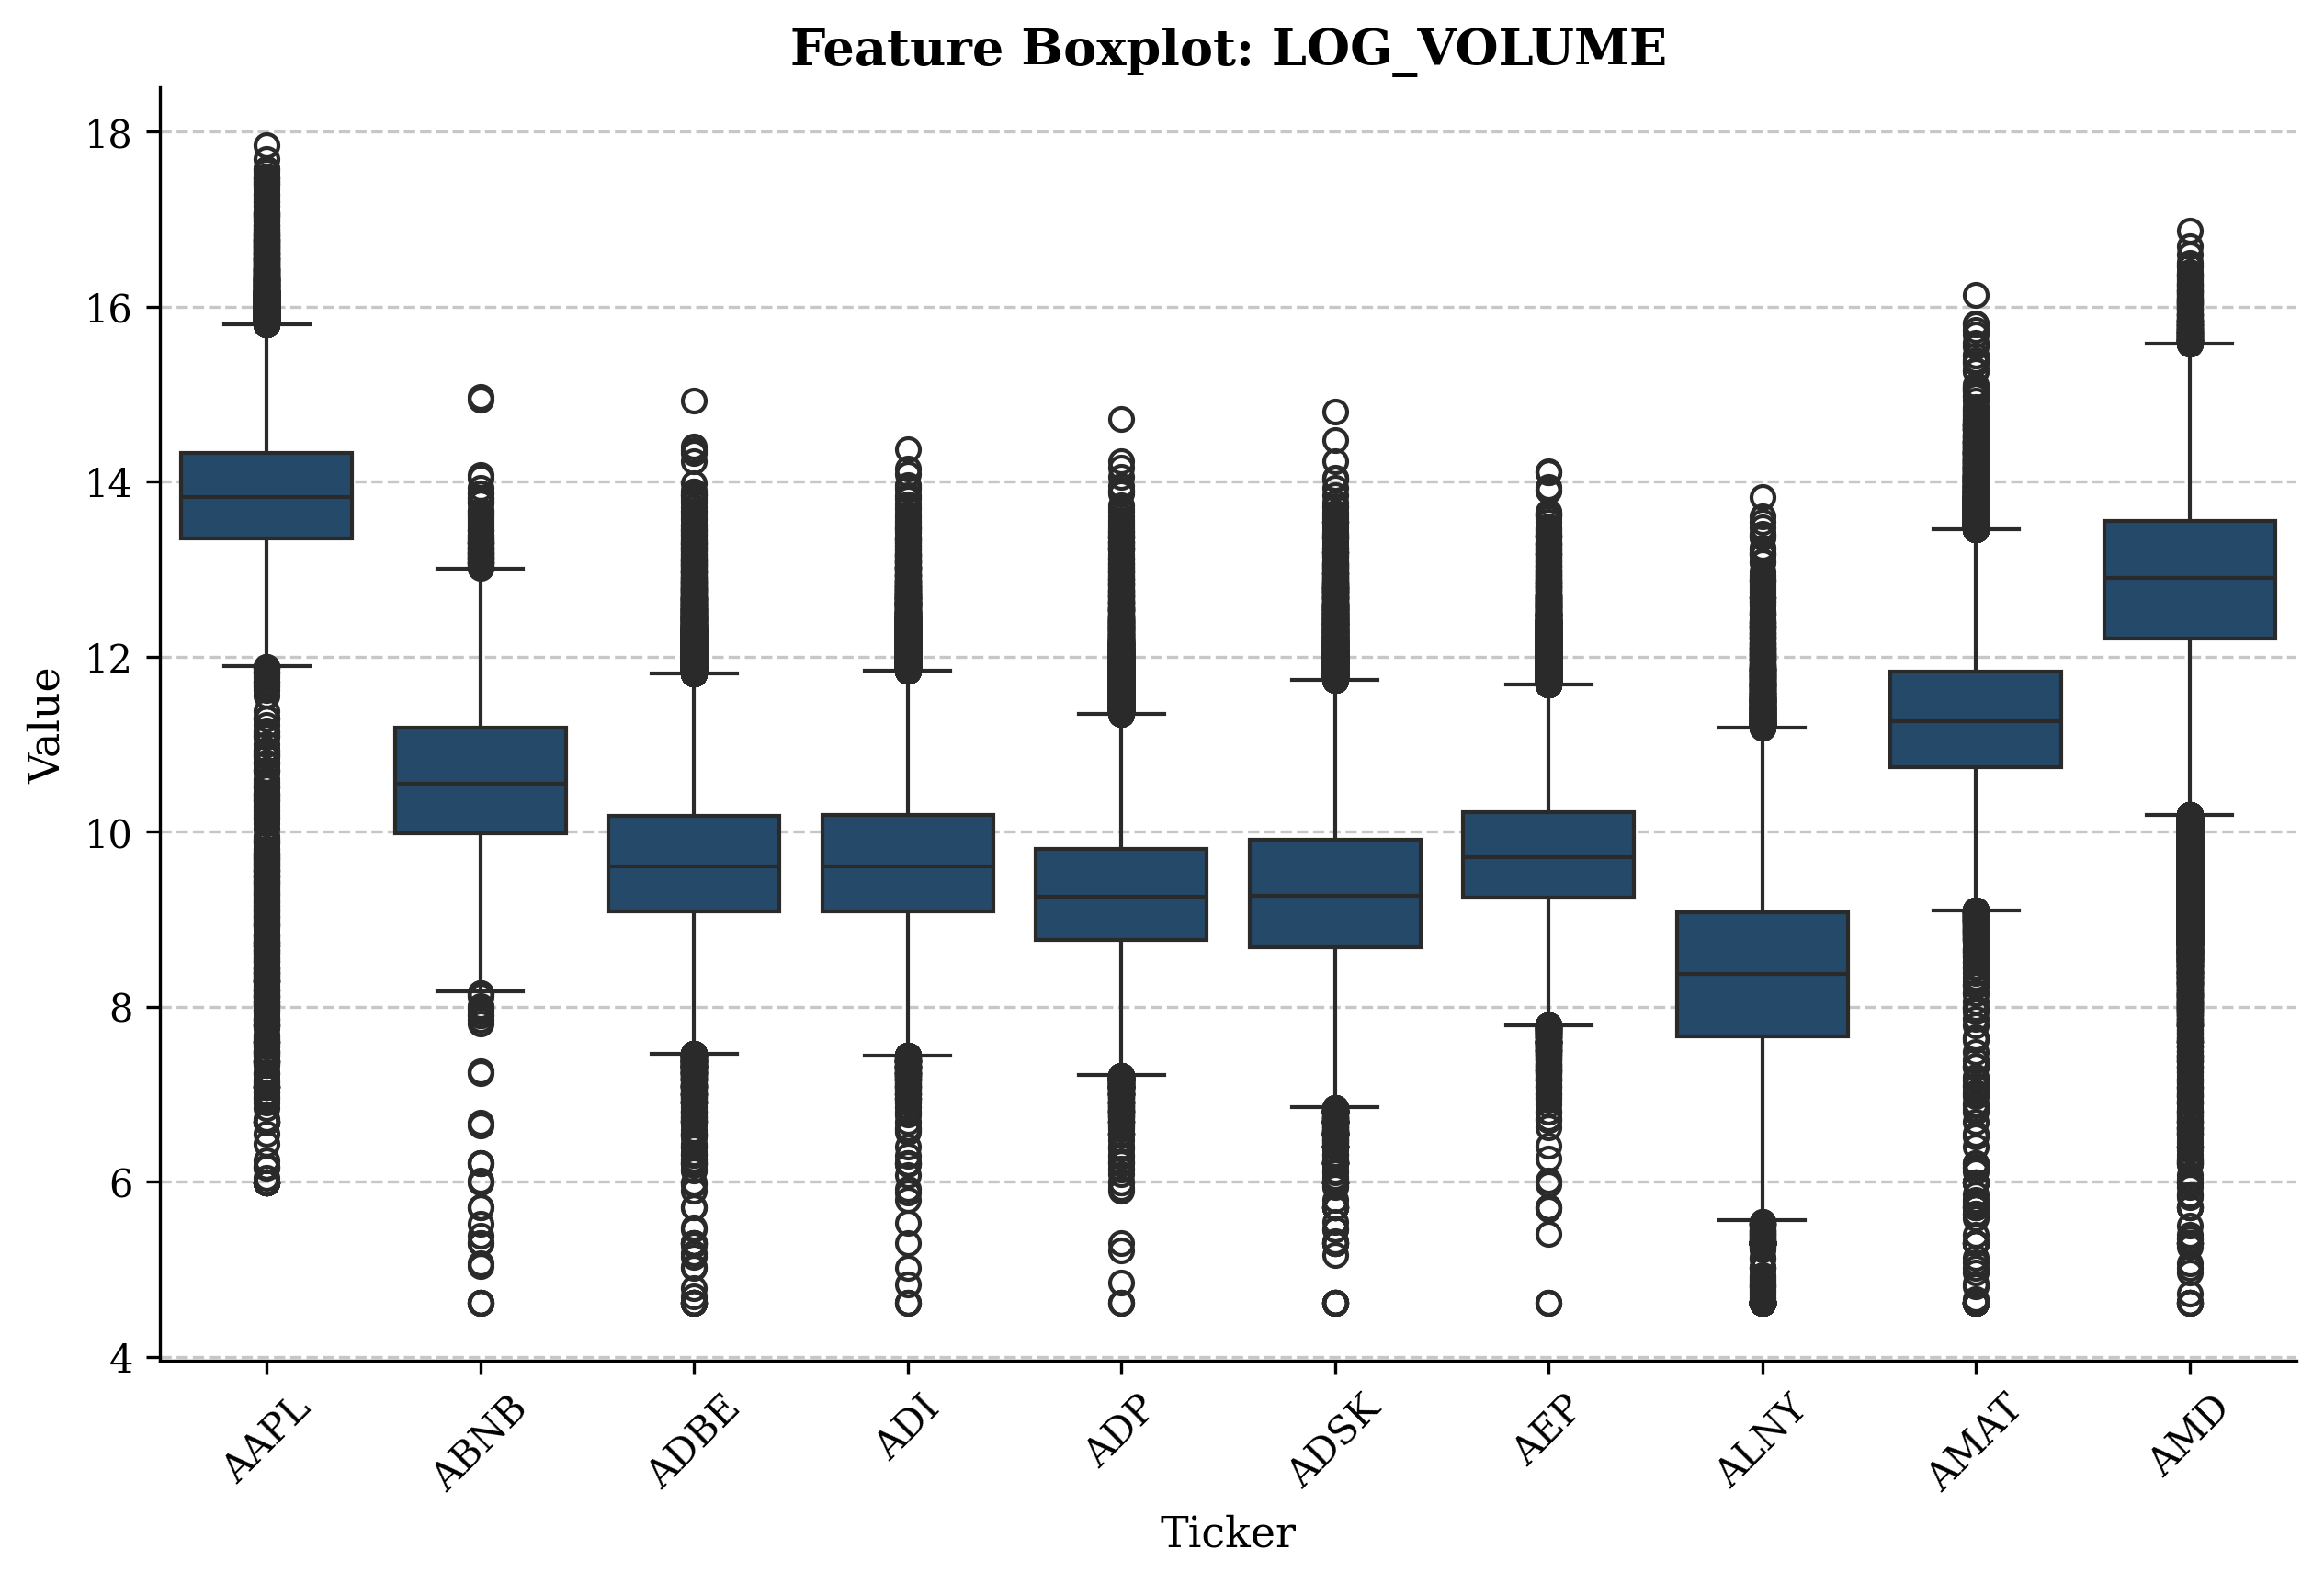
\includegraphics[width=\textwidth]{plots/boxplots/unscaled/LOG_VOLUME_boxplot.png}
        \caption{Boxplot for log-volume.}
        \label{fig:boxplot_unscaled_LOG_VOLUME}
    \end{subfigure}
    \hfill
    \begin{subfigure}[b]{0.32\textwidth}
        \centering
        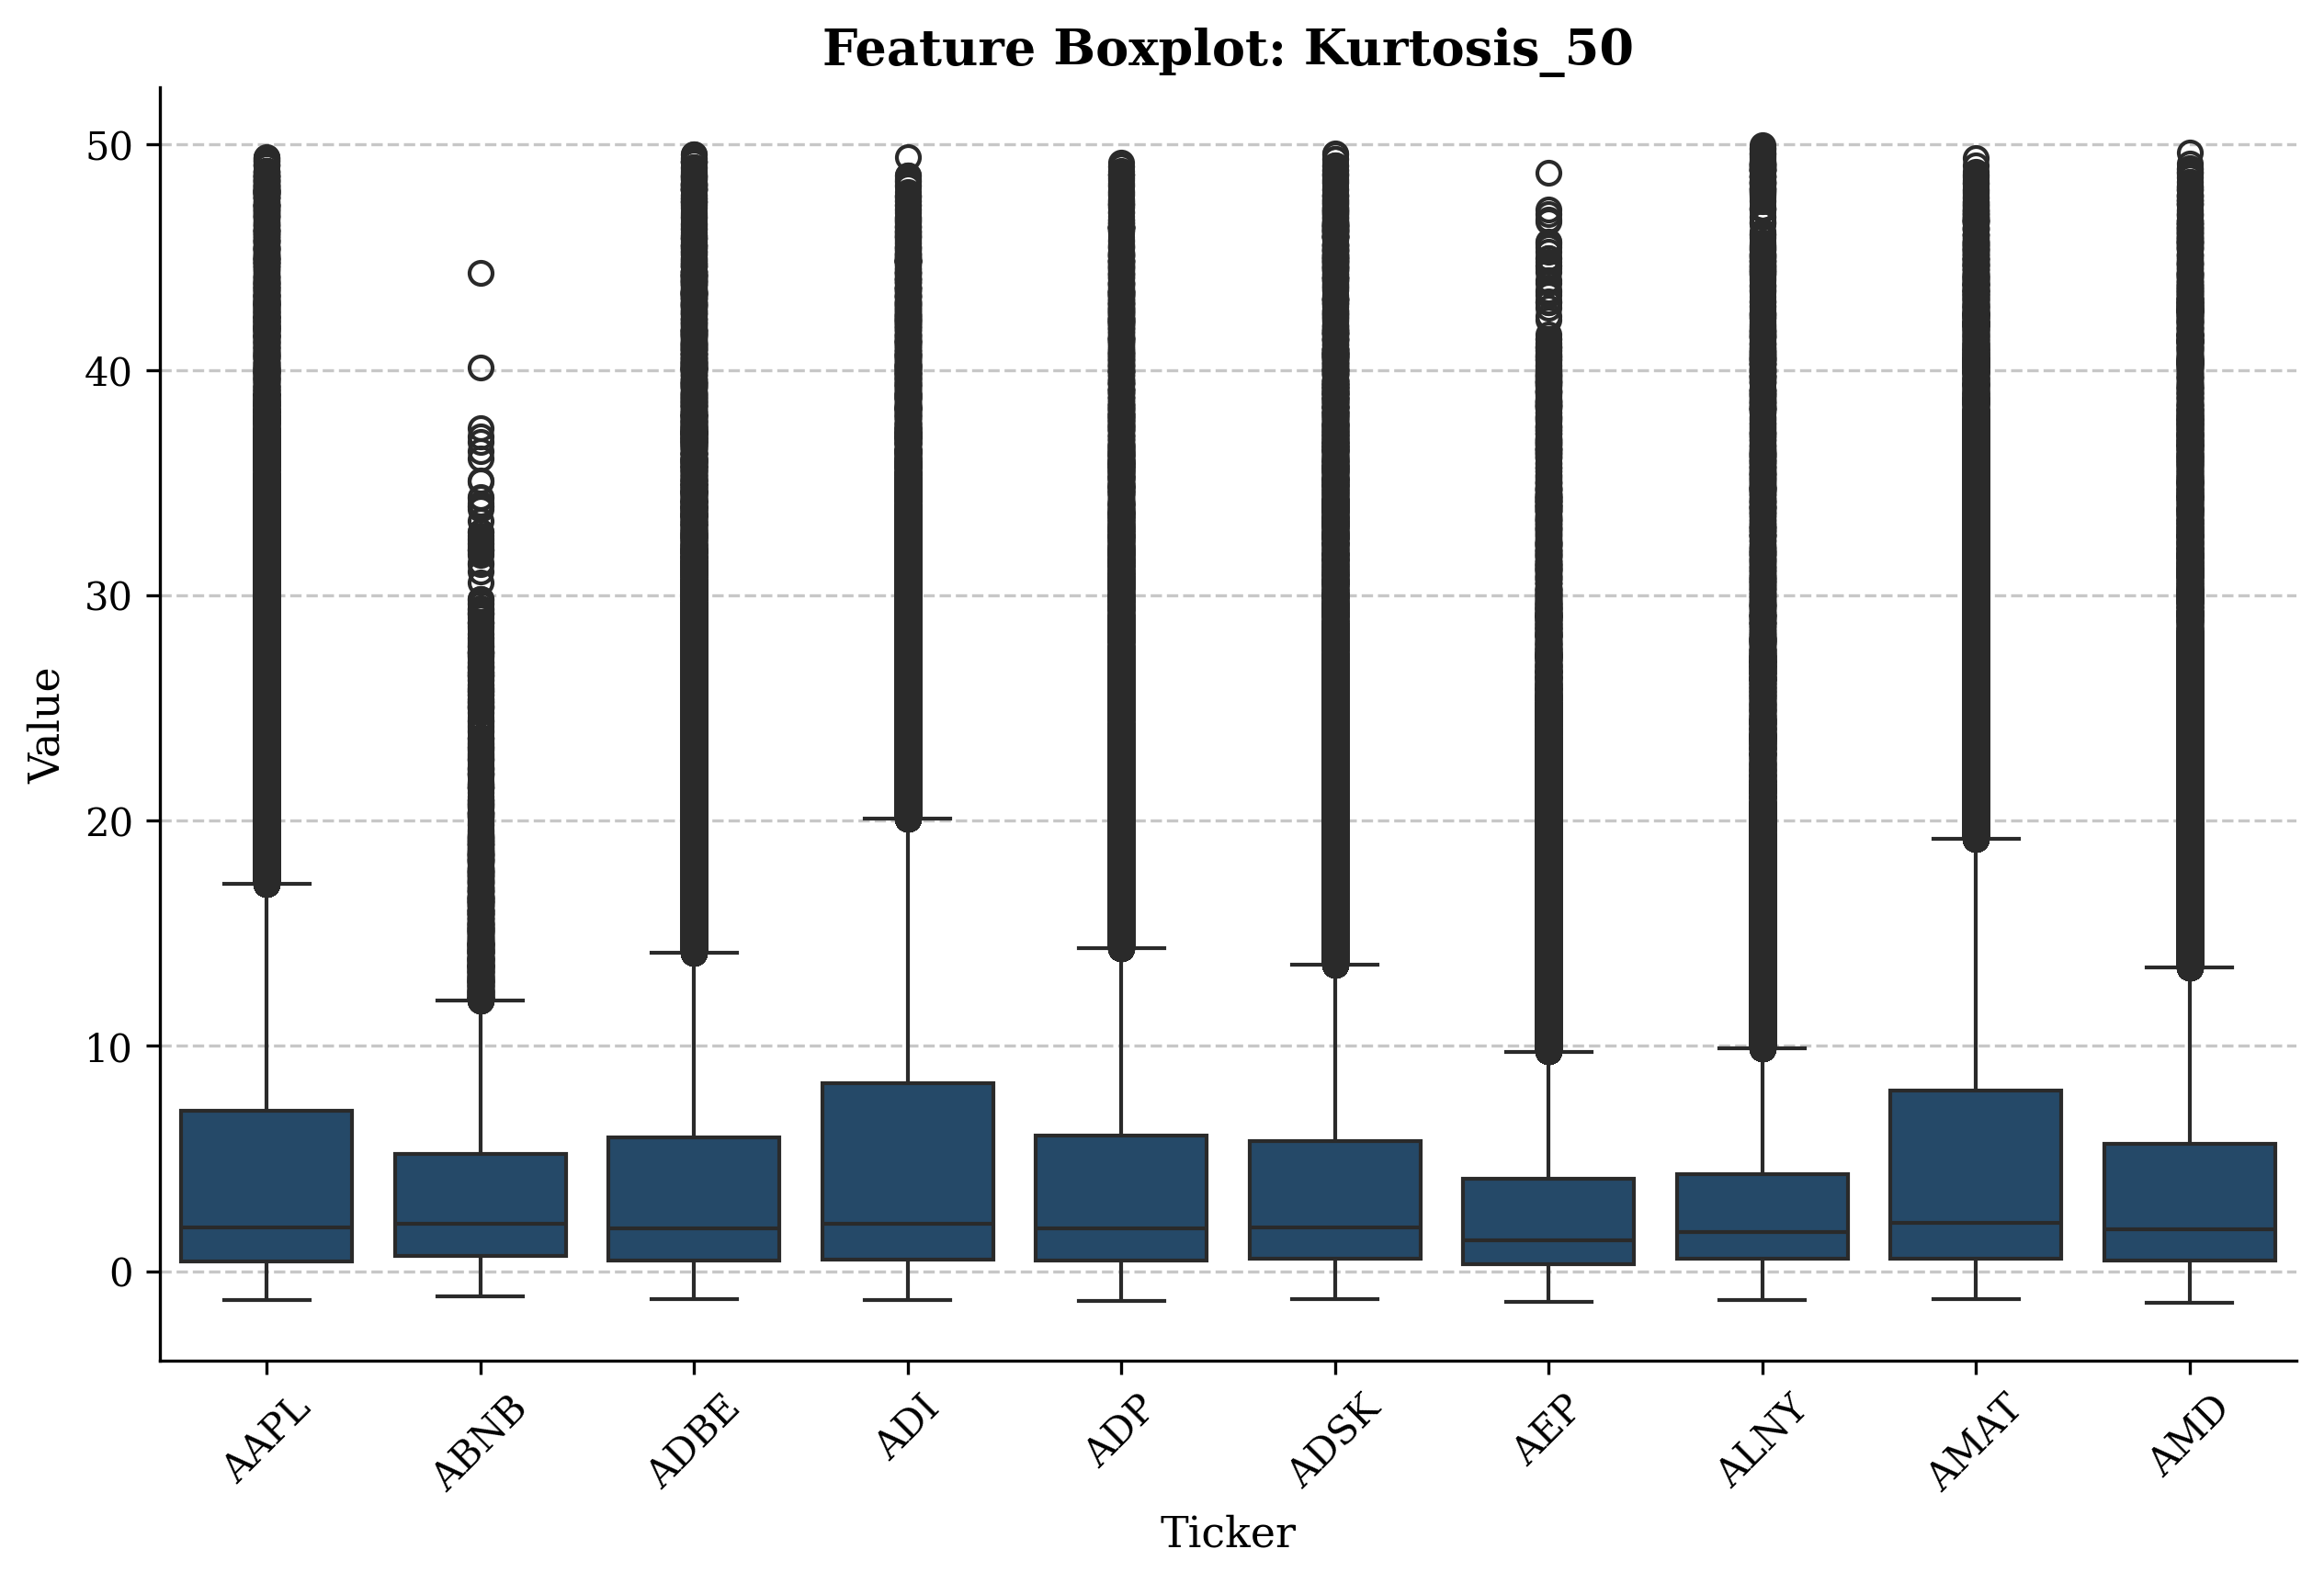
\includegraphics[width=\textwidth]{plots/boxplots/unscaled/Kurtosis_50_boxplot.png}
        \caption{Boxplot for kurtosis.}
        \label{fig:boxplot_unscaled_Kurtosis_50}
    \end{subfigure}

    \caption{Boxplot of unscaled features across 10 selected tickers. It can be observed that the range of the features varies significantly and extreme outliers are present.}
    \label{fig:boxplot_unscaled}
\end{figure}

\begin{figure}[htbp]
    \centering
    \begin{subfigure}[b]{0.32\textwidth}
        \centering
        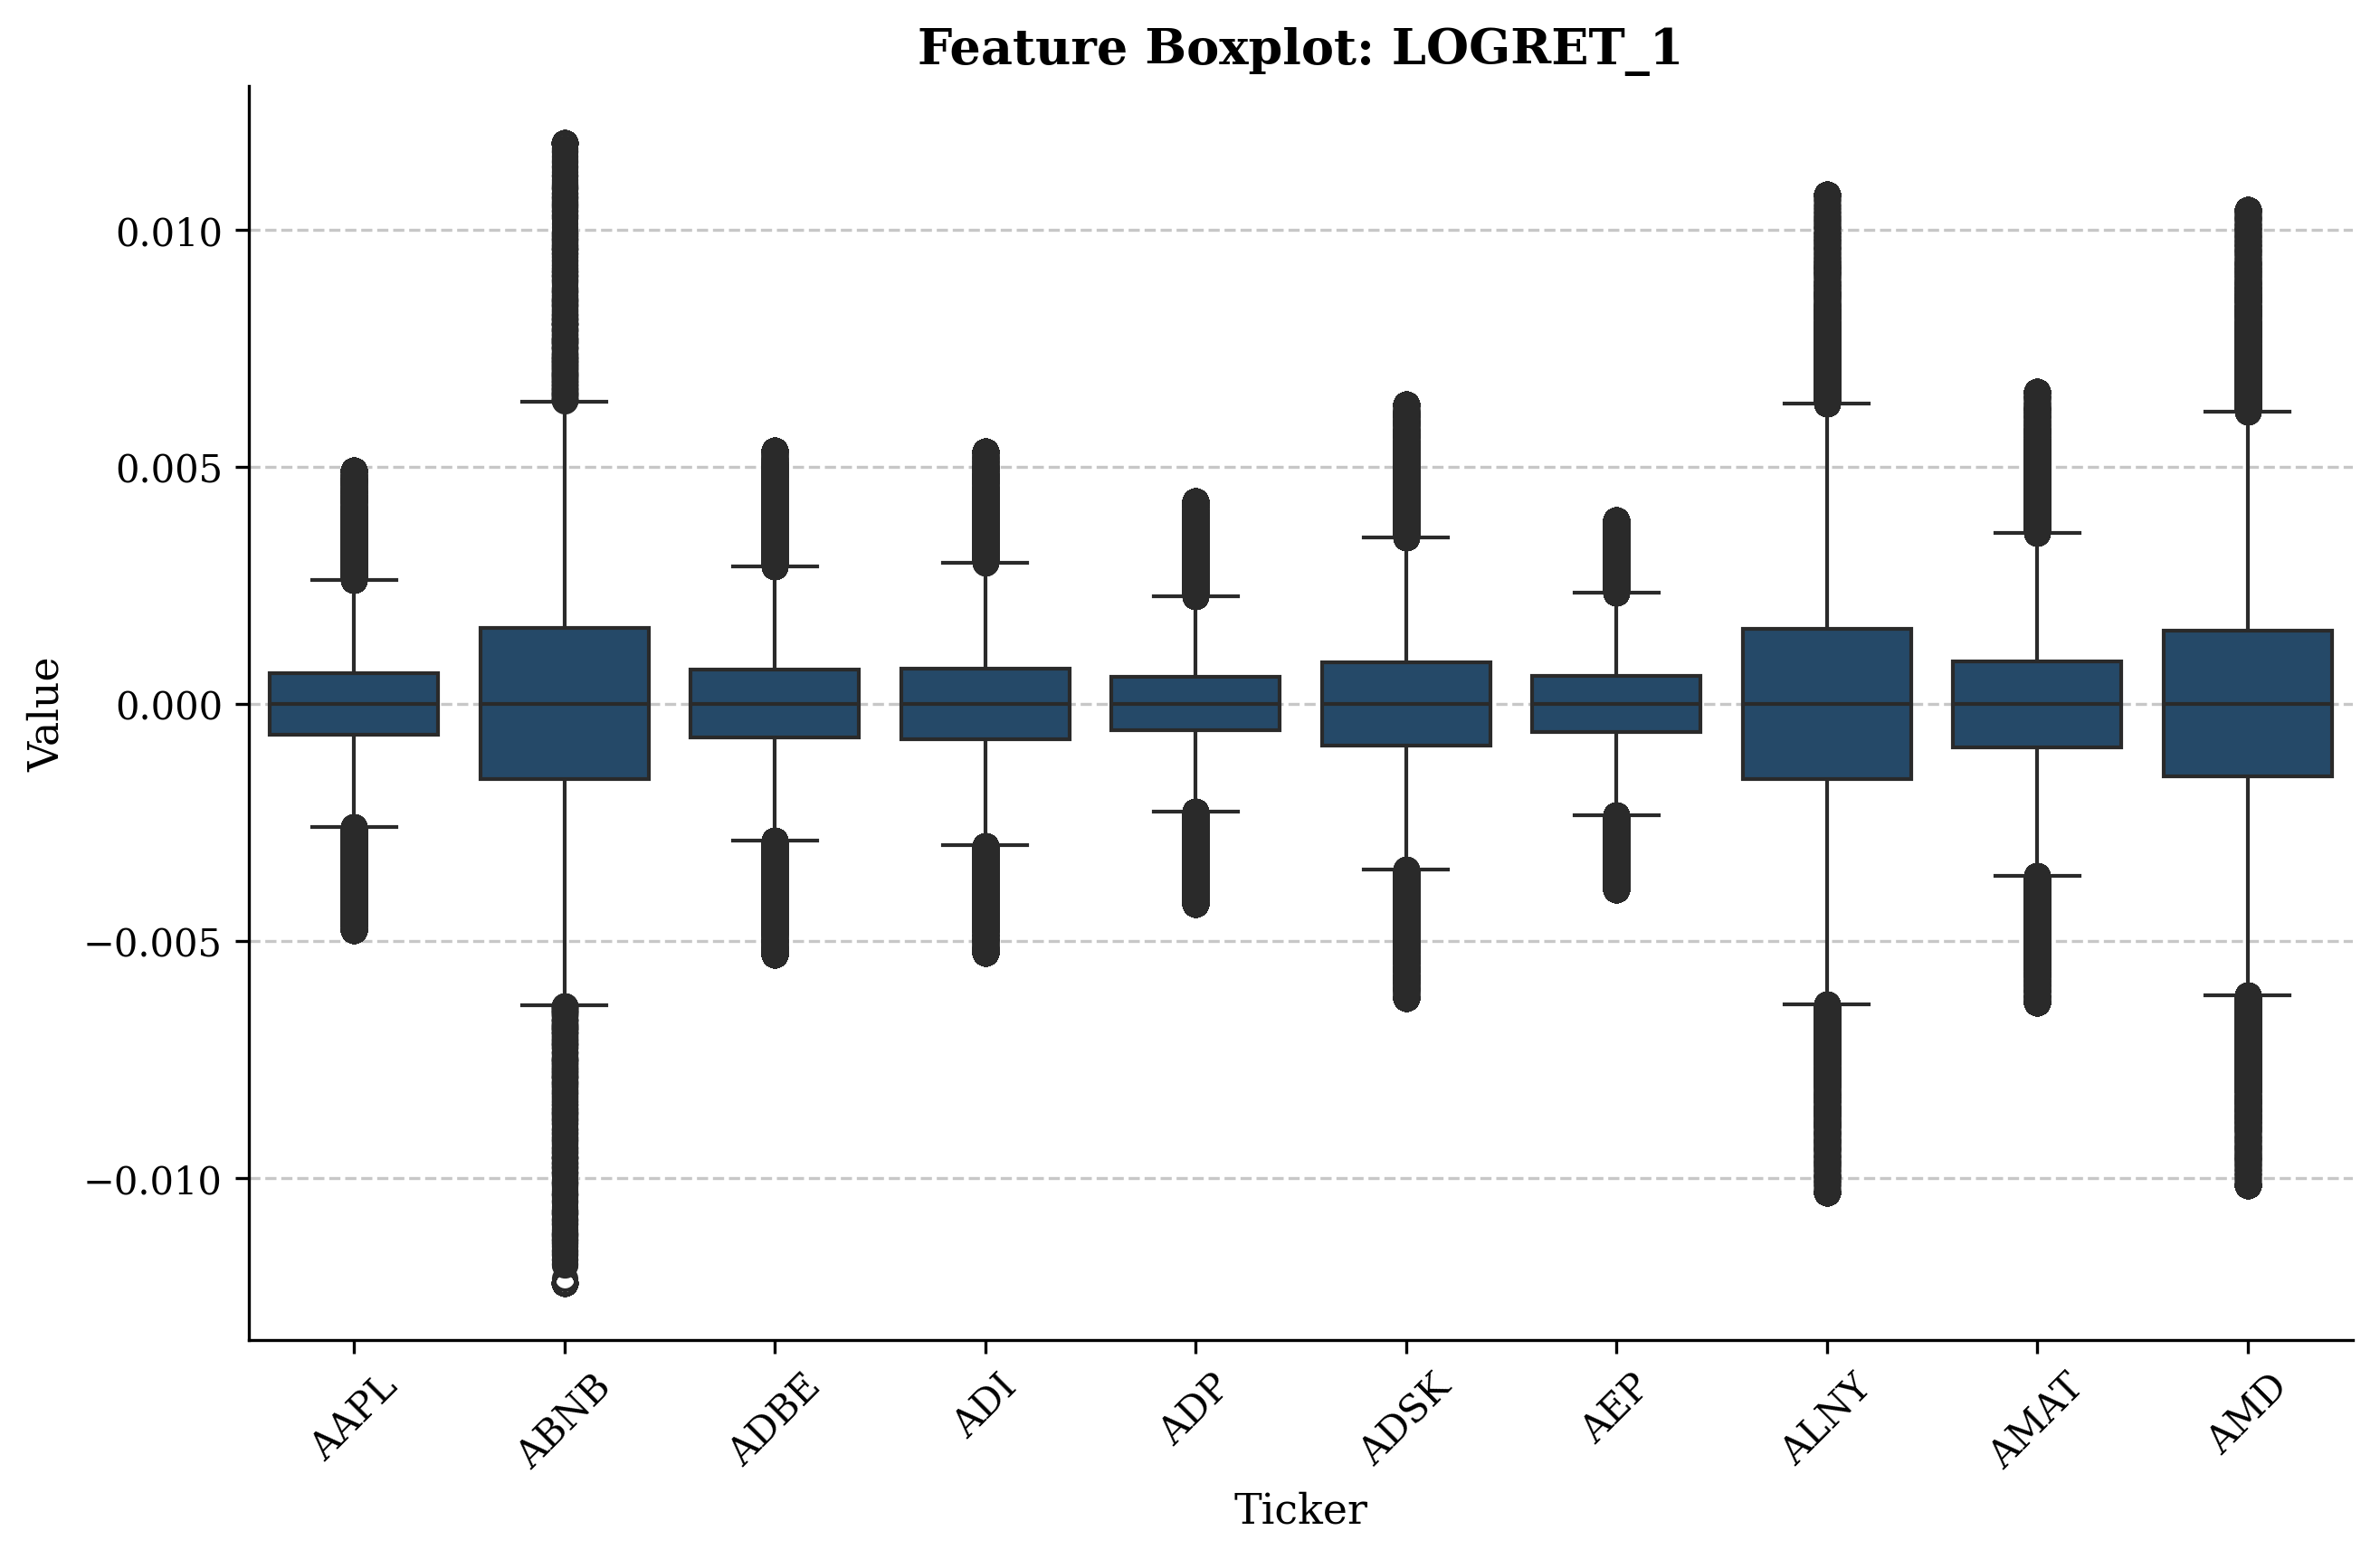
\includegraphics[width=\textwidth]{plots/boxplots/winsorized_1.0_percentiles/LOGRET_1_boxplot.png}
        \caption{Boxplot for log-return.}
        \label{fig:boxplot_winsorized_1.0_percentiles_LOGRET_1}
    \end{subfigure}
    \hfill
    \begin{subfigure}[b]{0.32\textwidth}
        \centering
        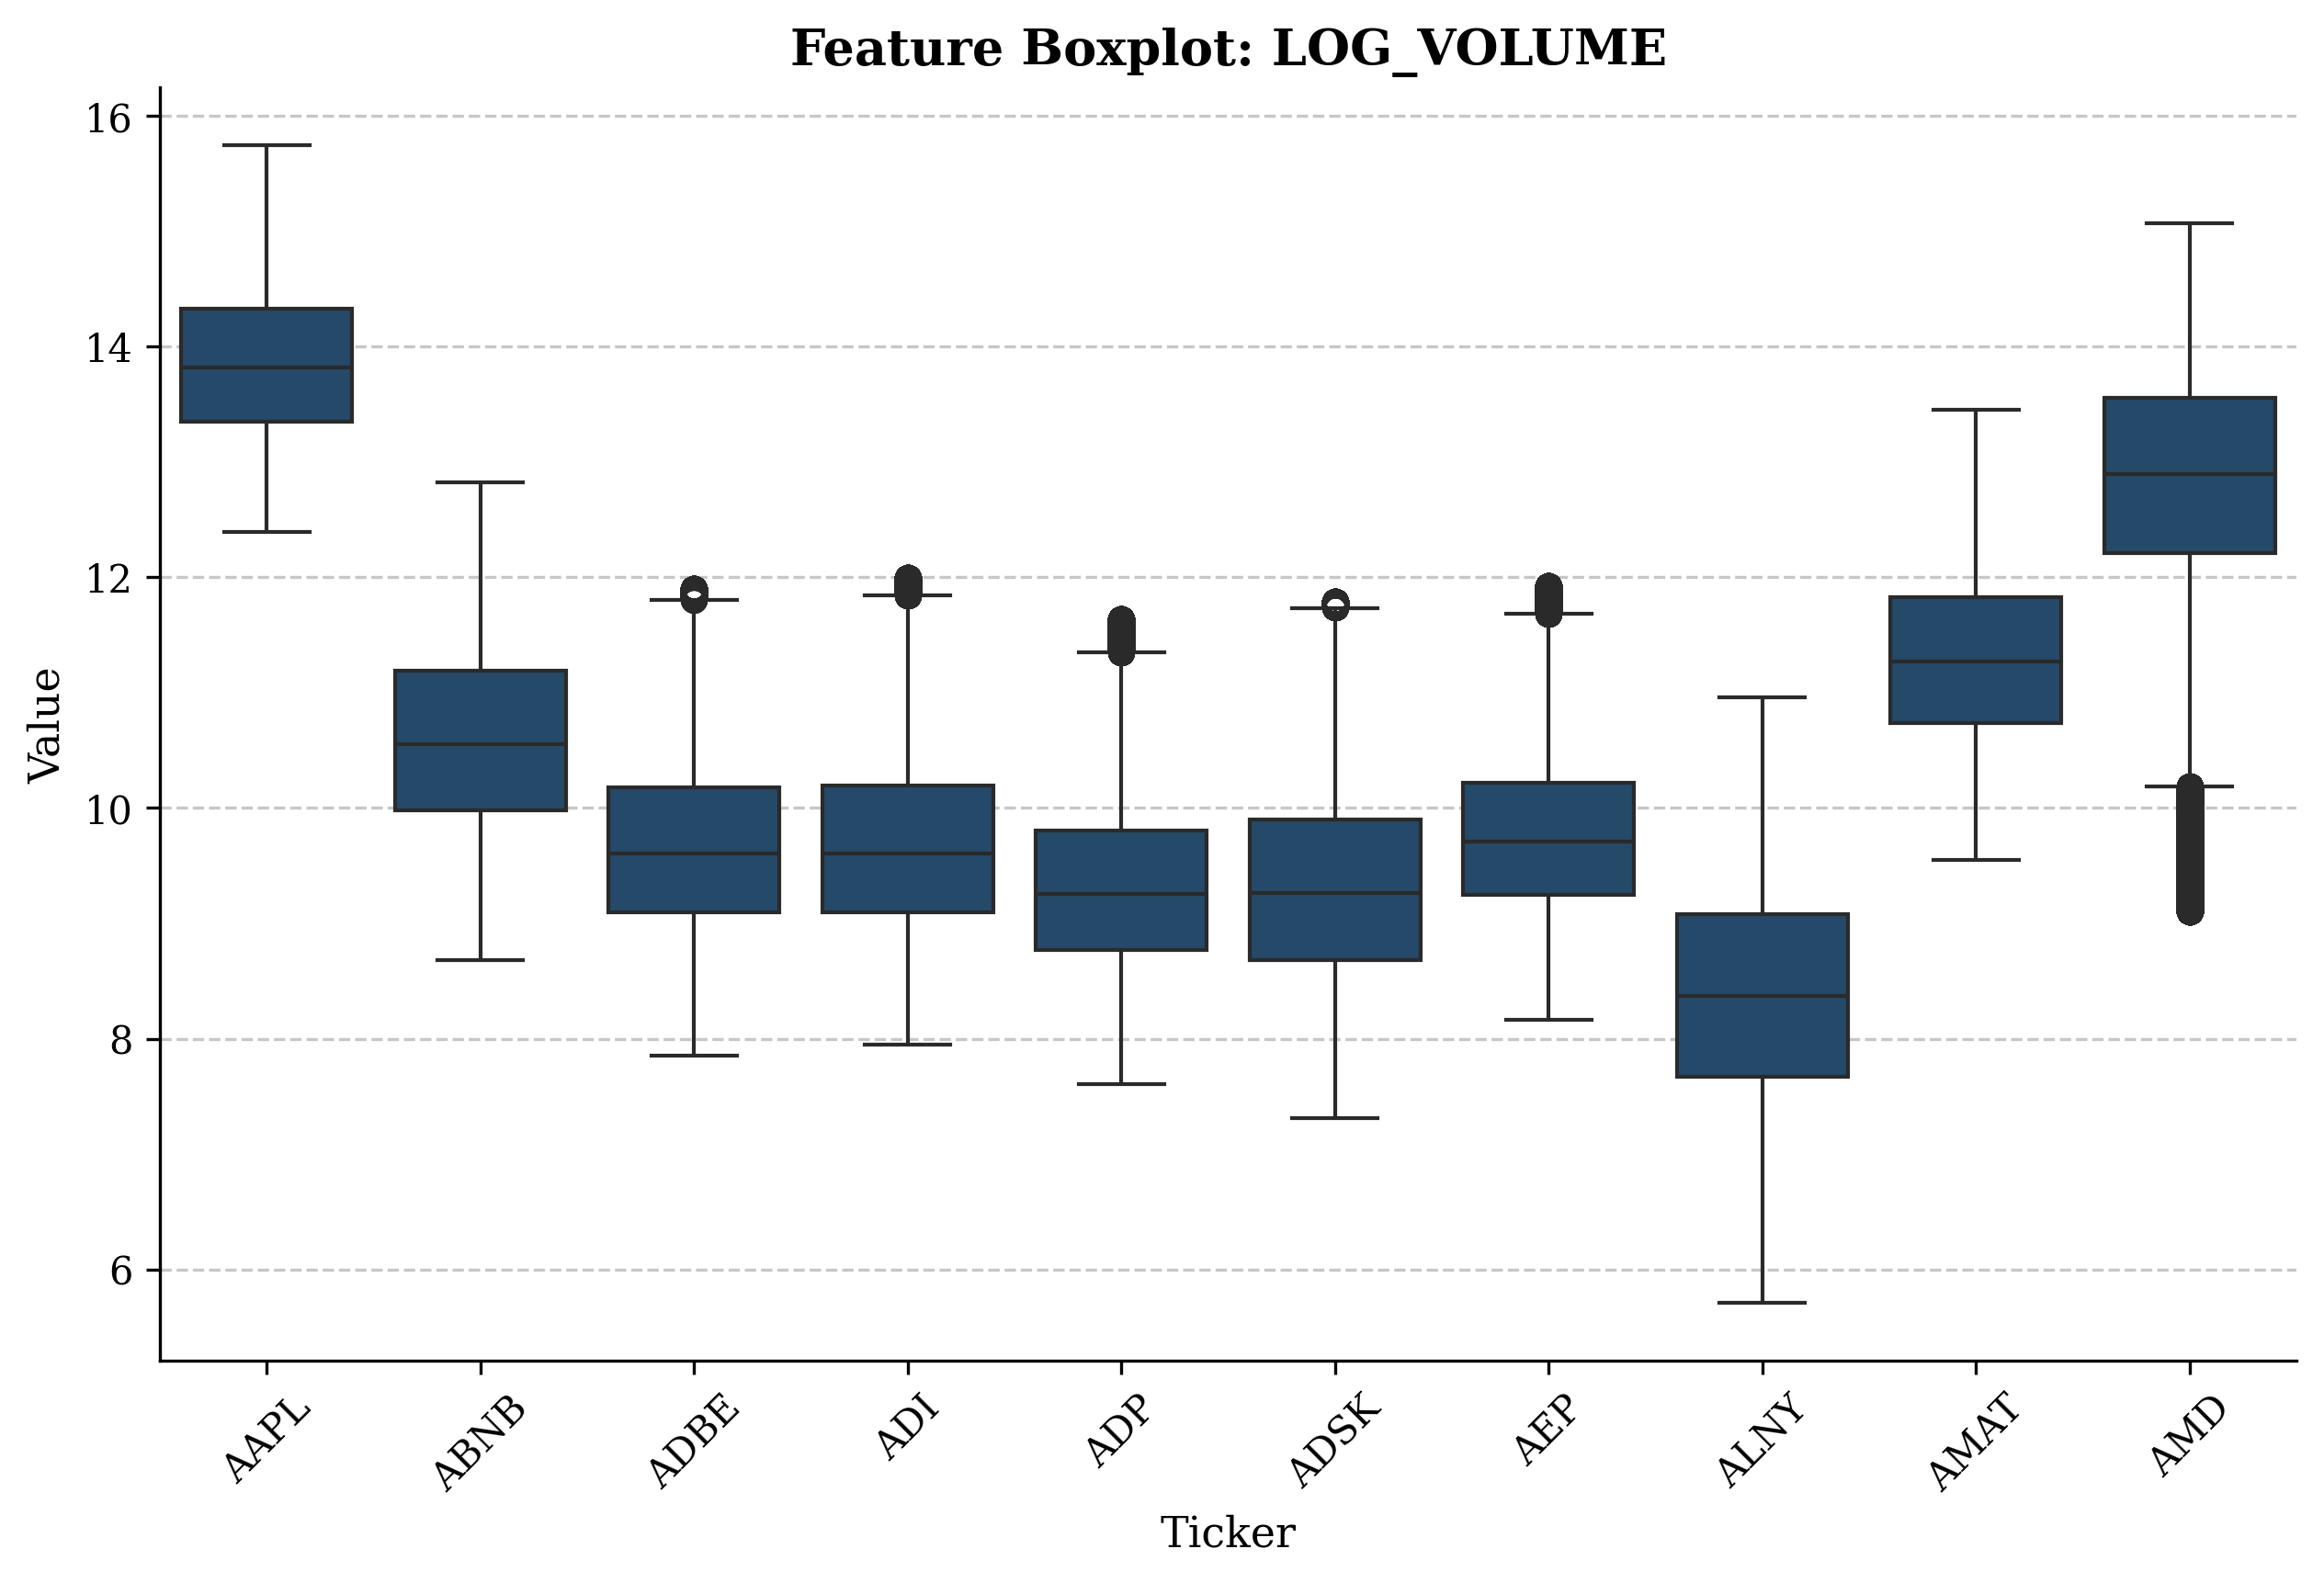
\includegraphics[width=\textwidth]{plots/boxplots/winsorized_1.0_percentiles/LOG_VOLUME_boxplot.png}
        \caption{Boxplot for log-volume.}
        \label{fig:boxplot_winsorized_1.0_percentiles_LOG_VOLUME}
    \end{subfigure}
    \hfill
    \begin{subfigure}[b]{0.32\textwidth}
        \centering
        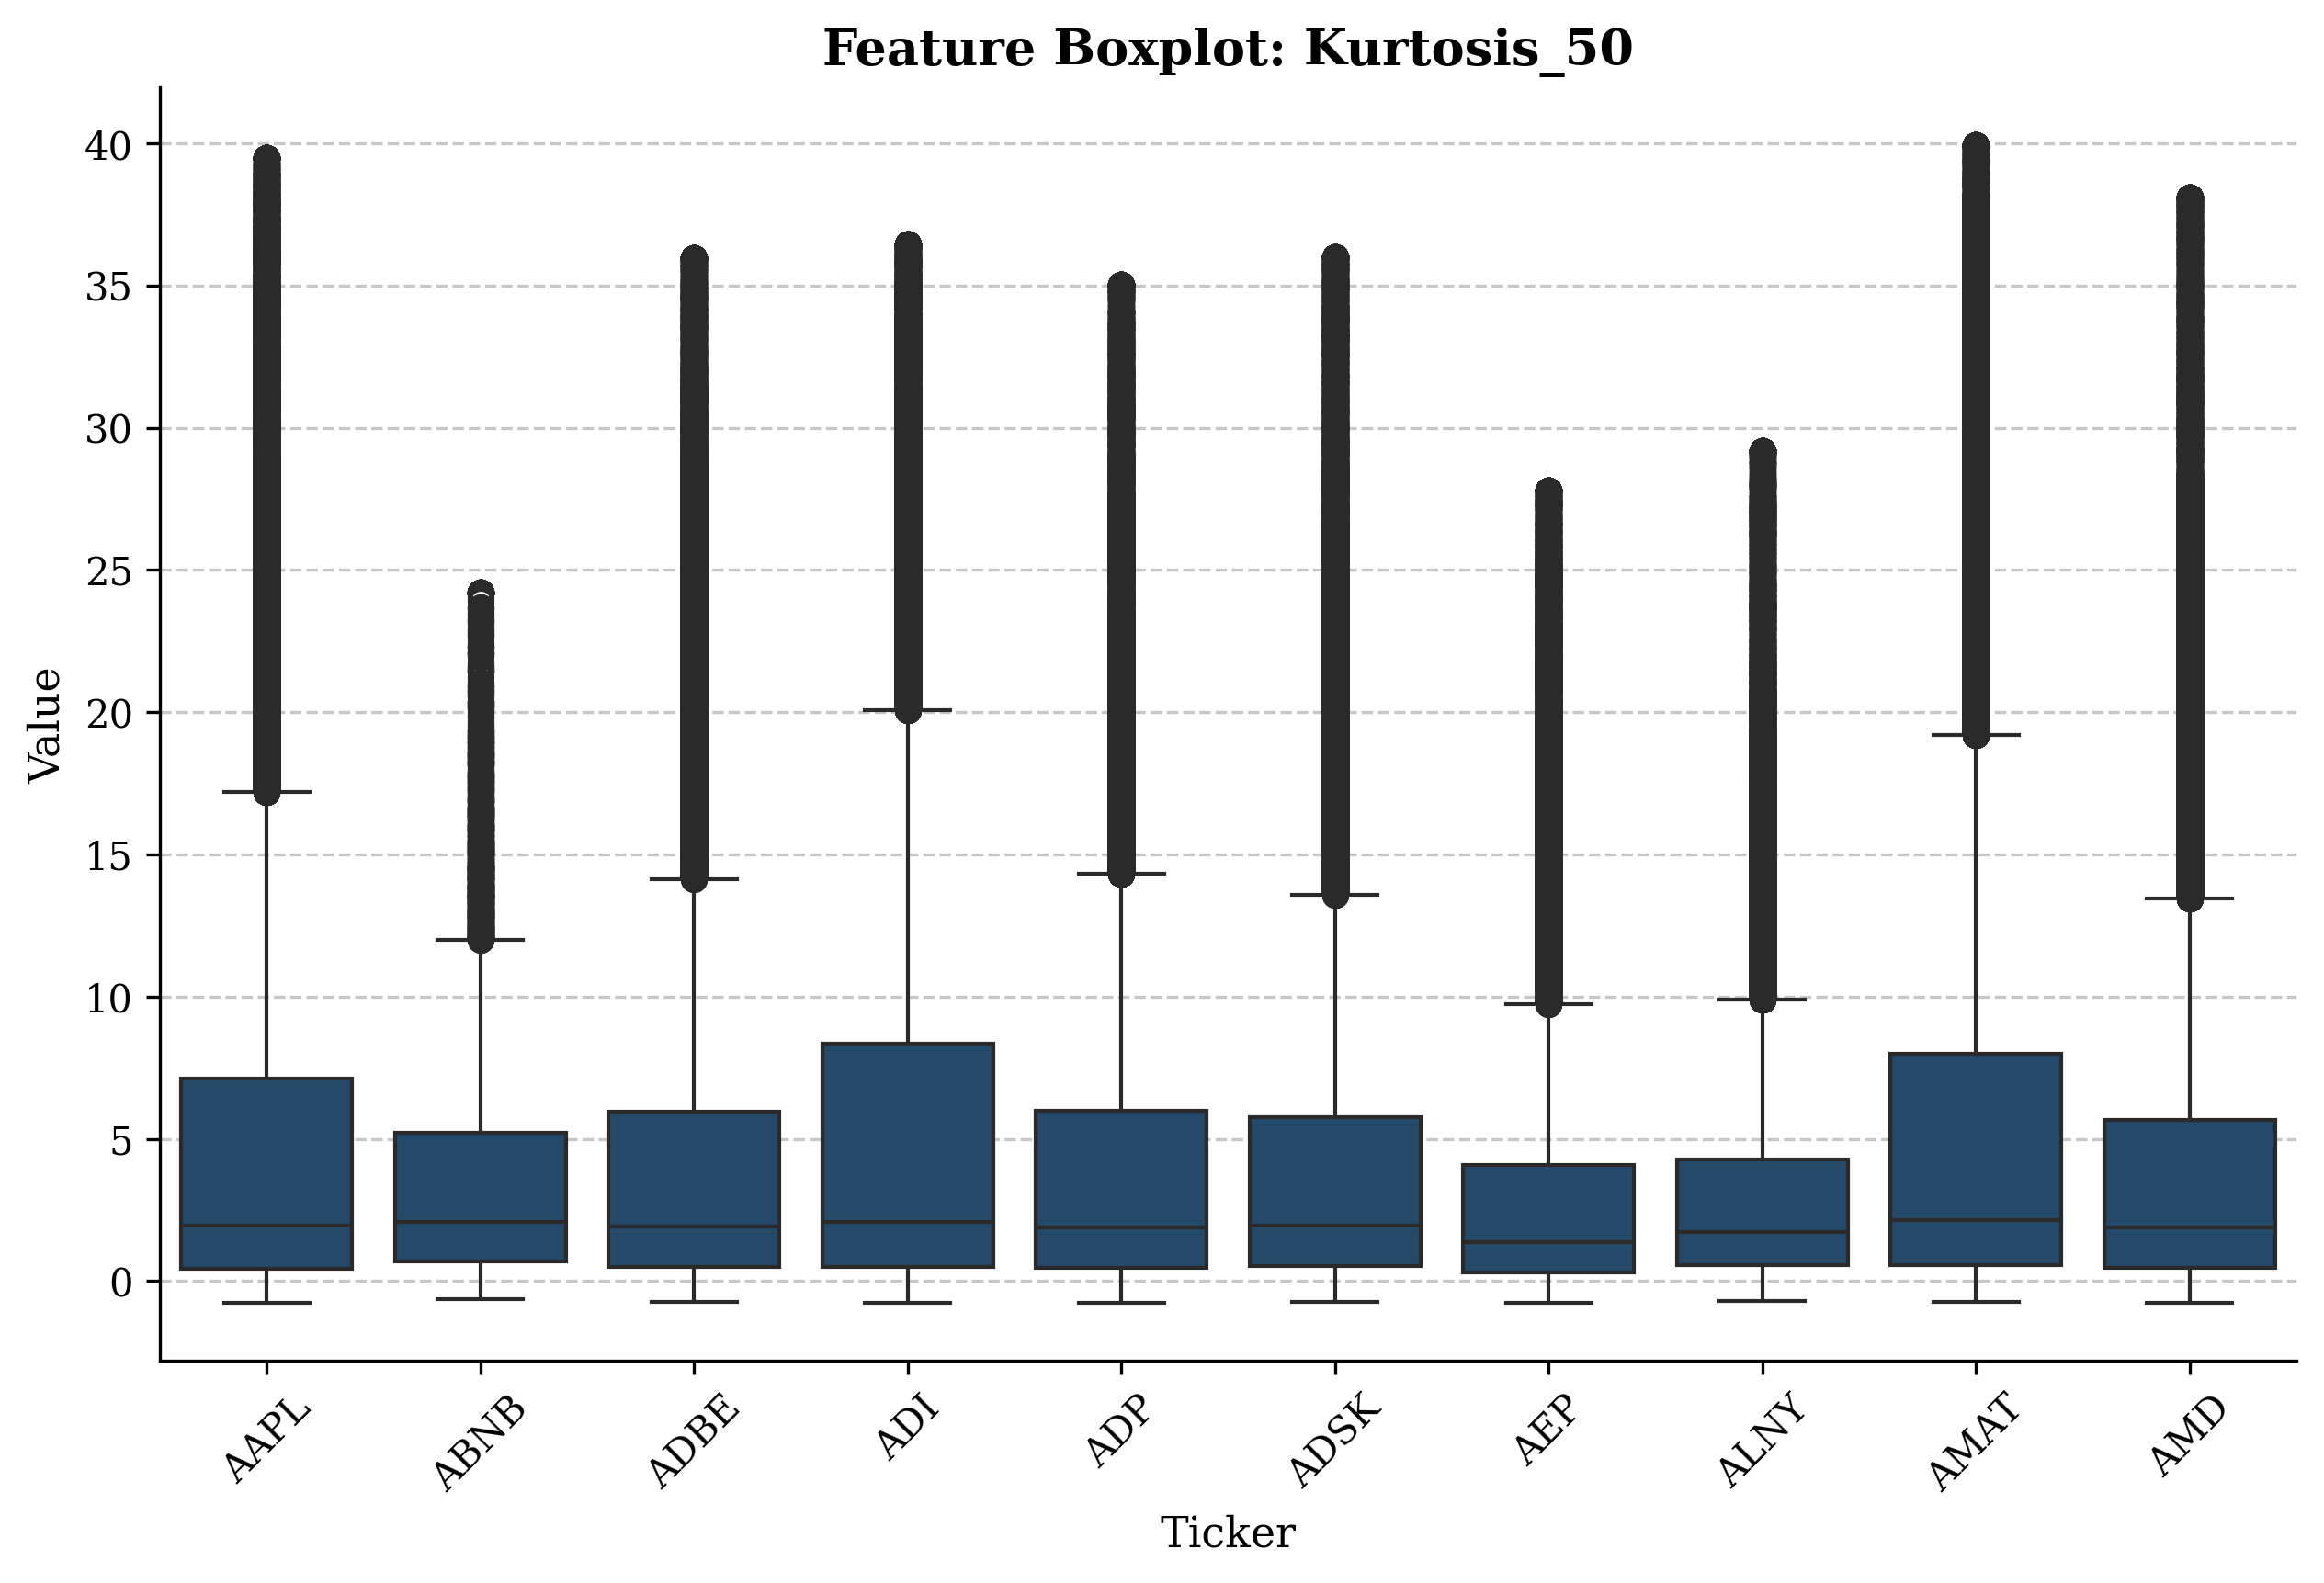
\includegraphics[width=\textwidth]{plots/boxplots/winsorized_1.0_percentiles/Kurtosis_50_boxplot.png}
        \caption{Boxplot for kurtosis.}
        \label{fig:boxplotwinsorized_1.0_percentiles_Kurtosis_50}
    \end{subfigure}

    \caption{Boxplot of winsorized features using the 1st and 99th percentiles as thresholds across 10 selected tickers. In \ref{fig:boxplot_winsorized_1.0_percentiles_LOGRET_1}, it can be  observed that the range of log-returns is reduced drastically compared to the unscaled version in Figure \ref{fig:boxplot_unscaled_LOGRET_1}. These extreme outliers have been capped at the threshold values.}
    \label{fig:boxplot_winsorized_1.0_percentiles}
\end{figure}


\subsubsection{Scaling}
The next step is to center and scale the data of each ticker $n$ respectively. A common approach in machine learning is standardization (Z-score normalization), defined as: 
\begin{equation}
    x_{\text{standard scaled}} = \frac{x - \mu}{\sigma}
\end{equation}
where $\mu$ represents the mean and $\sigma$ the standard deviation. However, as some outliers are still present even after winsorization, the mean is affected by them. It is pulled too strongly towards the extreme values. To avoid this problem, robust scaling is used. This method utilizes the median and the \gls{iqr}: 
\begin{equation}
    x_{\text{robust scaled}} = \frac{x - \text{median}}{Q_3 - Q_1}
    \label{eq:robust_scaling}
\end{equation}
Since the \gls{iqr} (the range between the 25th($Q_1$) and 75th($Q_3$) percentiles) only considers the central distribution measure, the scaling factor is significantly more stable across different market phases and volatility jumps.

It can be observed that the median for the feature kurtosis with the standard scaling method is distorted more into the negative direction compared to the robust scaling method (see Figure \ref{fig:boxplot_standardscaled_winsorized_1.0_percentiles_Kurtosis_50}). This is the result of the still present positive outliers. 

\begin{figure}[htbp]
    \centering
    \begin{subfigure}[b]{0.32\textwidth}
        \centering
        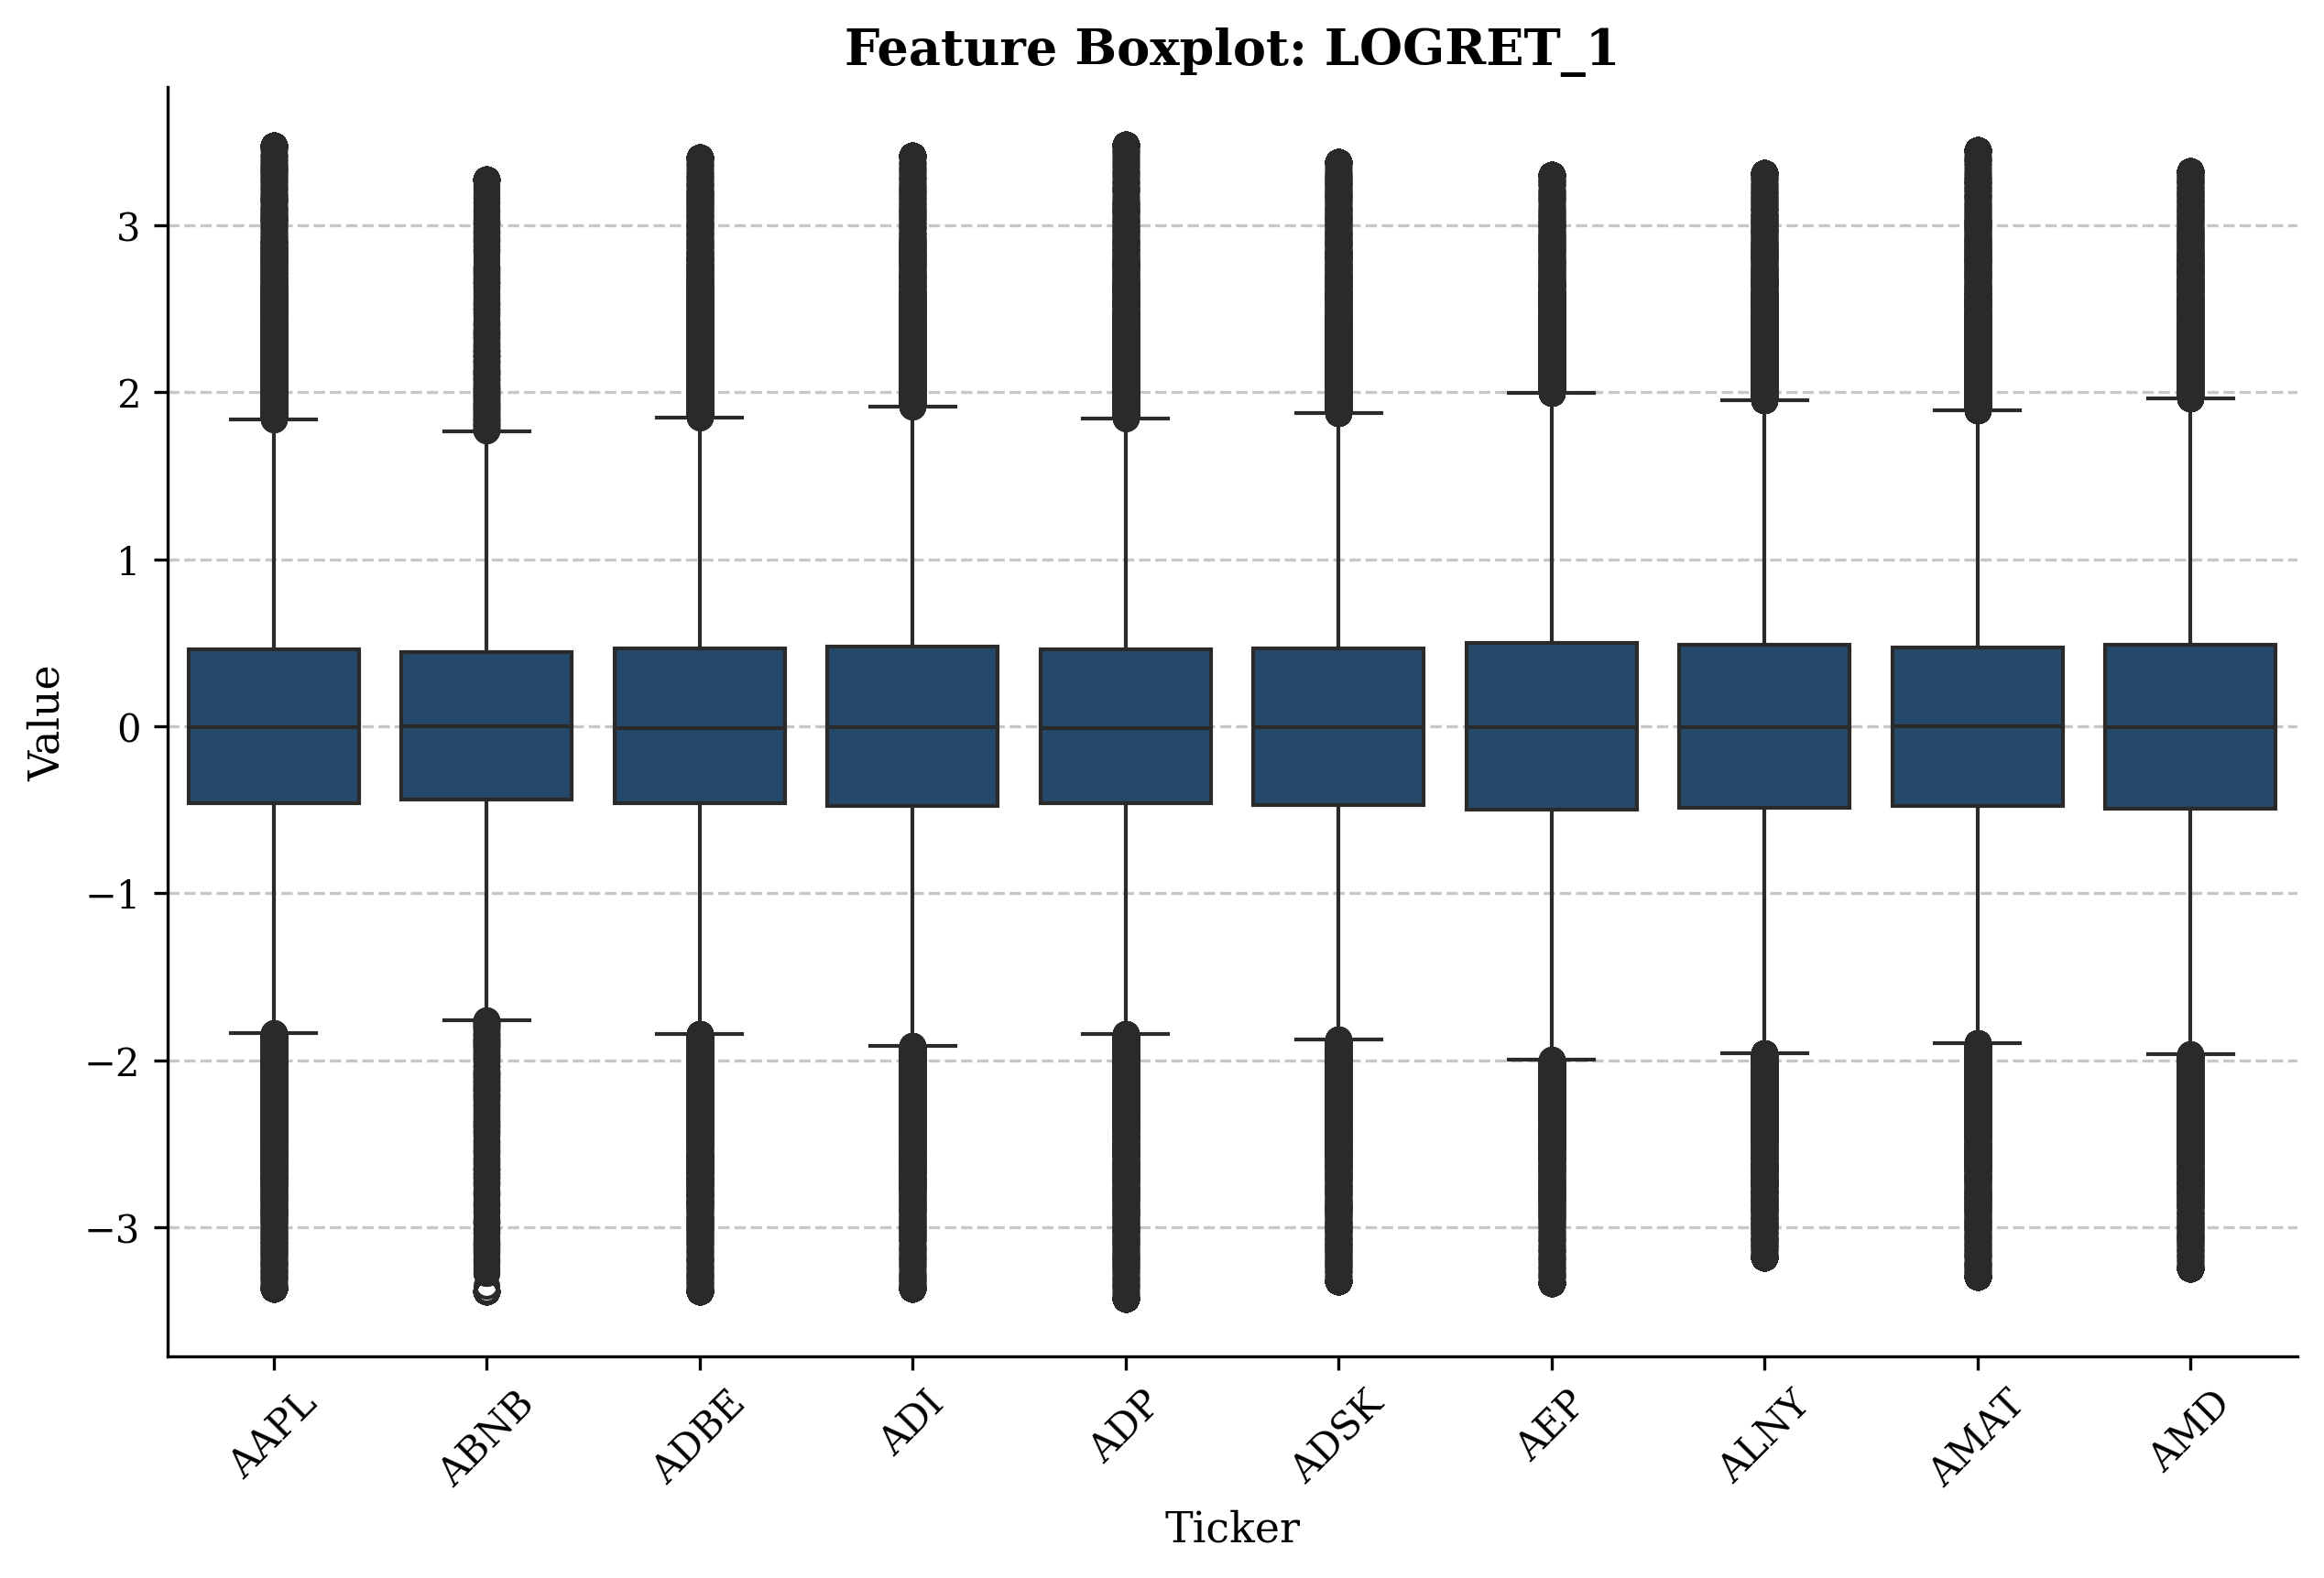
\includegraphics[width=\textwidth]{plots/boxplots/standardscaled_winsorized_1.0_percentiles/LOGRET_1_boxplot.png}
        \caption{Boxplot for log-return.}
        \label{fig:boxplot_standardscaled_winsorized_1.0_percentiles_LOGRET_1}
    \end{subfigure}
    \hfill
    \begin{subfigure}[b]{0.32\textwidth}
        \centering
        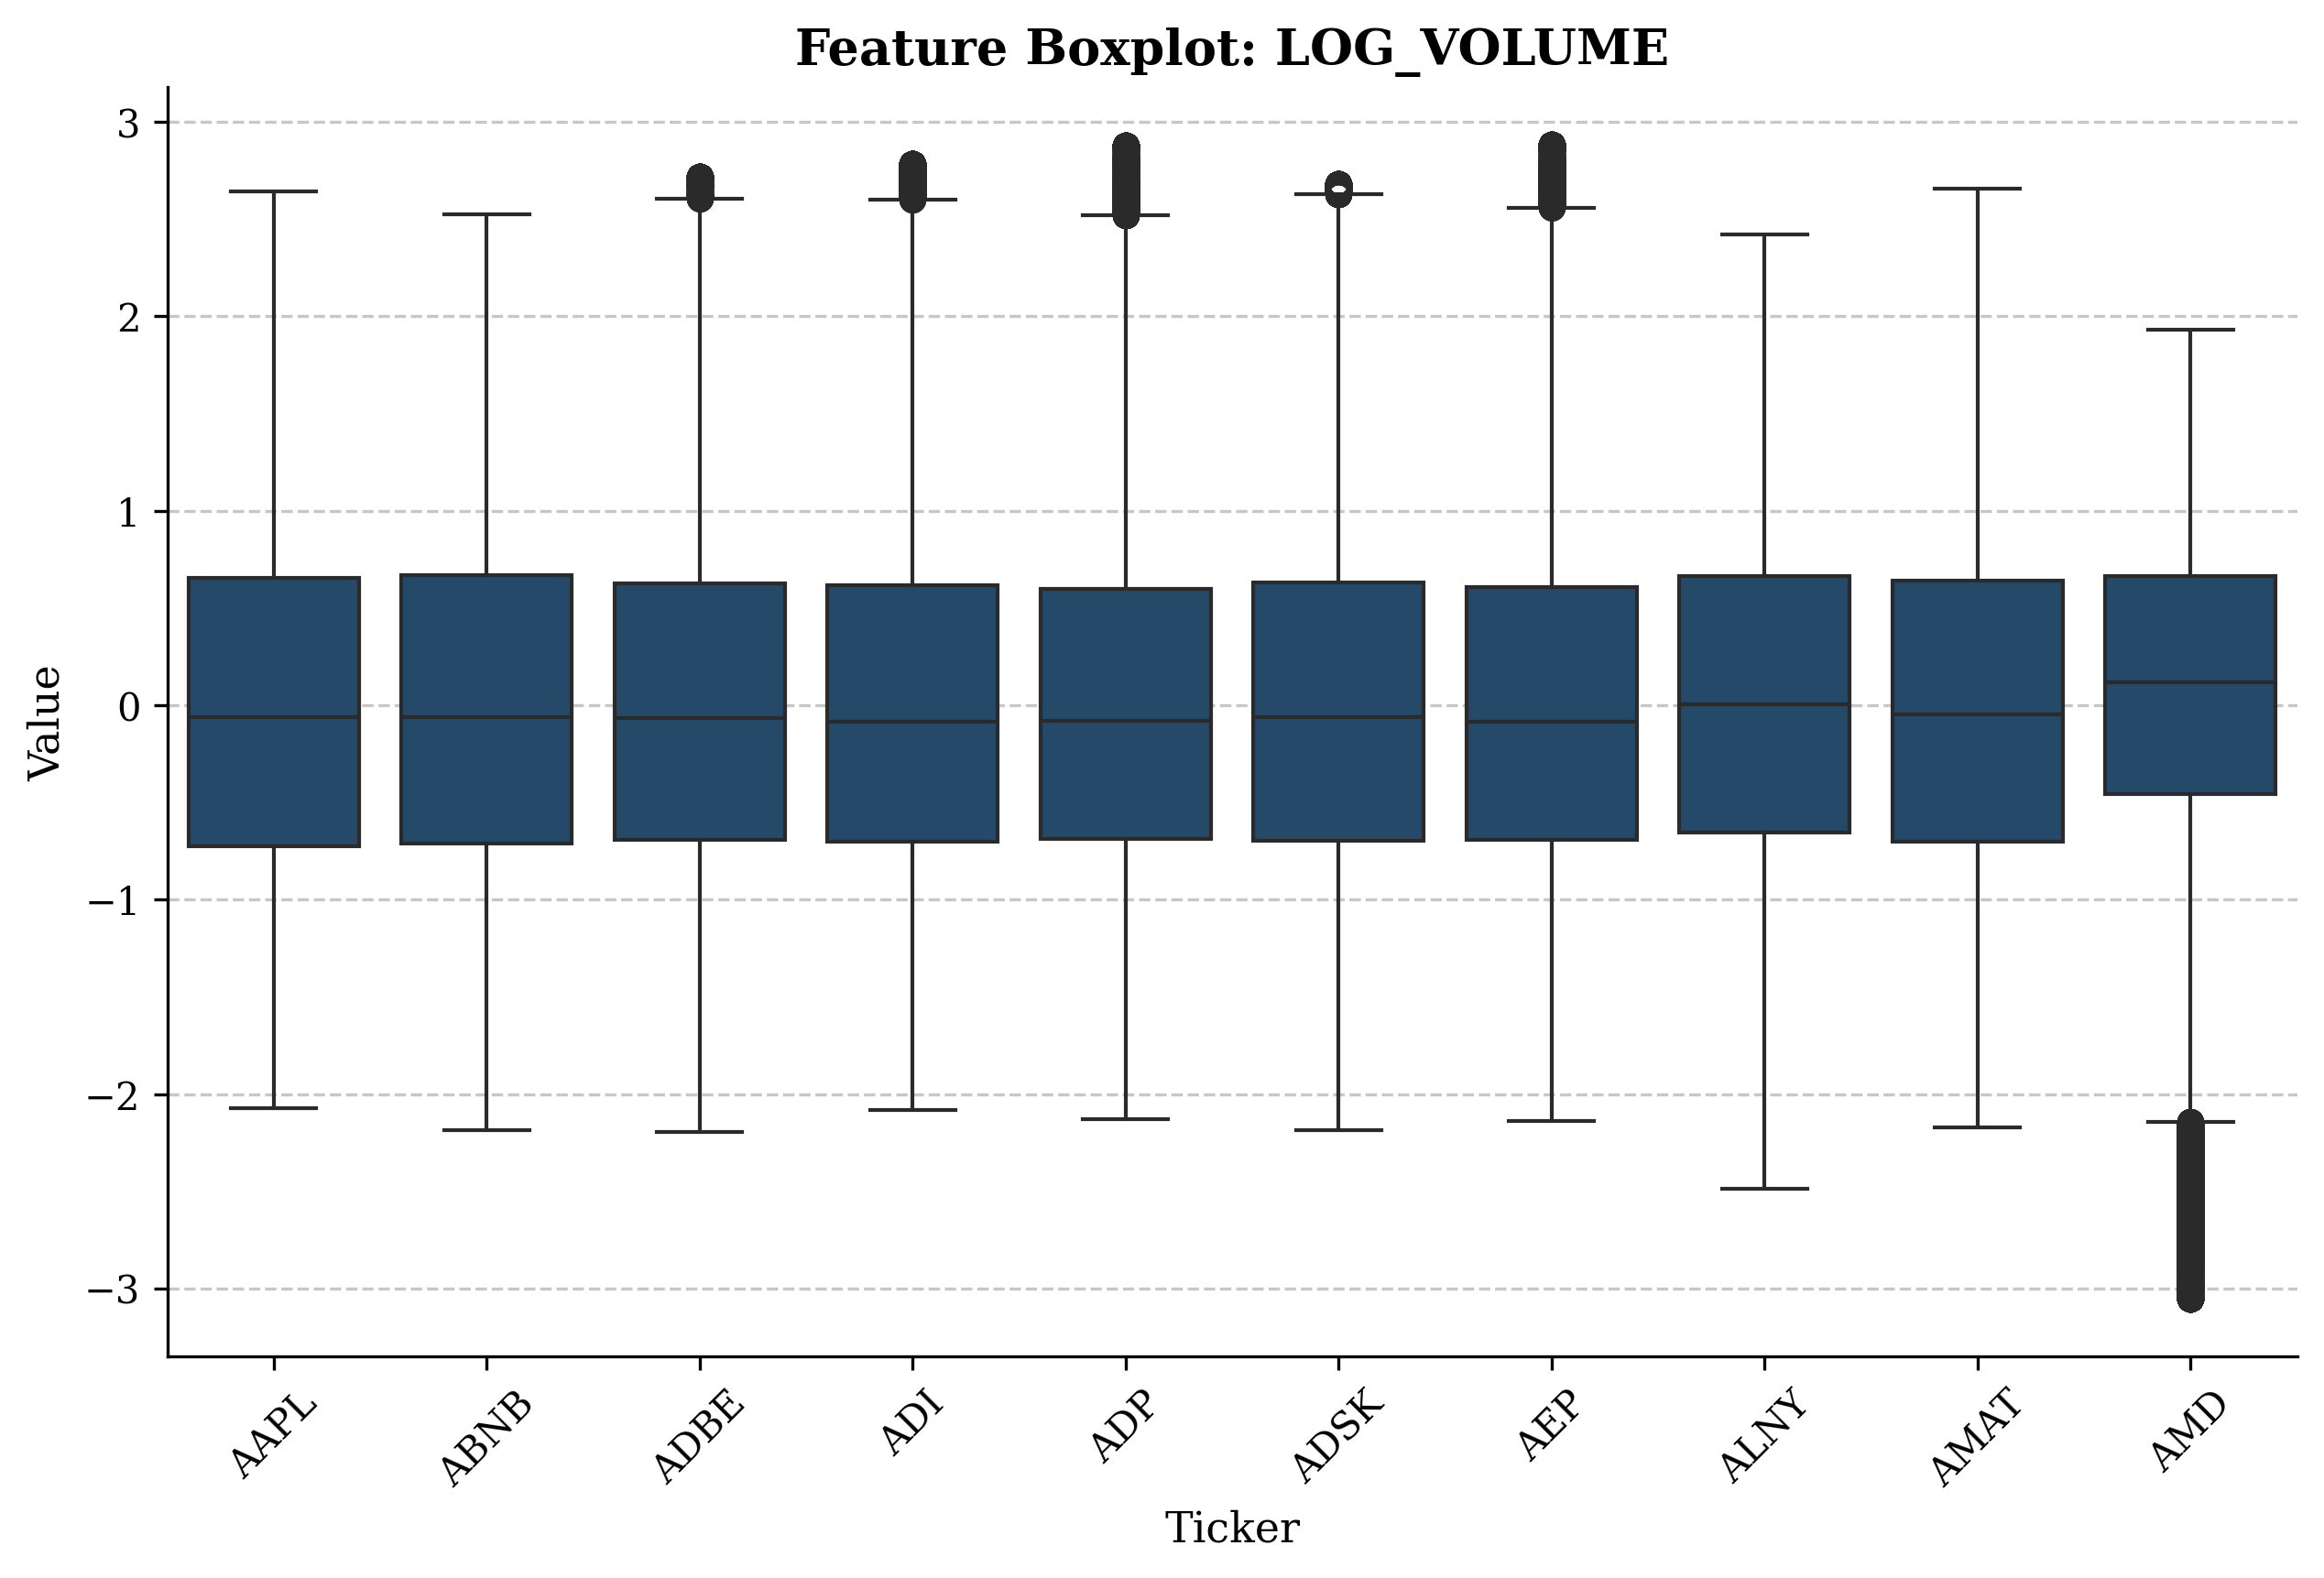
\includegraphics[width=\textwidth]{plots/boxplots/standardscaled_winsorized_1.0_percentiles/LOG_VOLUME_boxplot.png}
        \caption{Boxplot for log-volume}
        \label{fig:boxplot_standardscaled_winsorized_1.0_percentiles_LOG_VOLUME}
    \end{subfigure}
    \hfill
    \begin{subfigure}[b]{0.32\textwidth}
        \centering
        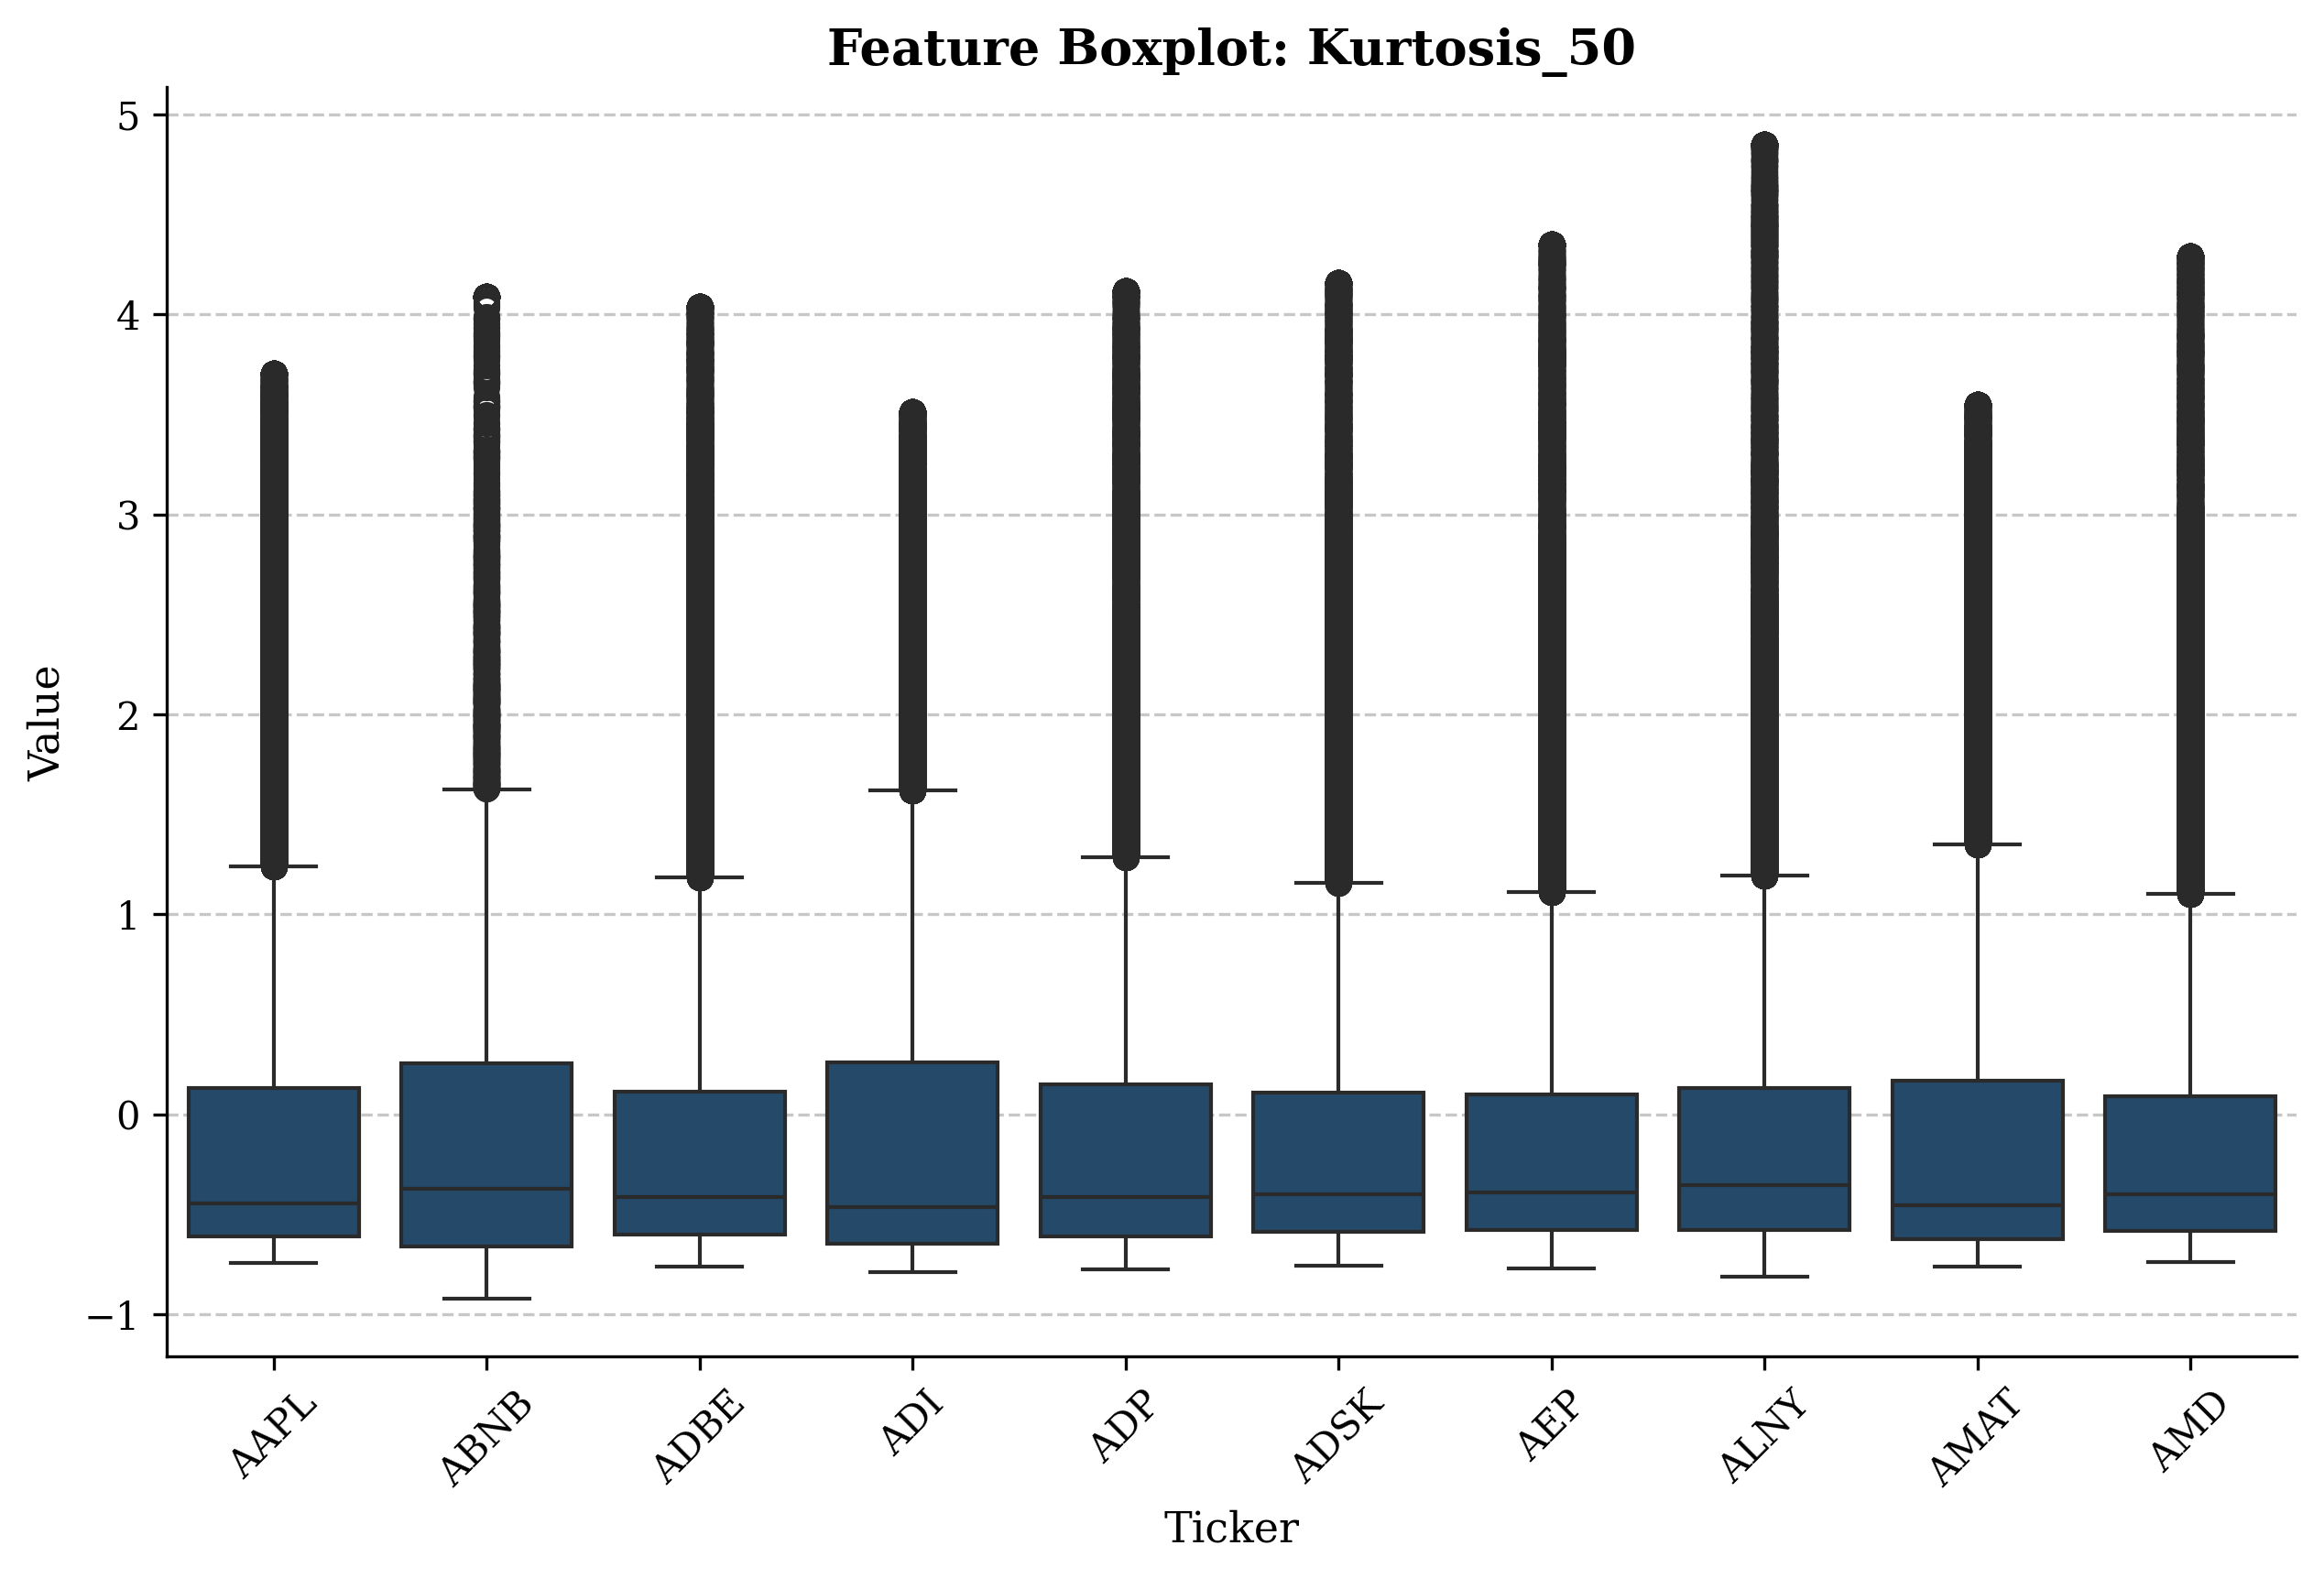
\includegraphics[width=\textwidth]{plots/boxplots/standardscaled_winsorized_1.0_percentiles/Kurtosis_50_boxplot.png}
        \caption{Boxplot for kurtosis}
        \label{fig:boxplot_standardscaled_winsorized_1.0_percentiles_Kurtosis_50}
    \end{subfigure}

    \caption{Boxplot of data that was first winsorized and then scaled with the standard scaling method on selected tickers.}
    \label{fig:boxplot_standardscaled_winsorized_1.0_percentiles}
\end{figure}


\begin{figure}[htbp]
    \centering
    \begin{subfigure}[b]{0.32\textwidth}
        \centering
        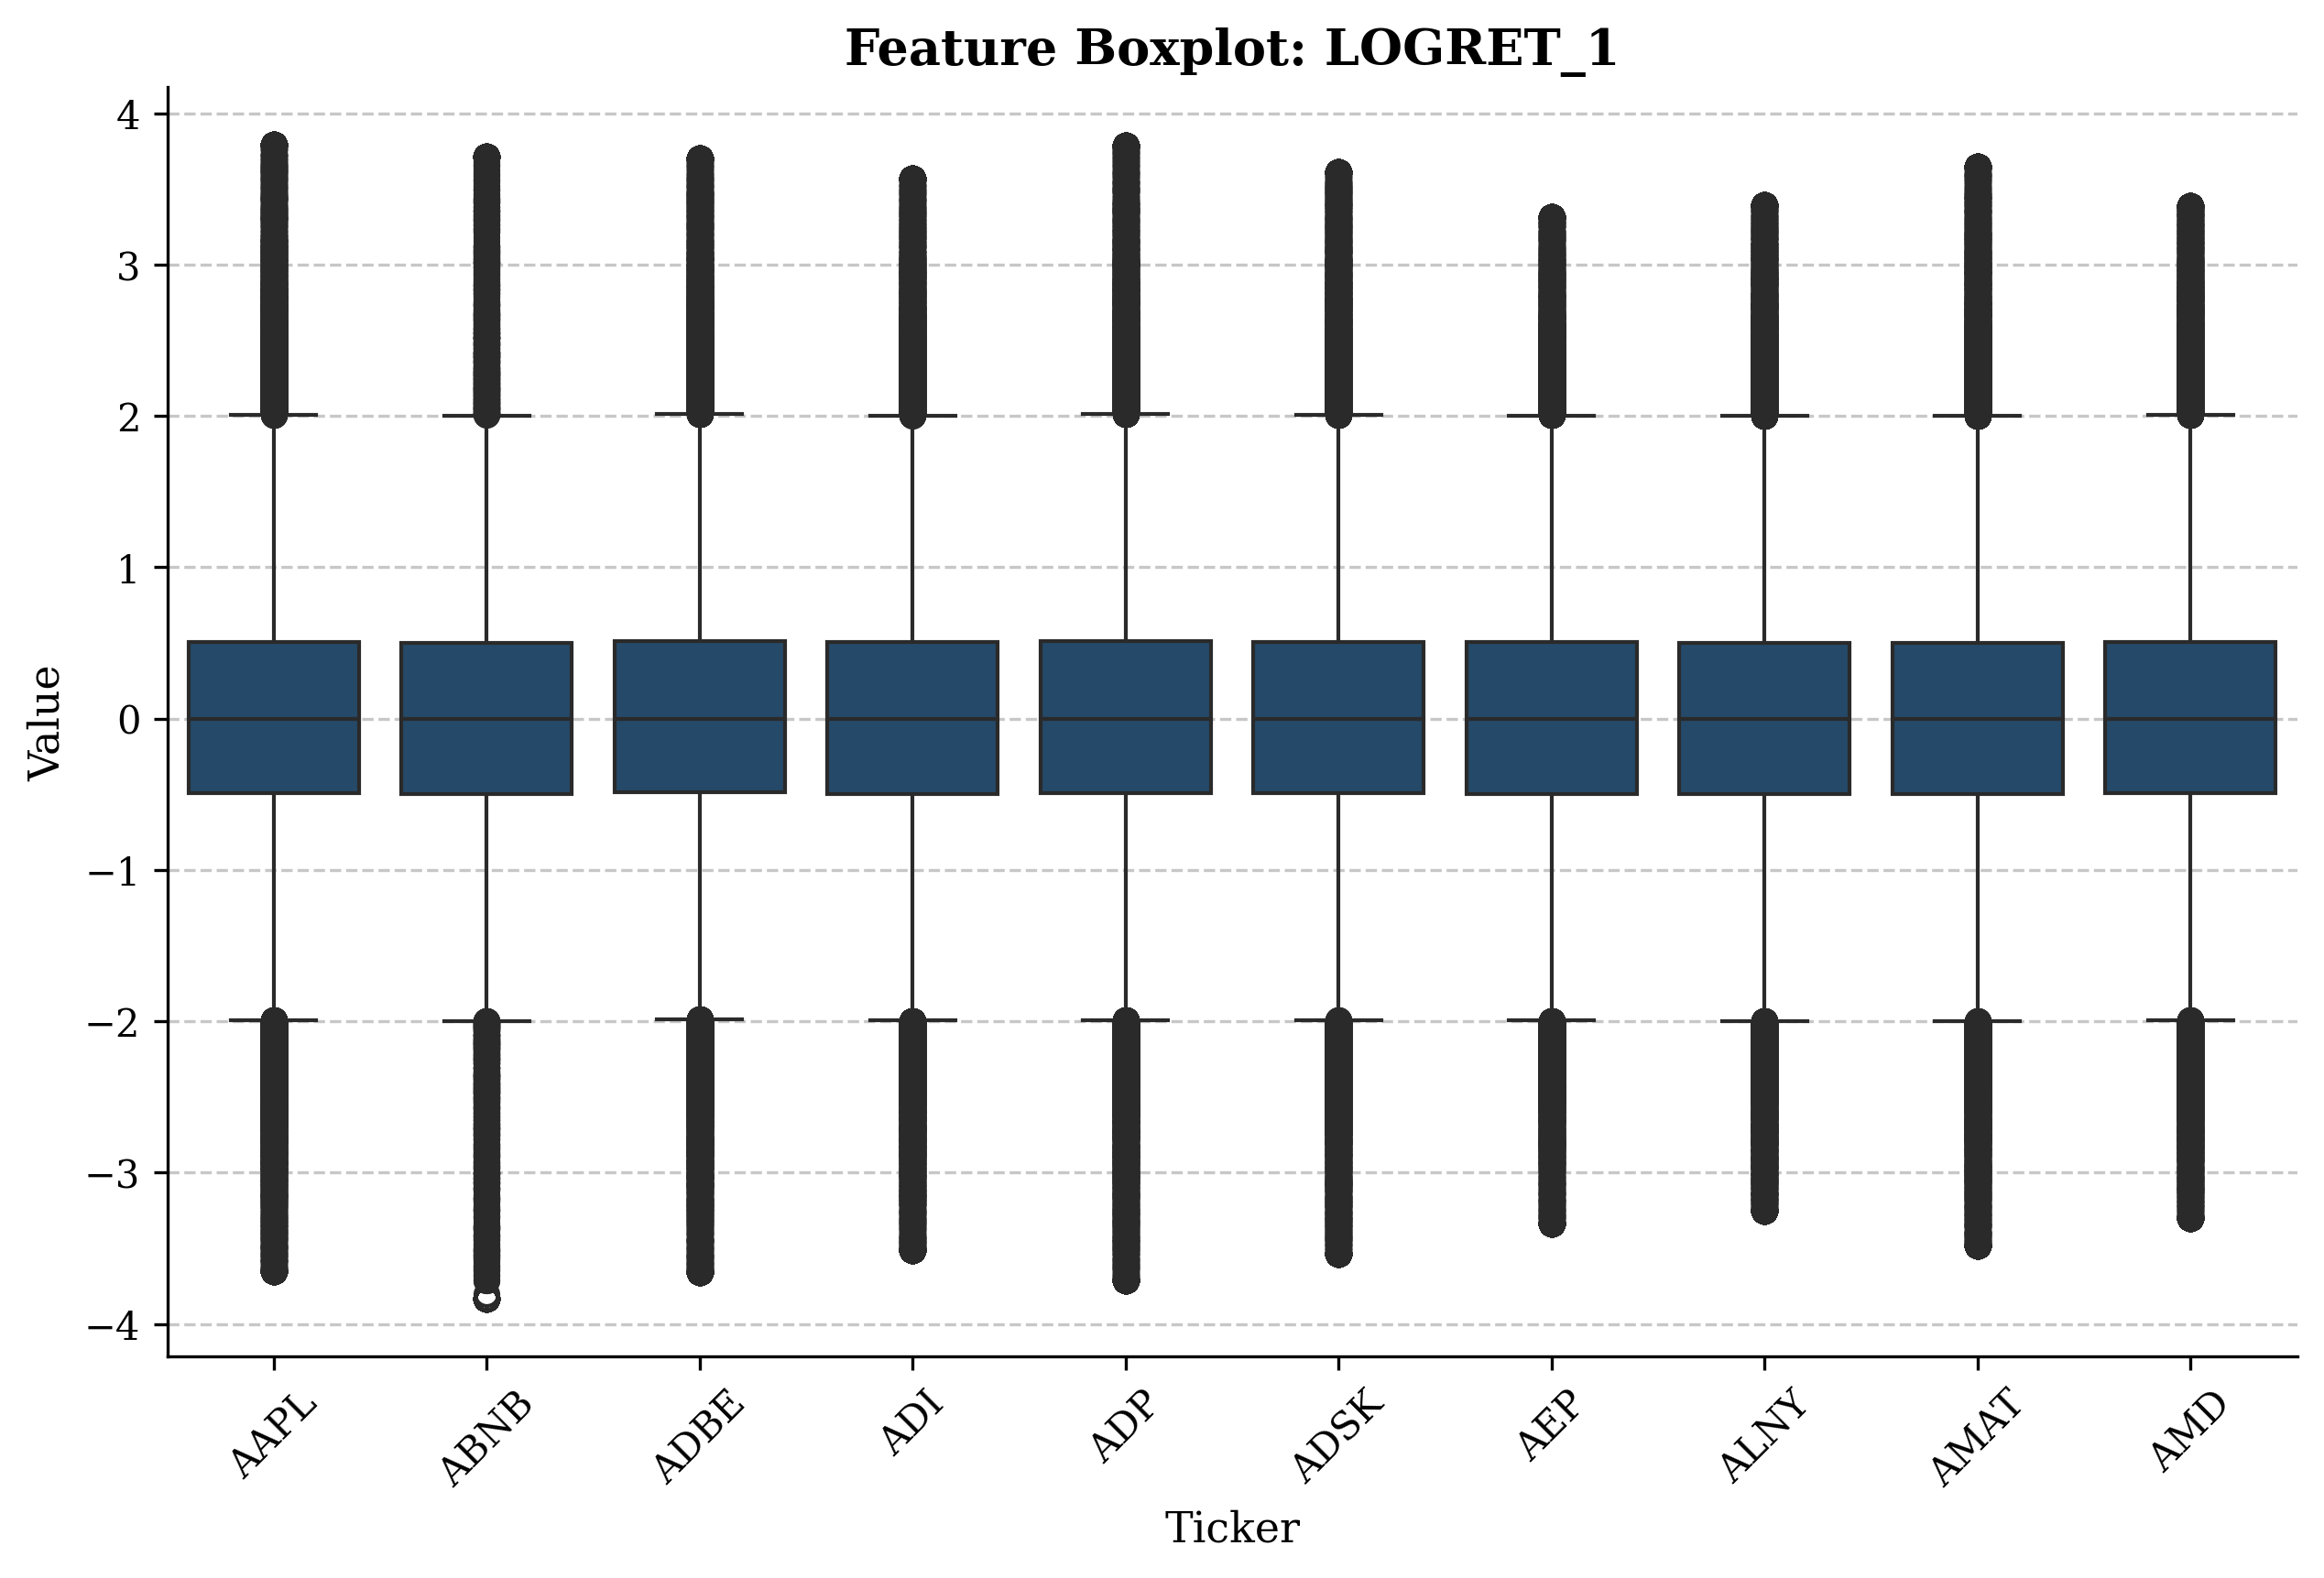
\includegraphics[width=\textwidth]{plots/boxplots/robustscaled_winsorized_1.0_percentiles/LOGRET_1_boxplot.png}
        \caption{Boxplot for log-return.}
        \label{fig:boxplot_robustscaled_winsorized_1.0_percentiles_LOGRET_1}
    \end{subfigure}
    \hfill
    \begin{subfigure}[b]{0.32\textwidth}
        \centering
        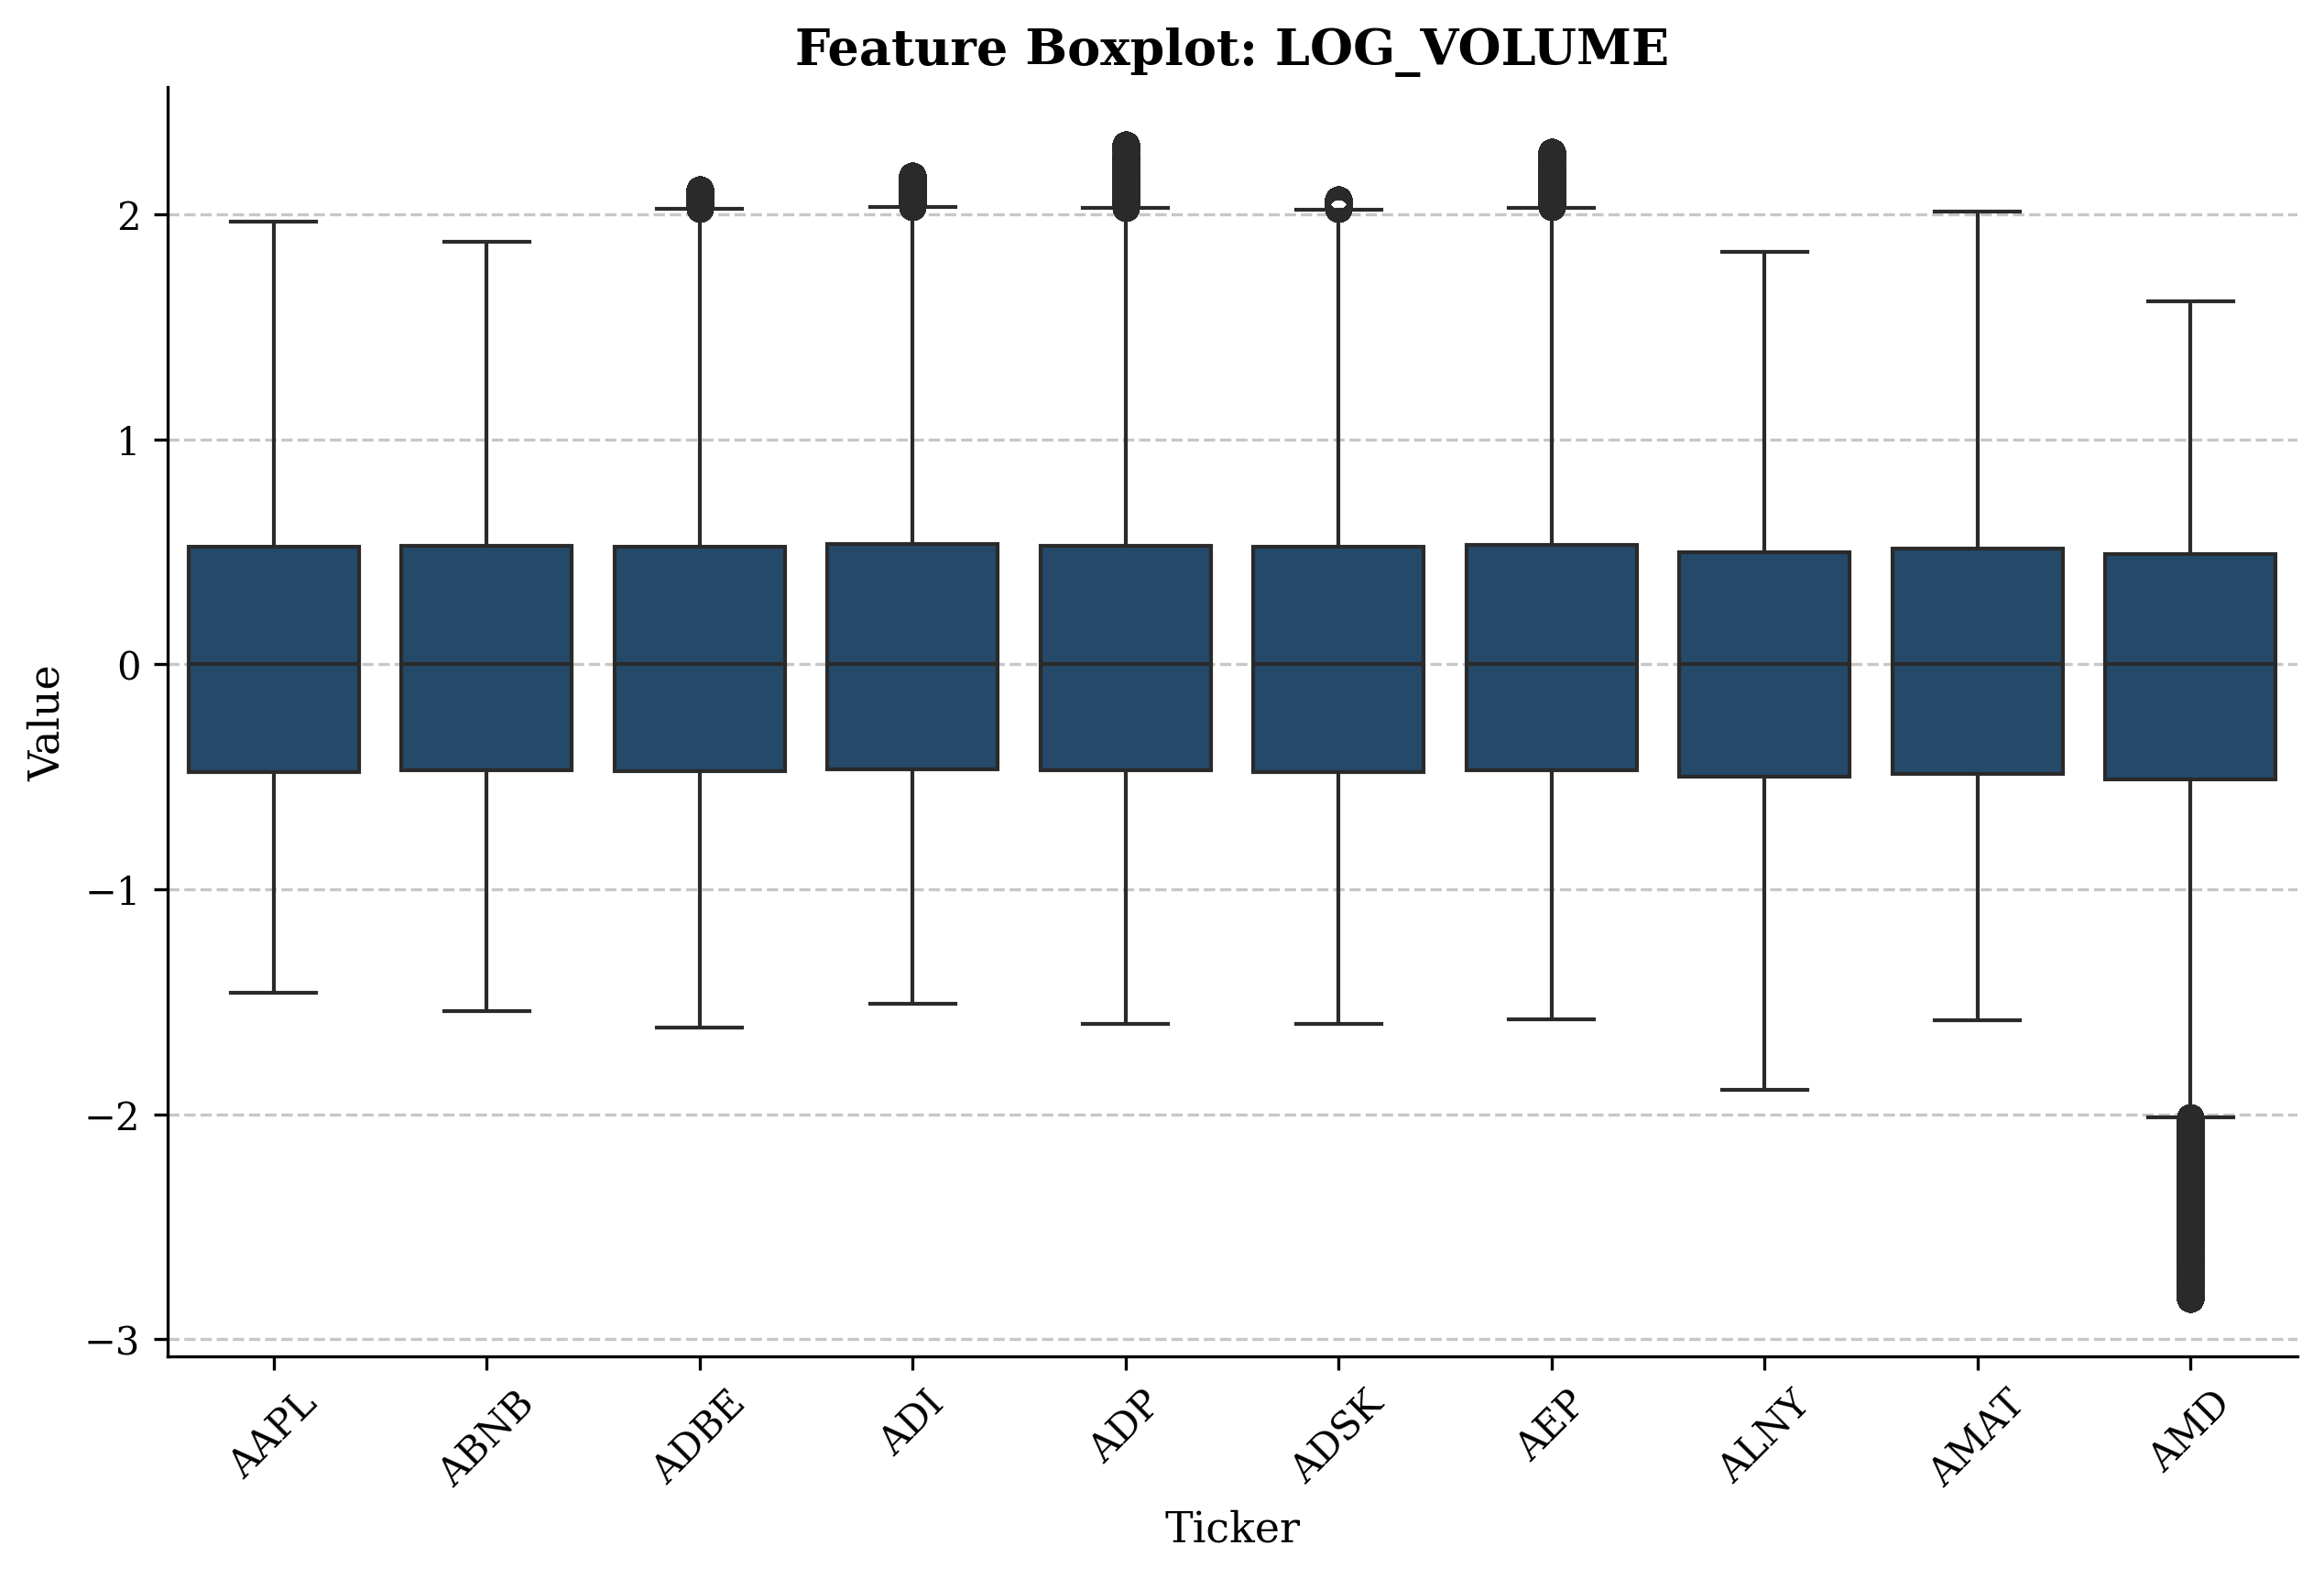
\includegraphics[width=\textwidth]{plots/boxplots/robustscaled_winsorized_1.0_percentiles/LOG_VOLUME_boxplot.png}
        \caption{Boxplot for log-volume}
        \label{fig:boxplot_robustscaled_winsorized_1.0_percentiles_LOG_VOLUME}
    \end{subfigure}
    \hfill
    \begin{subfigure}[b]{0.32\textwidth}
        \centering
        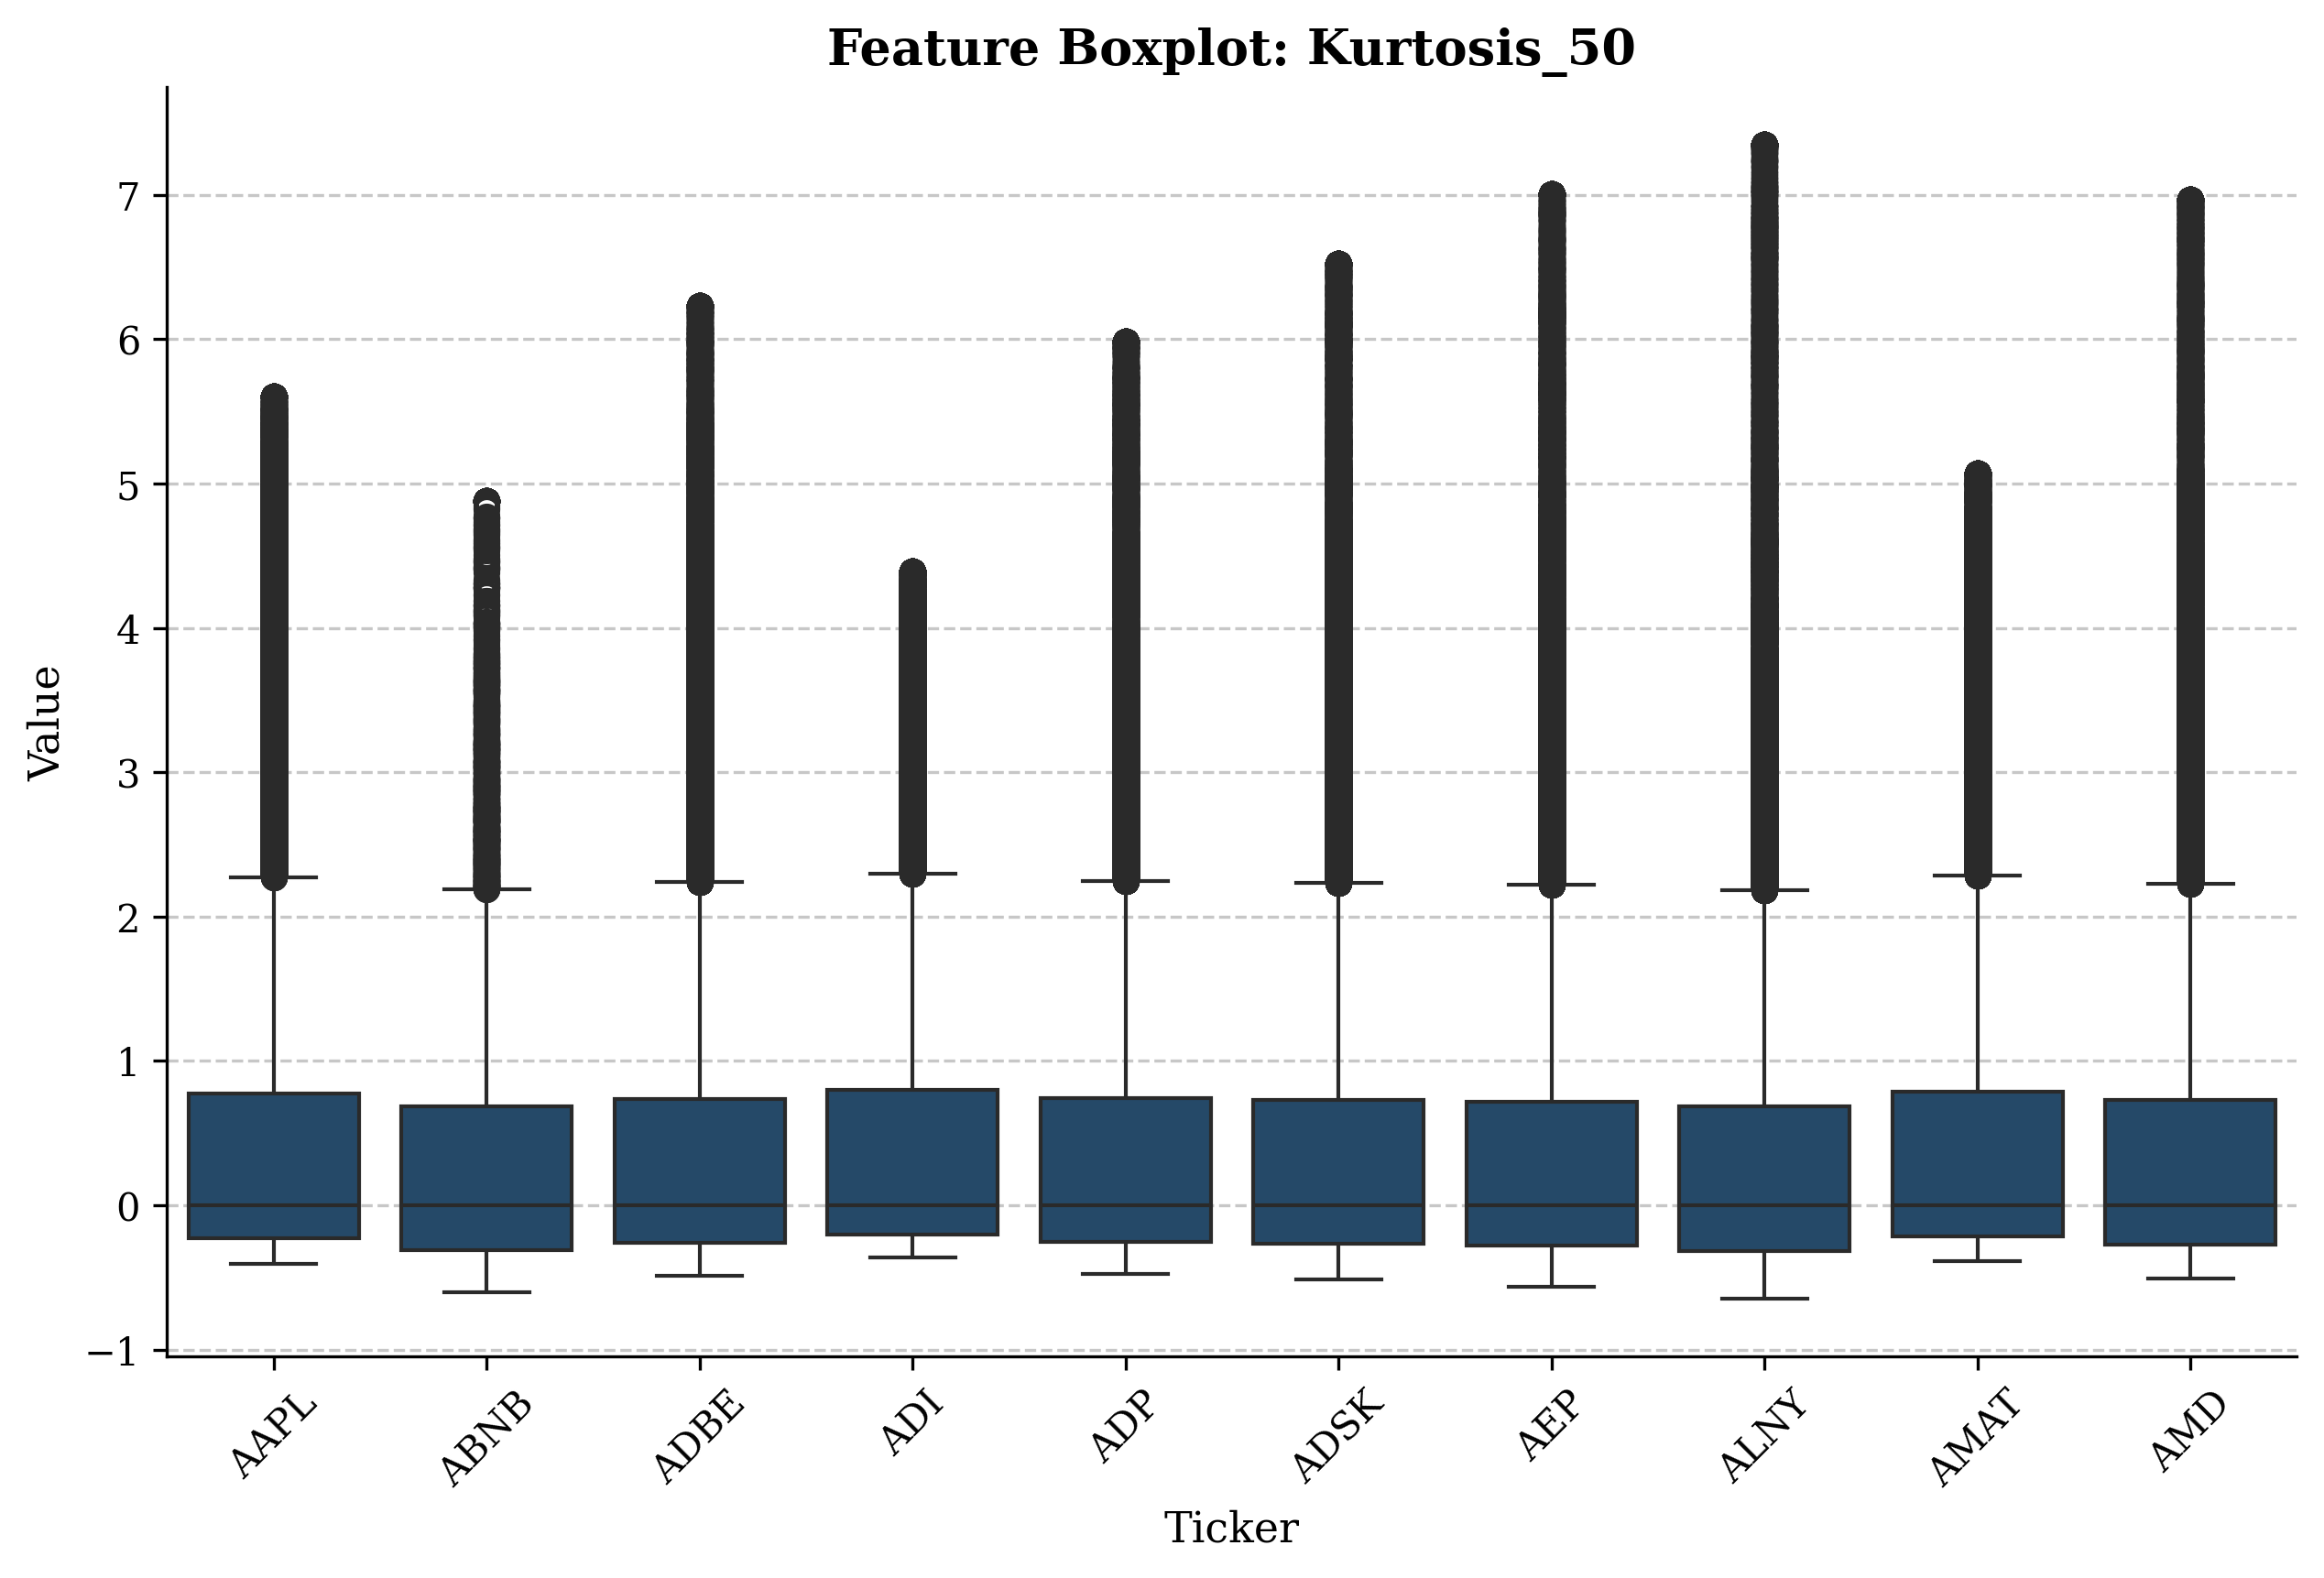
\includegraphics[width=\textwidth]{plots/boxplots/robustscaled_winsorized_1.0_percentiles/Kurtosis_50_boxplot.png}
        \caption{Boxplot for kurtosis}
        \label{fig:boxplot_robustscaled_winsorized_1.0_percentiles_Kurtosis_50}
    \end{subfigure}

    \caption{Boxplot of the data that was first winsorized and then scaled with the robust scaling method on selected tickers.}
    \label{fig:boxplot_robustscaled_winsorized_1.0_percentiles}
\end{figure}

\subsubsection{Range Clipping}
Despite robust scaling, individual features can still take on values outside the expected range due to extreme volatility. As the distribution diagram for the kurtosis feature (see Figure \ref{fig:boxplot_robustscaled_winsorized_1.0_percentiles_Kurtosis_50} shows, a final “hard clipping” is performed. This limits all features of each ticker $n$ to the interval $[-5, 5]$. The choice of this range is based on testing where the different models were most stable during training. 
% Activation functions such as Tanh or Sigmoid are sensitive to the input scaling. Values far outside of ±3 standard deviations can lead to vanishing or exploding gradients. The chosen range represents a heuristic compromise.
\subsubsection{Data Leakage}
To avoid data leakage, all parameters, the percentiles for winsorization and the median and \gls{iqr} for robust scaling were calculated based exclusively on the training set and then applied to the validation and testing sets. This ensures that no future information is leaked into the scaling logic of the training phase. 
\subsubsection{Handling Target Variables}
The target variables, the log-returns for the selected horizons, were only scaled, but not winsorized nor clipped. This approach aims to preserve actually price jumps or crashes, which the model should be able to predict. 


\section{Baselines}

\subsection{Overview of All features}

All the engineered features are categorized into three hierarchical complexity levels. A distinction must be made between a \textbf{base indicator}  and the resulting \textbf{input dimensions}, since many indicators depend on variable lookback horizons, a single base indicator can yield multiple input features. For instance, a Simple Moving Average (SMA) calculated using lookback periods of 20, 50, and 200, results in three distinct feature columns (input dimensions). 

To evaluate the predictive power of the complexity levels each combination is tested, resulting in seven different combinations overall. 
Table \ref{tab:feature_distribution} summarizes the distribution of base indicators and their corresponding total feature dimensions across the seven defined complexity permutations. 
A comprehensive list detailing each feature and its explanatory value can found in Appendix \ref{tab:appendix_features}. 

\begin{table}[htbp]
\centering
\caption{Overview of feature Ccmplexity permutations and dimensions}
\label{tab:feature_distribution}
\begin{tabular}{llcc}
\toprule
\textbf{Complexity Def.} & \textbf{Complexity Levels} & \textbf{ Base Indicators} & \textbf{Total Dimensions} \\
\midrule
$C_{L10}$ & 10 & 3 & 8 \\
$C_{L20}$ & 20 & 12 & 28 \\
$C_{L30}$ & 30 & 13 & 14 \\
\midrule
$C_{L10+L20}$ & 10 + 20 & 15 & 36 \\
$C_{L10+L30}$ & 10 + 30 & 16 & 22 \\
$C_{L20+L30}$ & 20 + 30 & 25 & 42 \\
$C_{L10+L20+L30}$ & 10 + 20 + 30 & 28 & 50 \\
\bottomrule
\end{tabular}
\end{table}


This approach allows for a detailed analysis of how different types of information contribute to the models forecasting accuracy. It also shows potential redundancies and synergies within the feature sets. 




\subsection{Models}

The following models were selected for this evaluation and were classified according to the proposed models properties. They cover a range from traditional statistical estimators to state-of-the-art deep learning architectures.

\subsubsection{Linear Regression}
As the simplest model for this evaluation, a linear regression model is chosen to serve a predictive baseline estimator. More specifically an \gls{ols} regression is implemented. It can model linear relationships between the input features and the target returns.

The primary advantage of this estimator is its computational efficiency and high interpretability. Its limitations are the lack of ability to capture non-linear relationships or temporal dependencies between the variables.
% For implementation the LinearRegression from scikit-learn was used.



\subsubsection{Random Forest}
The \gls{rf} recursivly splits the feature space, which allows it to model non-linear dependencies. The \gls{rf} is a non-parametric model, meaning its complexity is dependent on the training data distribution instead of a fixed set of weights. 

Although the \gls{rf} can capture complex relationships between features at a specific timestamp, it treats each observation as an independent instance. This results in the model ignoring the sequential order or temportal context in the time series.
    

\subsubsection{\gls{mlp}}
The \gls{mlp} represents the first model in this analysis incorporating deep learning. It can model non-linear dependencies with its activation functions, allowing it to build complex relationships within the input data. The structure of the network is set before the learning process and during it, only the weights are adjusted accordingly. 
Like the previous estimators, the model is also context unaware. A flattened vector at time $t$ is used for prediction also ignoring the temporal context in the sequence. 

\subsubsection{\gls{patchtst}}
Representing the current state-of-the-art in long-term time series forecasting, the Patch Time Series Transformer (\gls{patchtst}) was chosen \cite{nie2023timeseriesworth64}.

It utilizes two unique concepts compared to traditional Transformers, dividing the input data into patches and handling multivariate time series independently. 

\begin{itemize}
    \item \textbf{Patching:} Instead of embedding each individual data point, patches are used. A patch consists of a sequence of a set length, capturing multiple data points. This allows the model to capture local semantic information within each patch. 
    Patchwise embeddings instead of pointwise embeddings help to reduce the computational complexity from $O(L^2)$ to $O((L/S)^2)$, where $L$ is the sequence length and $S$ is the stride, the non-overlapping part of the input patch. 
    
    \item \textbf{Channel-Independence:} The model handles each feature channel as an univariate time series but they share the same weights in the encoder. This allows the model to learn temporal pattern across channels without beeing corrupted by the high dimensionality of the original multivariate signal. 

\end{itemize}

\gls{patchtst} utilizes only the encoder part of the traditional Transformers, in which each embedding is transformed into an abstract representation. These representations are then used in a regression head, which in this case is for forecasting the different time horizons. 

The self-attention mechanism allows the estimator to learn dependencies across different timesteps within the lookback window.
% The model was implemented with the help of the library transformers from huggingface. 



\subsection{Model Categorization Matrix}
The Table \ref{tab:ModelCategorizationMatrix} displays the classification of each model.

\begin{table}[htbp]
\centering
\caption{Classification of selected models}
\label{tab:ModelCategorizationMatrix}
\begin{tabular}{llll}
\toprule
\textbf{Model} & \textbf{Linearity} & \textbf{Parametric} & \textbf{Temporal Awareness} \\ 
\midrule
Linear Regression             & Linear             & Yes                 & No (Pointwise)             \\
Random Forest                 & Non-Linear         & No                  & No (Pointwise)             \\
\gls{mlp}                     & Non-Linear         & Yes                 & No (Pointwise)             \\
PatchTST                      & Non-Linear         & Yes                 & Yes (Context-aware)        \\ 
\bottomrule
\end{tabular}
\end{table}

\subsection{Complexity Hierarchy Justification}

\begin{enumerate}
\item \textbf{Level 1: Linear Regression:} Assumes global linearity and serves as the baseline.
\item \textbf{Level 2: Random Forest:} Introduces non-linear decision boundaries through recursive data splits.
\item \textbf{Level 3: \gls{mlp}:} Utilizes hidden layers to learn abstract feature representations.
\item \textbf{Level 4: \gls{patchtst}:} Integrates deep neural layers with a multi-head attention mechanism to capture sequential structure and long-range dependencies in the data.
\end{enumerate}

\section{Experimental Setup}
Following the methodology described in Section \ref{ch:overview}, the parameters are specified. After the preprocessing step, which resulted in the removal of nine tickers, the dataset consists of $n \in \{1, 2, \dots, 92\}$ individual tickers. The chosen horizons for this study are $H = \{6, 12, 24, 48\}$, which corresponds to forecasting horizons of 30, 60, 120 and 240 minutes respectively. Therefore, the models prediction vector for each time step $t$ and ticker $n$ results in the dimension $\hat{\mathbf{y}}_{t, n} \in \mathbb{R}^4$.



\section{Metrics}
To provide a robust method for model evaluation, two sets of metrics are used. 
First, statistical methods to evaluate the point forecast  accuracy of the models. Second, economic metrics are utilized to evaluate the models performance with a simulated trading strategy.

\subsection{Statistical Metrics}
    These metrics evaluate the error between the predicted returns and the actual ground-truth values. 

    \paragraph{Mean Sqared Error:} The \gls{mse} penalizes large outliers quadratically. 
    \begin{equation}
        MSE = \frac{1}{n} \sum_{i=1}^{n} (y_i - \hat{y}_i)^2
    \end{equation}

    \paragraph{Mean Absolute Error:} The \gls{mae} is a more robust measure against outliers because differences are not squared.
    \begin{equation}
        MAE = \frac{1}{n} \sum_{i=1}^{n} |y_i - \hat{y}_i|
    \end{equation}

        % \paragraph{\gls{r2}}:  determines how good the model estimates the variance of the dependent variable. 
        % calculatioan: 
        % In financial time series a low \gls{r2} is already very good. This is because markets are highly efficient and the signal to noise ratio of data is really low random walk. \cite{Gu2020AssetPricing}

\subsection{Economic Evaluation - Mean-Variance Analysis}
To evaluate the economic performance, a \gls{mvo} is performed. This framework assesses the profitability of the model as a systematic investment strategy, providing a practical perspective in contrast to the statistical metrics.
At every $m$-th timestep $t$, where $m = h \in H$ 
an optimal portfolio is constructed. This process takes two primary inputs: expected returns and a risk model.

\paragraph{Expected Returns:} The models point predictions are used as the estimates for future returns. These are annualized based on the specific horizon $h$.
\paragraph{Risk Model:} The covariance matrix is calculated using historical returns from the training set to avoid look-ahead bias. For this step, Ledoit-Wolf shrinkage is utilized to ensure a stable covariance matrix.

The ground-truth returns of the tickers are multiplied by the resulting weight vector of the optimal portfolio to determine the performance. 
This procedure is applied across the entire test set, over all horizons $H$, resulting in the annualized return and the annualized Sharpe ratio 
for each of the four horizons respectively. While portfolio rebalancing costs are not considered, the results still provide a risk-adjusted view of the models. 
The annualized return represents the total return the strategy would yield over a one-year period. The annualized Sharpe ratio measures the risk-adjusted performance. It indicates how much return is generated per unit of risk, which is defined as the standard deviation of the returns.

\section{Training Process with Hyperparameter Tuning}
The models hyperparameters are selected through a hyperparameter tuning process. Due to the high computational demand of training all configurations across every complexity level $C_k$, the process was restricted to a subset of $N = 5$ tickers.

The training process is performed using a specific subset of the available hyperparameter configurations. After the training phase, each configuration is evaluated by generating predictions on the validation dataset. The evaluation is performed between the predicted values $\hat{\mathbf{y}}_{t, n}$ of the model and the ground-truth values $\mathbf{y}_{t, n}$ using the loss function \gls{mae}. 

This process is performed for $10$ iterations, where each configuration is randomly sampled from the available hyperparameter space. After the hyperparameter tuning process has finished, the configuration with the lowest validation loss is selected for the final model training on the combined training and validation sets.

The training was conducted on a workstation with an AMD Ryzen 7 3800X as CPU and a Nvidia 2060 Super as GPU.



\subsection{Final Model Parameters}

\paragraph{Linear Regression:}
The chosen baseline is an \gls{ols} linear regression, which was utilized without hyperparameter training.

\paragraph{\gls{rf}:}
The search grid for the \gls{rf} hyperparameters and the final selected parameters are presented in Appendix \ref{app:rf_params}. For computational reasons due to the large dataset, the \gls{mse} was utilized as the split criterion instead of the \gls{mae}.

\paragraph{\gls{mlp}:}
The architecture of the \gls{mlp} was selected based on the parameter space provided in Appendix \ref{app:mlp_params}. It also represents the final configuration used for evaluation.

\paragraph{\gls{patchtst}:}
For the Transformer \gls{patchtst}, the parameter space and the resulting optimal parameters are shown in Appendix \ref{app:patchtst_params}.





\section{Quantitative Analysis}
The model evaluation is based on both statistical metrics and economic performance. To assess whether the increasing levels of feature complexity $C_k$ provide any predictive value, a "Constant Model" is introduced as a baseline.
This baseline predicts a constant value for all timesteps in the training set and is optimized to minimize the \gls{mae} \textbf{without utilizing any} input features, for each horizon $h$ respectively.
Because of the mathematical properties of the \gls{mae}, the optimal constant predictor corresponds to the median of the target distribution. This model serves as a benchmark to determine if the more sophisticated models actually benefit from the different complexity levels or if a simple statistical average would yield similar results in the context of this study.

\subsection{Machine Learning Performance Metrics}
Evaluating all models on the test dataset in Table \ref{tab:model_eval}, it can be observed that all machine learning models perform relatively similar. However, nearly all of them either cannot outperform or perform only equally to the Constant Model.
Complex models like \gls{patchtst} did not show any advantage over simpler models.

Furthermore, a more complex feature set, which resulted in an increasing dimension of the dataset, did not help to increase the signal-to-noise ratio. The fact that even the more complex models could not benefit from the computed features underlines the difficulties in this forecasting task.

\subsection{Economic Evaluation Metrics}
For the models economic evaluation, a mean-variance analysis was performed. The corresponding metrics are presented in Table \ref{tab:economic_eval}.

Although relatively high return values can be observed, a comparison with the Constant Model reveals that these results are not caused by superior model performance, but by the models performing similar to the baseline. The strong performance of the Constant Model is primarily driven by a slightly positive median in the training distribution. As this upward trend continued throughout the testing period, the model effectively captured the market's positive drift, resulting in long-term profits without the need for any predictive features. 
Furthermore, these results do not account for transaction costs, which would significantly affect the outcome, especially for shorter horizons. For the horizon $h = 6$, the portfolio was rebalanced 2,929 times, whereas for the horizon $h = 48$, it was rebalanced 367 times over the testing period. These high turnover rates would add substantial transaction costs in an actual trading strategy.


\begin{landscape}
\captionof{table}{The \gls{mae} and \gls{mse} were computed on the unscaled predicted returns. The numbers are scaled to better visualize the results.}
\label{tab:model_eval}
\begin{tabular}{p{2.2cm} p{1.5cm}|*{10}{>{\centering\arraybackslash}p{1.1cm}}}
\toprule
 &  & \multicolumn{2}{c}{Constant Model} & \multicolumn{2}{c}{Linear Regression} & \multicolumn{2}{c}{Random Forest} & \multicolumn{2}{c}{MLP} & \multicolumn{2}{c}{PatchTST} \\
 &  & MSE ($10^{-6}$) & MAE ($10^{-4}$) & MSE ($10^{-6}$) & MAE ($10^{-4}$) & MSE ($10^{-6}$) & MAE ($10^{-4}$) & MSE ($10^{-6}$) & MAE ($10^{-4}$) & MSE ($10^{-6}$) & MAE ($10^{-4}$) \\
Complexity & Horizon &  &  &  &  &  &  &  &  &  &  \\
\midrule 
\multirow[t]{4}{*}{$C_{L10}$} & 6 & 16.82 & 27.75 & 16.84 & 27.78 & 16.89 & 27.86 & 16.82 & 27.75 & 16.83 & 27.75 \\
 & 12 & 35.30 & 40.89 & 35.36 & 40.95 & 35.63 & 41.19 & 35.31 & 40.90 & 35.35 & 40.93 \\
 & 24 & 74.96 & 61.18 & 75.18 & 61.29 & 76.26 & 62.08 & 74.99 & 61.18 & 75.07 & 61.22 \\
 & 48 & 156.57 & 90.95 & 157.36 & 91.22 & 161.26 & 93.39 & 156.74 & 90.98 & 157.06 & 91.04 \\
\cline{1-12}
\multirow[t]{4}{*}{$C_{L20}$} & 6 & 16.82 & 27.75 & 16.89 & 27.87 & 16.92 & 27.83 & 16.83 & 27.77 & 16.88 & 27.86 \\
 & 12 & 35.30 & 40.89 & 35.56 & 41.17 & 35.71 & 41.13 & 35.37 & 40.94 & 35.53 & 41.11 \\
 & 24 & 74.96 & 61.18 & 75.77 & 61.85 & 75.84 & 61.66 & 75.34 & 61.40 & 75.69 & 61.54 \\
 & 48 & 156.57 & 90.95 & 159.11 & 92.28 & 158.35 & 91.78 & 157.53 & 91.36 & 158.47 & 91.63 \\
\cline{1-12}
\multirow[t]{4}{*}{$C_{L30}$} & 6 & 16.82 & 27.75 & 16.84 & 27.78 & 16.90 & 27.85 & 16.83 & 27.77 & 16.87 & 27.84 \\
 & 12 & 35.30 & 40.89 & 35.38 & 40.97 & 35.65 & 41.14 & 35.34 & 40.94 & 35.39 & 40.96 \\
 & 24 & 74.96 & 61.18 & 75.13 & 61.31 & 75.64 & 61.55 & 74.99 & 61.20 & 75.32 & 61.33 \\
 & 48 & 156.57 & 90.95 & 156.81 & 91.11 & 157.40 & 91.32 & 156.42 & 90.88 & 157.96 & 91.42 \\
\cline{1-12}
\multirow[t]{4}{*}{$C_{L10+L20}$} & 6 & 16.82 & 27.75 & 16.91 & 27.88 & 16.91 & 27.87 & 16.84 & 27.77 & 16.85 & 27.79 \\     
 & 12 & 35.30 & 40.89 & 35.59 & 41.19 & 35.73 & 41.25 & 35.37 & 40.94 & 35.45 & 41.05 \\
 & 24 & 74.96 & 61.18 & 76.01 & 61.94 & 76.08 & 61.93 & 75.17 & 61.27 & 75.43 & 61.52 \\
 & 48 & 156.57 & 90.95 & 159.75 & 92.34 & 159.23 & 92.41 & 157.06 & 91.14 & 158.94 & 91.70 \\
\cline{1-12}
\multirow[t]{4}{*}{$C_{L10+L30}$} & 6 & 16.82 & 27.75 & 16.87 & 27.81 & 16.92 & 27.87 & 16.85 & 27.79 & 16.84 & 27.75 \\     
 & 12 & 35.30 & 40.89 & 35.49 & 41.04 & 35.74 & 41.26 & 35.38 & 40.94 & 35.36 & 40.91 \\
 & 24 & 74.96 & 61.18 & 75.50 & 61.48 & 76.16 & 62.00 & 75.09 & 61.21 & 75.03 & 61.17 \\
 & 48 & 156.57 & 90.95 & 157.86 & 91.43 & 159.06 & 92.41 & 156.75 & 91.02 & 157.40 & 91.26 \\
\cline{1-12}
\multirow[t]{4}{*}{$C_{L20+L30}$} & 6 & 16.82 & 27.75 & 16.89 & 27.85 & 16.92 & 27.83 & 16.83 & 27.76 & 16.88 & 27.80 \\     
 & 12 & 35.30 & 40.89 & 35.58 & 41.17 & 35.70 & 41.13 & 35.30 & 40.90 & 35.48 & 41.02 \\
 & 24 & 74.96 & 61.18 & 75.96 & 61.92 & 75.78 & 61.61 & 74.96 & 61.17 & 75.40 & 61.34 \\
 & 48 & 156.57 & 90.95 & 159.70 & 92.45 & 158.12 & 91.67 & 156.57 & 90.94 & 158.37 & 91.54 \\
\cline{1-12}
\multirow[t]{4}{*}{$C_{L10+L20+L30}$} & 6 & 16.82 & 27.75 & 16.91 & 27.88 & 16.93 & 27.86 & 16.82 & 27.75 & 16.91 & 27.86 \\ 
 & 12 & 35.30 & 40.89 & 35.63 & 41.22 & 35.75 & 41.23 & 35.30 & 40.90 & 35.47 & 41.01 \\
 & 24 & 74.96 & 61.18 & 76.17 & 62.02 & 76.00 & 61.83 & 74.96 & 61.18 & 75.56 & 61.43 \\
 & 48 & 156.57 & 90.95 & 160.18 & 92.47 & 158.80 & 92.13 & 156.57 & 90.95 & 159.05 & 91.74 \\
\cline{1-12}
\bottomrule
\end{tabular}

\captionof{table}{The "Return" represents the annualized return and "Sharpe" the Sharpe ratio over the testing period repecitvely.}
%\resizebox{\textwidth}{!}{
\label{tab:economic_eval}
\begin{tabular}{p{2.2cm} p{1.5cm}|*{10}{>{\centering\arraybackslash}p{1.1cm}}}
\toprule
 &  & \multicolumn{2}{c}{Constant Model} & \multicolumn{2}{c}{Linear Regression} & \multicolumn{2}{c}{Random Forest} & \multicolumn{2}{c}{MLP} & \multicolumn{2}{c}{PatchTST} \\
 &  & Return (\%) & Sharpe & Return (\%) & Sharpe & Return (\%) & Sharpe & Return (\%) & Sharpe & Return (\%) & Sharpe \\
Complexity & Horizon &  &  &  &  &  &  &  &  &  &  \\
\midrule
\multirow[t]{4}{*}{$C_{L10}$} & 6 & 53.11 & 2.03 & 25.71 & 1.09 & 39.78 & 1.62 & 62.11 & 2.56 & 33.58 & 1.55 \\
 & 12 & 58.45 & 2.15 & 40.35 & 1.77 & 33.45 & 1.27 & 57.12 & 2.21 & 40.37 & 1.81 \\
 & 24 & 53.94 & 1.91 & 40.92 & 1.81 & 48.59 & 1.79 & 51.32 & 1.91 & 42.55 & 1.76 \\
 & 48 & 51.42 & 1.77 & 38.43 & 1.73 & 54.55 & 1.97 & 49.07 & 1.81 & 43.81 & 1.79 \\
\cline{1-12}
\multirow[t]{4}{*}{$C_{L20}$} & 6 & 53.11 & 2.03 & 39.10 & 1.69 & 32.73 & 1.42 & 51.37 & 2.13 & 52.58 & 2.40 \\
 & 12 & 58.45 & 2.15 & 40.84 & 1.70 & 32.18 & 1.34 & 61.96 & 2.58 & 45.54 & 2.04 \\
 & 24 & 53.94 & 1.91 & 52.05 & 2.14 & 35.67 & 1.50 & 55.17 & 2.29 & 28.10 & 1.17 \\
 & 48 & 51.42 & 1.77 & 49.97 & 2.03 & 58.68 & 2.30 & 43.73 & 1.79 & 22.76 & 0.86 \\
\cline{1-12}
\multirow[t]{4}{*}{$C_{L30}$} & 6 & 53.11 & 2.03 & 50.05 & 2.14 & 1.22 & 0.05 & 59.07 & 2.45 & 36.47 & 1.66 \\
 & 12 & 58.45 & 2.15 & 45.00 & 1.86 & -0.16 & -0.01 & 57.28 & 2.24 & 41.07 & 1.74 \\
 & 24 & 53.94 & 1.91 & 49.82 & 2.04 & -0.53 & -0.02 & 47.06 & 1.79 & 53.45 & 2.22 \\
 & 48 & 51.42 & 1.77 & 44.71 & 1.60 & 30.85 & 1.15 & 46.60 & 1.68 & 33.33 & 1.39 \\
\cline{1-12}
\multirow[t]{4}{*}{$C_{L10+L20}$} & 6 & 53.11 & 2.03 & 44.64 & 1.99 & 44.09 & 1.88 & 59.19 & 2.68 & 42.29 & 1.86 \\
 & 12 & 58.45 & 2.15 & 41.84 & 1.84 & 40.13 & 1.66 & 67.91 & 2.89 & 49.00 & 2.16 \\
 & 24 & 53.94 & 1.91 & 44.10 & 1.96 & 54.45 & 2.19 & 61.25 & 2.62 & 49.00 & 2.09 \\
 & 48 & 51.42 & 1.77 & 35.40 & 1.63 & 63.60 & 2.45 & 54.99 & 2.28 & 41.69 & 1.80 \\
\cline{1-12}
\multirow[t]{4}{*}{$C_{L10+L30}$} & 6 & 53.11 & 2.03 & 35.44 & 1.55 & 35.27 & 1.45 & 57.12 & 2.39 & 45.10 & 2.07 \\
 & 12 & 58.45 & 2.15 & 41.98 & 1.90 & 14.26 & 0.55 & 48.47 & 1.97 & 46.68 & 2.04 \\
 & 24 & 53.94 & 1.91 & 39.96 & 1.75 & 25.54 & 0.97 & 40.87 & 1.56 & 43.37 & 1.74 \\
 & 48 & 51.42 & 1.77 & 34.37 & 1.52 & 21.86 & 0.78 & 37.73 & 1.33 & 37.01 & 1.59 \\
\cline{1-12}
\multirow[t]{4}{*}{$C_{L20+L30}$} & 6 & 53.11 & 2.03 & 51.69 & 2.23 & 21.04 & 0.91 & 53.20 & 2.04 & 41.00 & 1.81 \\
 & 12 & 58.45 & 2.15 & 52.34 & 2.19 & 8.86 & 0.37 & 58.63 & 2.15 & 26.02 & 1.08 \\
 & 24 & 53.94 & 1.91 & 56.43 & 2.40 & 29.76 & 1.23 & 53.78 & 1.94 & 33.15 & 1.29 \\
 & 48 & 51.42 & 1.77 & 43.27 & 1.84 & 31.34 & 1.20 & 51.03 & 1.76 & 42.70 & 1.67 \\
\cline{1-12}
\multirow[t]{4}{*}{$C_{L10+L20+L30}$} & 6 & 53.11 & 2.03 & 47.28 & 2.11 & 29.76 & 1.26 & 53.11 & 2.03 & 50.36 & 2.37 \\      
 & 12 & 58.45 & 2.15 & 50.32 & 2.21 & 33.24 & 1.34 & 58.45 & 2.15 & 60.90 & 2.60 \\
 & 24 & 53.94 & 1.91 & 38.05 & 1.73 & 43.59 & 1.77 & 54.39 & 1.91 & 51.61 & 2.21 \\
 & 48 & 51.42 & 1.77 & 42.69 & 1.96 & 47.66 & 1.80 & 51.88 & 1.77 & 47.96 & 2.04 \\
\cline{1-12}
\bottomrule
\end{tabular}
%}

\end{landscape}

\section{Qualitative Analysis}

% Show here plots about prediction/ trainings plots 
To understand the discrepancy between complex models and their limited predictive power, this section examines the underlying possible causes. 
The analysis focuses on four key areas:  
\begin{itemize}
    \item Dataset shifts
    \item Training dynamics
    \item Model predictions
    \item Impact of feature complexity and \gls{emh}
\end{itemize}

\subsubsection{Dataset Discrepancy and Non-Stationarity}
A primary challenge in financial forecasting is the non-stationarity of the data. Comparing the two main features (volume and return), from which most other features are calculated on, across the training, validation and testing sets reveals a distribution shift (see Table \ref{tab:dataset_discrepancy}).


\begin{table}[htbp]
\centering
\caption{Descriptive statistics of scaled features (with robust scaling method) across datasets for AAPL, similar shifts can be observed for other tickers.}
\label{tab:dataset_discrepancy}
\begin{tabular}{@{}llccc@{}}
\toprule
\textbf{Feature} & \textbf{Dataset} & \textbf{Mean} & \textbf{Std} & \textbf{Median} \\ \midrule
\multirow{3}{*}{LOGRET\_1} & Training & 0.01 & 1.09 & 0.00 \\
 & Validation & 0.01 & 1.34 & 0.00 \\
 & Test & 0.01 & 0.91 & 0.02 \\ \midrule
\multirow{3}{*}{LOG\_VOLUME} & Training & 0.05 & 0.73 & -0.00 \\
 & Validation & -0.39 & 0.57 & -0.45 \\
 & Test & -0.78 & 0.55 & -0.87 \\ \bottomrule
\end{tabular}
\end{table}

The discrepancy in performance can be partly explained by the shift in the log-volume feature. The median shifts from $0.00$ in the training set to $-0.87$ in the test set. This suggests that the market environment during the testing period differed fundamentally from the training phase. Additionally, the standard deviation of 5-minute log-returns (LOGRET\_1) increases from $1.09$ to $1.34$ between training and validation. In finance, this increase in volatility represents a shift in risk regimes. Such non-stationary behavior can explain why patterns learned during training fail to generalize to the validation set.


\subsubsection{Training Dynamics and Overfitting}

To further examine the model quality, the learning curves of the deep learning models (trained without early stopping) are presented in Figure \ref{fig:learning curves}.

For the deep learning architectures (\gls{mlp} and \gls{patchtst}), a rapid divergence between training and validation loss is observed. While the models are capable of reducing the training loss nearly to zero, the validation error remains stagnant or increases slightly. This indicates a lack of a learnable, generalizable signal.

\begin{figure}[htbp]
\centering
\begin{subfigure}[b]{0.49\textwidth}
\centering
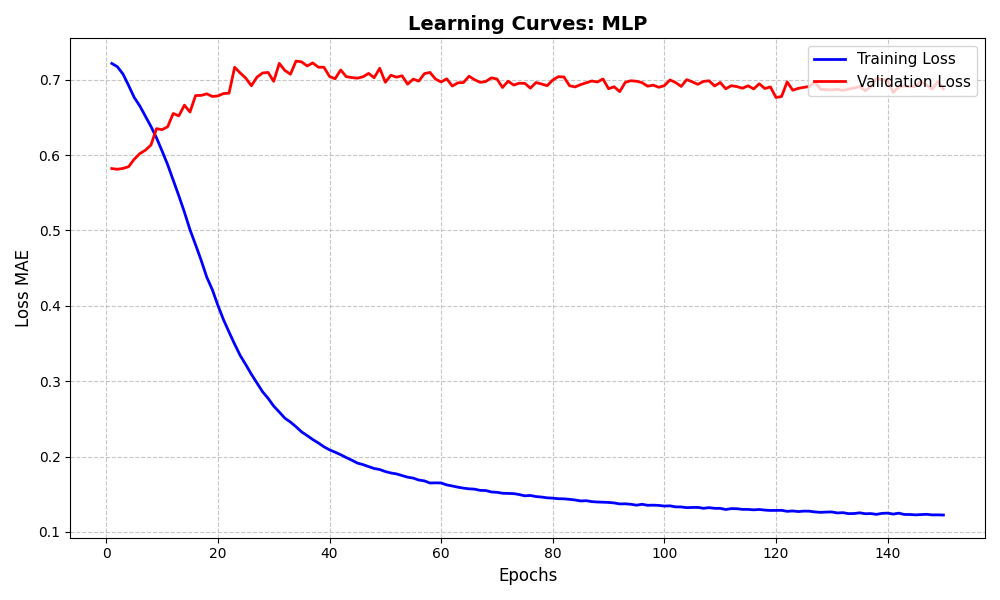
\includegraphics[width=\textwidth]{plots/learning_curves/MLP_learning_curve.png}
\caption{Learning curve for \gls{mlp}}
\label{fig:learning_curve_mlp}
\end{subfigure}
\hfill
\begin{subfigure}[b]{0.49\textwidth}
\centering
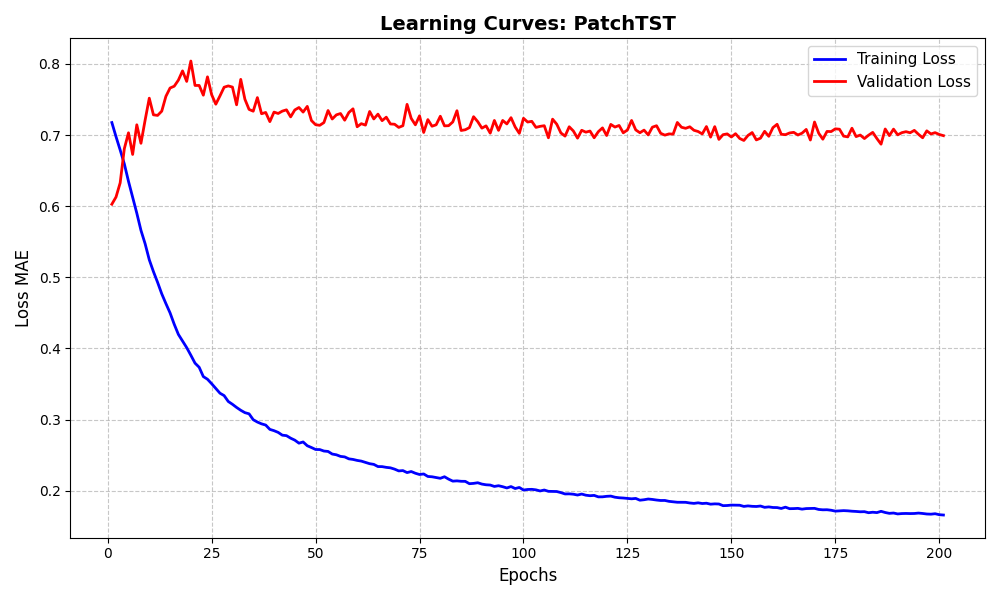
\includegraphics[width=\textwidth]{plots/learning_curves/PatchTST_learning_curve.png}
\caption{Learning curve for \gls{patchtst}}
\label{fig:learning_curve_patchtst}
\end{subfigure}
\caption[Learning Curves]{Training Curves}
\label{fig:learning curves}
\end{figure}


\subsubsection{Predictabilty of Models}
To gain a clearer understanding, the model predictions for \gls{patchtst} is visualized against the ground truth (see Figure \ref{fig:predictions_patchtst}). A key observation is that all models exhibit a significantly lower standard deviation in their predictions compared to the actual target variables (summarized in Table \ref{tab:prediction_stats}).

\begin{table}[htbp]
\centering
\caption{Comparison of statistical properties: Ground truth vs. model predictions of all models (Horizon $h=6$ and complexity $C_k = C_{L10+L20+L30}$)}
\label{tab:prediction_stats}
\begin{tabular}{lccc}
\toprule
\textbf{Model} & \textbf{Mean ($10^{-4}$)} & \textbf{Median ($10^{-4}$)} & \textbf{Vol. ($\sigma$) ($10^{-4}$)} \\ \midrule
\textbf{Ground Truth ($y$)} & \textbf{1.0086} & \textbf{1.4515} & \textbf{41.0195} \\ \midrule
Constant Model     & 0.8631 & 0.8631 & 0.0000 \\
Linear Regression  & 0.4108 & 0.2734 & 2.9257 \\
Random Forest      & -0.0478 & -0.0575 & 2.9138 \\
MLP                & 0.7690 & 0.5573 & 0.3127 \\
PatchTST           & 0.4323 & 0.5644 & 2.7786 \\
\bottomrule
\end{tabular}
\end{table}

Mathematically, this behavior is a consequence of the chosen loss functions. When a model minimizes the \gls{mse} in an environment with a low signal-to-noise ratio, the optimal strategy, without any learnable patterns, is to predict the expected value:

$$\hat{y} = E[y | x] \approx \bar{y}$$

Financial time series exhibit a low signal-to-noise ratio. If the data does not represent enough predictive information, the model attempts to use the average to minimize the effect of outliers. The model defaults to the "safest" statistical estimate, the mean of the distribution, which is approximately zero. For models optimized via \gls{mae}, the equivalent "safe" strategy is predicting the median. Since log-returns are approximately symmetrically distributed around zero (median $\approx$ mean $\approx 0$), both strategies result in mean-like predictions that fail to capture profitable price movements.


\begin{figure}[htbp]
\centering
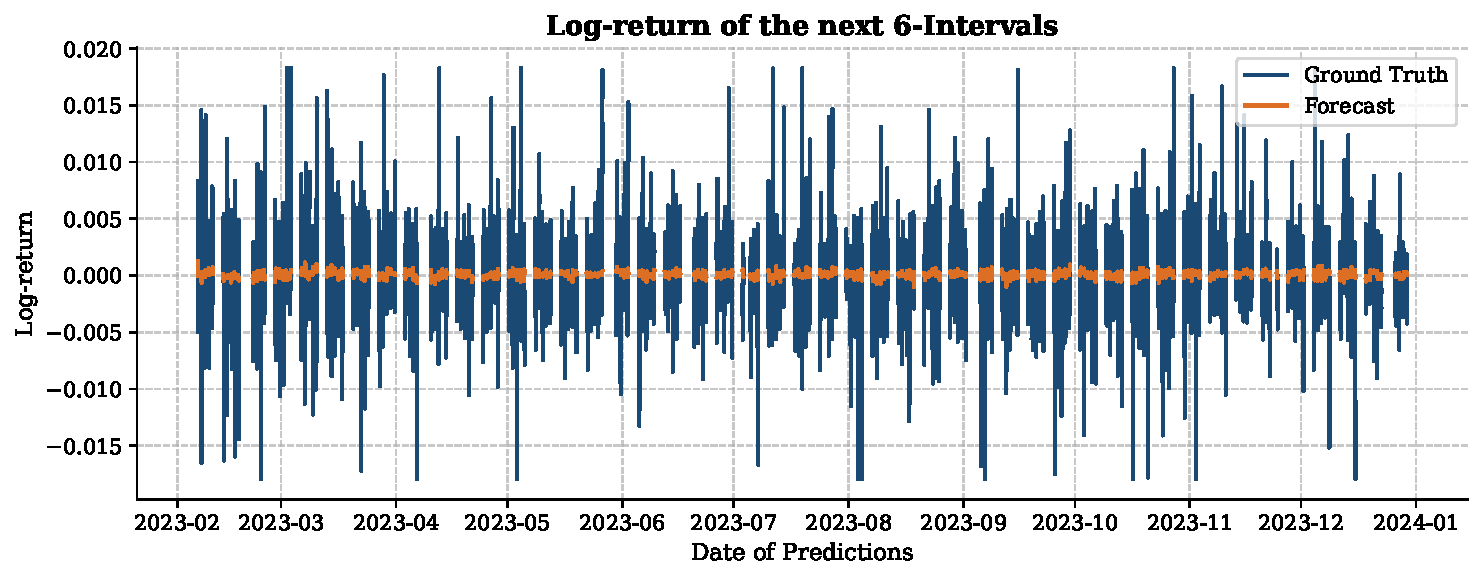
\includegraphics[width=\textwidth]{plots/predictions/weekly_predictions_target_6.pdf}
\caption{Comparison of predicted log-returns compared to ground truth for \gls{patchtst} (Horizon $h=6$ and complexity $C_k = C_{L10+L20+L30}$).
}
\label{fig:predictions_patchtst}
\end{figure}


\subsubsection{Feature Complexity and Market Efficiency}

The introduction of increasingly complex features ($C_{L10}$ to $C_{L10+L20+L30}$) did not lead to a measurable impact on performance. This suggests that the "Microstructure Noise" at the 5-minute resolution exhibits the true signal. These findings align with the \gls{emh}, suggesting that at this frequency, price movements closely follow a random walk. This, makes it nearly impossible for models to extract generalizable patterns besides learning the long term trend using only historical \gls{ohlcv} data.


\chapter{Conclusion}
\label{ch:conclusion}


\section{Summary of Findings}

This study demonstrates that predicting the short-term returns of individual tickers remains a very challenging task. It shows that models ranging from simple linear regression to state-of-the-art Transformers like \gls{patchtst} struggle to extract predictive information from technical indicators at a 5-minute resolution.

Instead of learning generalizable market dynamics, complex models exhibited immediate overfitting, while simpler models defaulted to a mean-prediction strategy. These results suggest that at high frequencies, the signal-to-noise ratio is too low for standard supervised learning on price data alone.

\section{Future Research}

This study focused on high-frequency intraday data but it is noteworthy that literature on daily returns often shows more promising results, as microstructure noise is less present \cite{Kim2025Survey}.

Future research could expand upon these findings in several directions:

\begin{itemize}
\item \textbf{Alternative Data:} Including sentiment analysis or news feeds to provide non-price information.
\item \textbf{Order Book Depth:} Using Limit Order Book (LOB) data instead of just \gls{ohlcv} data to capture liquidity patterns.
\item \textbf{Alternative Loss Functions:} Exploring "Directional Accuracy" loss functions instead of \gls{mse}/\gls{mae}.
\end{itemize}

\newpage



\backmatter


%%%%%%%%%%%%%%%%%%%
%% create appendix
%%%%%%%%%%%%%%%%%%%



\appendix
\addchap{Appendix}

\addsec{Appendix A: Detailed Feature Specification}
\label{appendix:feature_specs}

 % load feature description csv - uncomment below
\begin{landscape}
\centering
\small
\csvreader[
    respect all,
    separator=semicolon,
    column count=6,
    longtable={p{0.18\linewidth} p{0.08\linewidth} p{0.18\linewidth} p{0.50\linewidth}},
    table head=
        \caption{Overview of all features used in this thesis, categorized by complexity level. Feature names are listed exactly as they appear in \texttt{feature\_config.json}. Indicator parameters can be retrieved from \texttt{feature\_config.json}, and implementation details can be found in \texttt{technical\_indicator.py}.}
        \label{tab:appendix_features}\\
        \toprule
        \textbf{Name} & \textbf{Cplx. Level} & \textbf{Category} & \textbf{Description} \\ \midrule
        \endfirsthead
        \multicolumn{4}{c}{{\bfseries \tablename\ \thetable{} -- continued from previous page}} \\
        \toprule
        \textbf{Name} & \textbf{Cplx.Level} & \textbf{Category} & \textbf{Description} \\ \midrule
        \endhead,
    table foot=\bottomrule,
    late after line=\\ \midrule,
    late after last line=\\
]{tables/thesis_feature_config_categorized.csv}
{
    1=\iname, 2=\icplx, 3=\icat, 4=\idesc
}
{
    \texttt{\iname} & \icplx & \icat & \idesc
}
\end{landscape}


\addsec{Appendix B: Setup Configuration (config.json)}
\label{app:config_json}
\begin{lstlisting}[language=json, caption={Example configuration file for the pipeline setup.}]
{
    "data": {
        "concatenated_csv": "data/concatenated/",
        "number_of_tickers": 3,
        "start_date": "2015-01-01",
        "end_date": "2023-12-31",
        "use_cached_processed_data": false,
        "processed_csv": "data/processed/"
    },
    "model": {
        "modelType": "MLP"
    },
    "features": {
        "featureConfigPath": "financial_TSF/features/feature_config.json",
        "complexity_levels": [
            10,
            20,
            30
        ]
    },
    "pipeline": {
        "steps": [
            "DataLoadingStep",
            "FeatureStep",
            "SplittingStep",
            "NormalizingStep",
            "TrainingStep",
            "EvaluationStep",
            "SavingStep"
        ]
    },
    "results": {
        "resultsPath": "results/"
    },
    "settings": {
        "forecast_horizon": [
            48
        ]
    }
}
\end{lstlisting}

\addsec{Appendix C: Pipeline Class}
\label{code:class_Pipeline}
\begin{lstlisting}[language=Python, caption={Implementation of pipeline class.}]
class Pipeline:
    def __init__(self, config_path: str = "financial_TSF/config.json"):
        with open(config_path, "r") as f:
            self.config: AppConfig = AppConfig.from_dict(json.load(f))
        self.model = MODEL_REGISTRY[self.config.model.model_type](self.config)
        self.steps: list[PipelineStep] = [
            STEP_REGISTRY[step_name](self.config) for step_name in self.config.pipeline.steps]
        
    def run(self, step_result: StepResult):
        step_result.model_instance = self.model
        for step in self.steps:
            print("--------------------------------------------------")
            print(f"Executing step: {step.__class__.__name__}")
            step_result = step.execute(step_result)
        return step_result
\end{lstlisting}



\addsec{Appendix D: Base Model Interface}
\label{code:class_BaseModel}
\begin{lstlisting}[language=Python, caption={Abstract base class for all model implementations.}]
class BaseModel(ABC):
    
    @abstractmethod
    def fit(self, step_result: StepResult) -> Any:
        pass
    @abstractmethod
    def predict(self, step_result: StepResult) -> tuple:
        pass
        
    def tune_hyperparameters(self, step_result: StepResult) -> dict | None:
        pass
\end{lstlisting}

\addsec{Appendix E: Base Model Interface}
\label{code:class_PipelineStep}
\begin{lstlisting}[language=Python, caption={Abstract base class for each pipeline step.}]
class PipelineStep(ABC):
    @abstractmethod
    def execute(self, step_result: StepResult) -> Any:
        pass
\end{lstlisting}

\addsec{Appendix F: Feature Configuration (feature\_config.json)}
\label{app:feature_config_json}
\begin{lstlisting}[language=json, caption={Feature Configuration - shortened for readability - complete file listed in code repository.}]
{
  "technical_indicators": {
    "SMA": {
      "enabled": true,
      "params": [
        20,
        50,
        200
      ],
      "complexity": 10
    },

    ...
    
    "OC_RANGE": {
      "enabled": true,
      "params": [
        5,
        10,
        20,
        40
      ],
      "complexity": 20
    },
    "TURNOVER": {
      "enabled": true,
      "complexity": 20
    },
    "LOG_VOLUME": {
      "enabled": true,
      "complexity": 10
    }
  }
}
\end{lstlisting}

\begin{landscape}

\addsec{Appendix G: RF Parameter Space}
\label{app:rf_params}


\centering
\small
\csvreader[
    respect all,
    separator=semicolon,
    column count=9,
    longtable={*{2}{p{0.12\linewidth}} *{7}{p{0.08\linewidth}}},
    table head=
        \caption{Hyperparameter tuning space and best parameters for \gls{rf} models across all horizons.}\\
        \toprule
        \textbf{Parameter} & \textbf{Tuning Space} & \textbf{$C_{L10}$} & \textbf{$C_{L10+L20}$} & \textbf{$C_{L10+L20+L30}$} & \textbf{$C_{L10+L30}$} & \textbf{$C_{L20}$} & \textbf{$C_{L20+L30}$} & \textbf{$C_{L30}$} \\ \midrule
        \endfirsthead
        \multicolumn{9}{c}{{\bfseries \tablename\ \thetable{} -- continued}} \\
        \toprule
        \endhead,
    table foot=\bottomrule,
    late after line=\\ \midrule,
    late after last line=\\
]{tables/params/rf_paramset.csv}
{
    1=\pname, 2=\pspace, 3=\plone, 4=\pltwo, 5=\plthree, 6=\plfour, 7=\plfive, 8=\plsix, 9=\plseven
}
{
    \texttt{\pname} & \pspace & \plone & \pltwo & \plthree & \plfour & \plfive & \plsix & \plseven
}


\addsec{Appendix H: MLP Parameter Space}
\label{app:mlp_params}


\centering
\small
\csvreader[
    respect all,
    separator=semicolon,
    column count=9,
    longtable={*{2}{p{0.12\linewidth}} *{7}{p{0.08\linewidth}}},
    table head=
        \caption{Hyperparameter tuning space and best parameters for \gls{mlp} models across all horizons.}\\
        \toprule
        \textbf{Parameter} & \textbf{Tuning Space} & \textbf{$C_{L10}$} & \textbf{$C_{L10+L20}$} & \textbf{$C_{L10+L20+L30}$} & \textbf{$C_{L10+L30}$} & \textbf{$C_{L20}$} & \textbf{$C_{L20+L30}$} & \textbf{$C_{L30}$} \\ \midrule
        \endfirsthead
        \multicolumn{9}{c}{{\bfseries \tablename\ \thetable{} -- continued}} \\
        \toprule
        \endhead,
    table foot=\bottomrule,
    late after line=\\ \midrule,
    late after last line=\\
]{tables/params/mlp_paramset.csv}
{
    1=\pname, 2=\pspace, 3=\plone, 4=\pltwo, 5=\plthree, 6=\plfour, 7=\plfive, 8=\plsix, 9=\plseven
}
{
    \texttt{\pname} & \pspace & \plone & \pltwo & \plthree & \plfour & \plfive & \plsix & \plseven
}

\addsec{Appendix I: PatchTST Parameter Space}
\label{app:patchtst_params}

\centering
\small 
\csvreader[
    respect all,
    separator=semicolon,
    column count=9,
    longtable={*{2}{p{0.12\linewidth}} *{7}{p{0.08\linewidth}}},
    table head=
        \caption{Hyperparameter tuning space and best parameters for \gls{patchtst} models across all horizons.}\\
        \toprule
        \textbf{Parameter} & 
        \textbf{Tuning Space} & 
        \textbf{$C_{L10}$} & 
        \textbf{$C_{L10+L20}$} & 
        \textbf{$C_{L10+L20+L30}$} & 
        \textbf{$C_{L10+L30}$} & 
        \textbf{$C_{L20}$} & 
        \textbf{$C_{L20+L30}$} & 
        \textbf{$C_{L30}$} \\ 
        \midrule
        \endfirsthead
        \multicolumn{9}{c}{{\bfseries \tablename\ \thetable{} -- continued}} \\
        \toprule
        \midrule
        \endhead,
    table foot=\bottomrule,
    late after line=\\ \midrule,
    late after last line=\\
]{tables/params/patchtst_paramset.csv}
{
    1=\pname, 2=\pspace, 3=\plone, 4=\pltwo, 5=\plthree, 6=\plfour, 7=\plfive, 8=\plsix, 9=\plseven
}
{
    \texttt{\pname} & \pspace & \plone & \pltwo & \plthree & \plfour & \plfive & \plsix & \plseven
}




\end{landscape}


%%%%%%%%%%%%%%%%%%%
%% create listings list
%%%%%%%%%%%%%%%%%%%
\lstlistoflistings
\addcontentsline{toc}{chapter}{Listings}

\cleardoublepage
\phantomsection
\addcontentsline{toc}{chapter}{Literature}

\printbibliography



%%%%%%%%%%%%%%%%%%%
%% declaration on oath
%%%%%%%%%%%%%%%%%%%

\addchap{Declaration on Oath}

Hiermit versichere ich, dass ich die vorgelegte Bachelorarbeit selbstständig verfasst und noch nicht anderweitig zu Prüfungszwecken vorgelegt habe. Alle benutzten Quellen und Hilfsmittel sind angegeben, wörtliche und sinngemäße Zitate wurden als solche gekennzeichnet.

\vspace{20pt}
\begin{flushright}
$\overline{~~~~~~~~~~~~~~~~~\mbox{\ShowBaAuthor, am \today}~~~~~~~~~~~~~~~~~}$
\end{flushright}

\addchap{Consent to Plagiarism Check}

Hiermit willige ich ein, dass zum Zwecke der Überprüfung auf Plagiate meine vorgelegte Arbeit in digitaler Form an PlagScan (www.plagscan.com) übermittelt und diese vorübergehend (max. 5~Jahre) in der von PlagScan geführten Datenbank gespeichert wird sowie persönliche Daten, die Teil dieser Arbeit sind, dort hinterlegt werden.

\begin{small}
Die Einwilligung ist freiwillig. Ohne diese Einwilligung kann unter Entfernung aller persönlichen Angaben und Wahrung der urheberrechtlichen Vorgaben die Plagiatsüberprüfung nicht verhindert werden. Die Einwilligung zur Speicherung und Verwendung der persönlichen Daten kann jederzeit durch Erklärung gegenüber der Fakultät widerrufen werden.
\end{small}

\vspace{20pt}
\begin{flushright}
$\overline{~~~~~~~~~~~~~~~~~\mbox{\ShowBaAuthor, am \today}~~~~~~~~~~~~~~~~~}$
\end{flushright}

\end{document}
